\chapter{Estudo de caso II: Amazon} \label{sec:EstCasoAmazon}

Ao longo do presente Capítulo serão descritos os resultados obtidos para o caso da Amazon.
Primeiro são apresentadas informações gerais sobre as rotas analisadas, assim como sobre as cidades em que estão localizadas.
Em seguida apresenta-se os resultados de geoestatística, análise do fator de circuito e quantificação da geometria das malhas viárias.
Por último, está apresentada a relação entre as diferentes variáveis geradas, incluindo resultado de regressões lineares simples e múltiplas.

%%%%%%%%%%%%%%%%%%%%%%%%%%%%%%%%%%%%%%%%%%%%%%%%%%%%%%%%%%%%%%%%%%
\section{Localização geográfica} \label{sec:loc_geografica_amazon}

Ao todo foram analisadas cinco regiões metropolitanas, que correspondem às seguintes cidades americanas: Austin (TX), Boston (MT), Chicago (IL), Los Angeles (CA) e Seattle (WA).
Cada uma dessas regiões conta com mais de um centro de distribuição, dos quais partiram as 6112 rotas que estão registradas na base de dados, conforme pode ser observado na Tabela \ref{tab:resumo_entregas}.
Nota-se que maior parte das rotas (cerca de 45\%) está localizada na cidade de Los Angeles e que cada rota contém em média 148 entregas $\left( 148 = \frac{904517}{6112} \right)$.

\singlespacing
\begin{table}[H]
    \caption{Número de CDs, rotas e entregas por cidade}
    \label{tab:resumo_entregas}
    \centering
    \begin{tabular}{|ccccc|}
        \hline
        \textbf{Cidade} &
        \textbf{Centros de Distribuição} &
        \textbf{Rotas} &
        \textbf{Entregas} &
        \textbf{\% do total}\\ \hline
        Austin         & 1  & 220  &  31274 & 3.5 \\
        Boston         & 3  & 931  & 140622 & 15.5\\
        Chicago        & 4  & 1004 & 162410 & 18.0\\
        Los Angeles    & 6  & 2876 & 414440 & 45.8\\
        Seattle        & 3  & 1081 & 155771 & 17.2\\ \hline
        \textbf{Total} & 17 & 6112 & 904517 & 100\\ \hline
    \end{tabular}
    \caption*{\ Fonte: Produzido pelos autores Fernandes \& Alves}
\end{table}
\onehalfspacing

A Figura \ref{fig:amazon_locations} apresenta a distribuição espacial dos centros de distribuição (CDs) e pontos de entrega estudados (PDEs) em cada uma das cinco cidades.
Nota-se que muitas das entregas foram realizadas em localidades fora da cidade principal, ou seja, em regiões suburbanas.
Dessa forma, apenas parte das rotas será analisada, de modo que os resultados obtidos sejam compatíveis com a quantificação de malha viária.
A Tabela \ref{tab:mantidos_amazon} apresenta o percentual de rotas que serão mantidas no estudo de cada uma das cidades, no geral, destaca-se que cerca de $28\%$ das rotas serão analisadas.

\begin{figure}[H]
    \centering
    \caption{Distribuição espacial das cinco operações estudadas (\textit{Amazon})}
    \label{fig:amazon_locations}
    \begin{subfigure}{.32\textwidth}
        \caption{Austin}
        \includegraphics[width=\textwidth]{images/6_amazon/locations/austin_locations.png}
    \end{subfigure}
    %
    \begin{subfigure}{.32\textwidth}
        \caption{Boston}
        \includegraphics[width=\textwidth]{images/6_amazon/locations/boston_locations.png}
    \end{subfigure}
    %
    \begin{subfigure}{.32\textwidth}
        \caption{Chicago}
        \includegraphics[width=\textwidth]{images/6_amazon/locations/chicago_locations.png}
    \end{subfigure}
    %
    \begin{subfigure}{.32\textwidth}
        \caption{Los Angeles}
        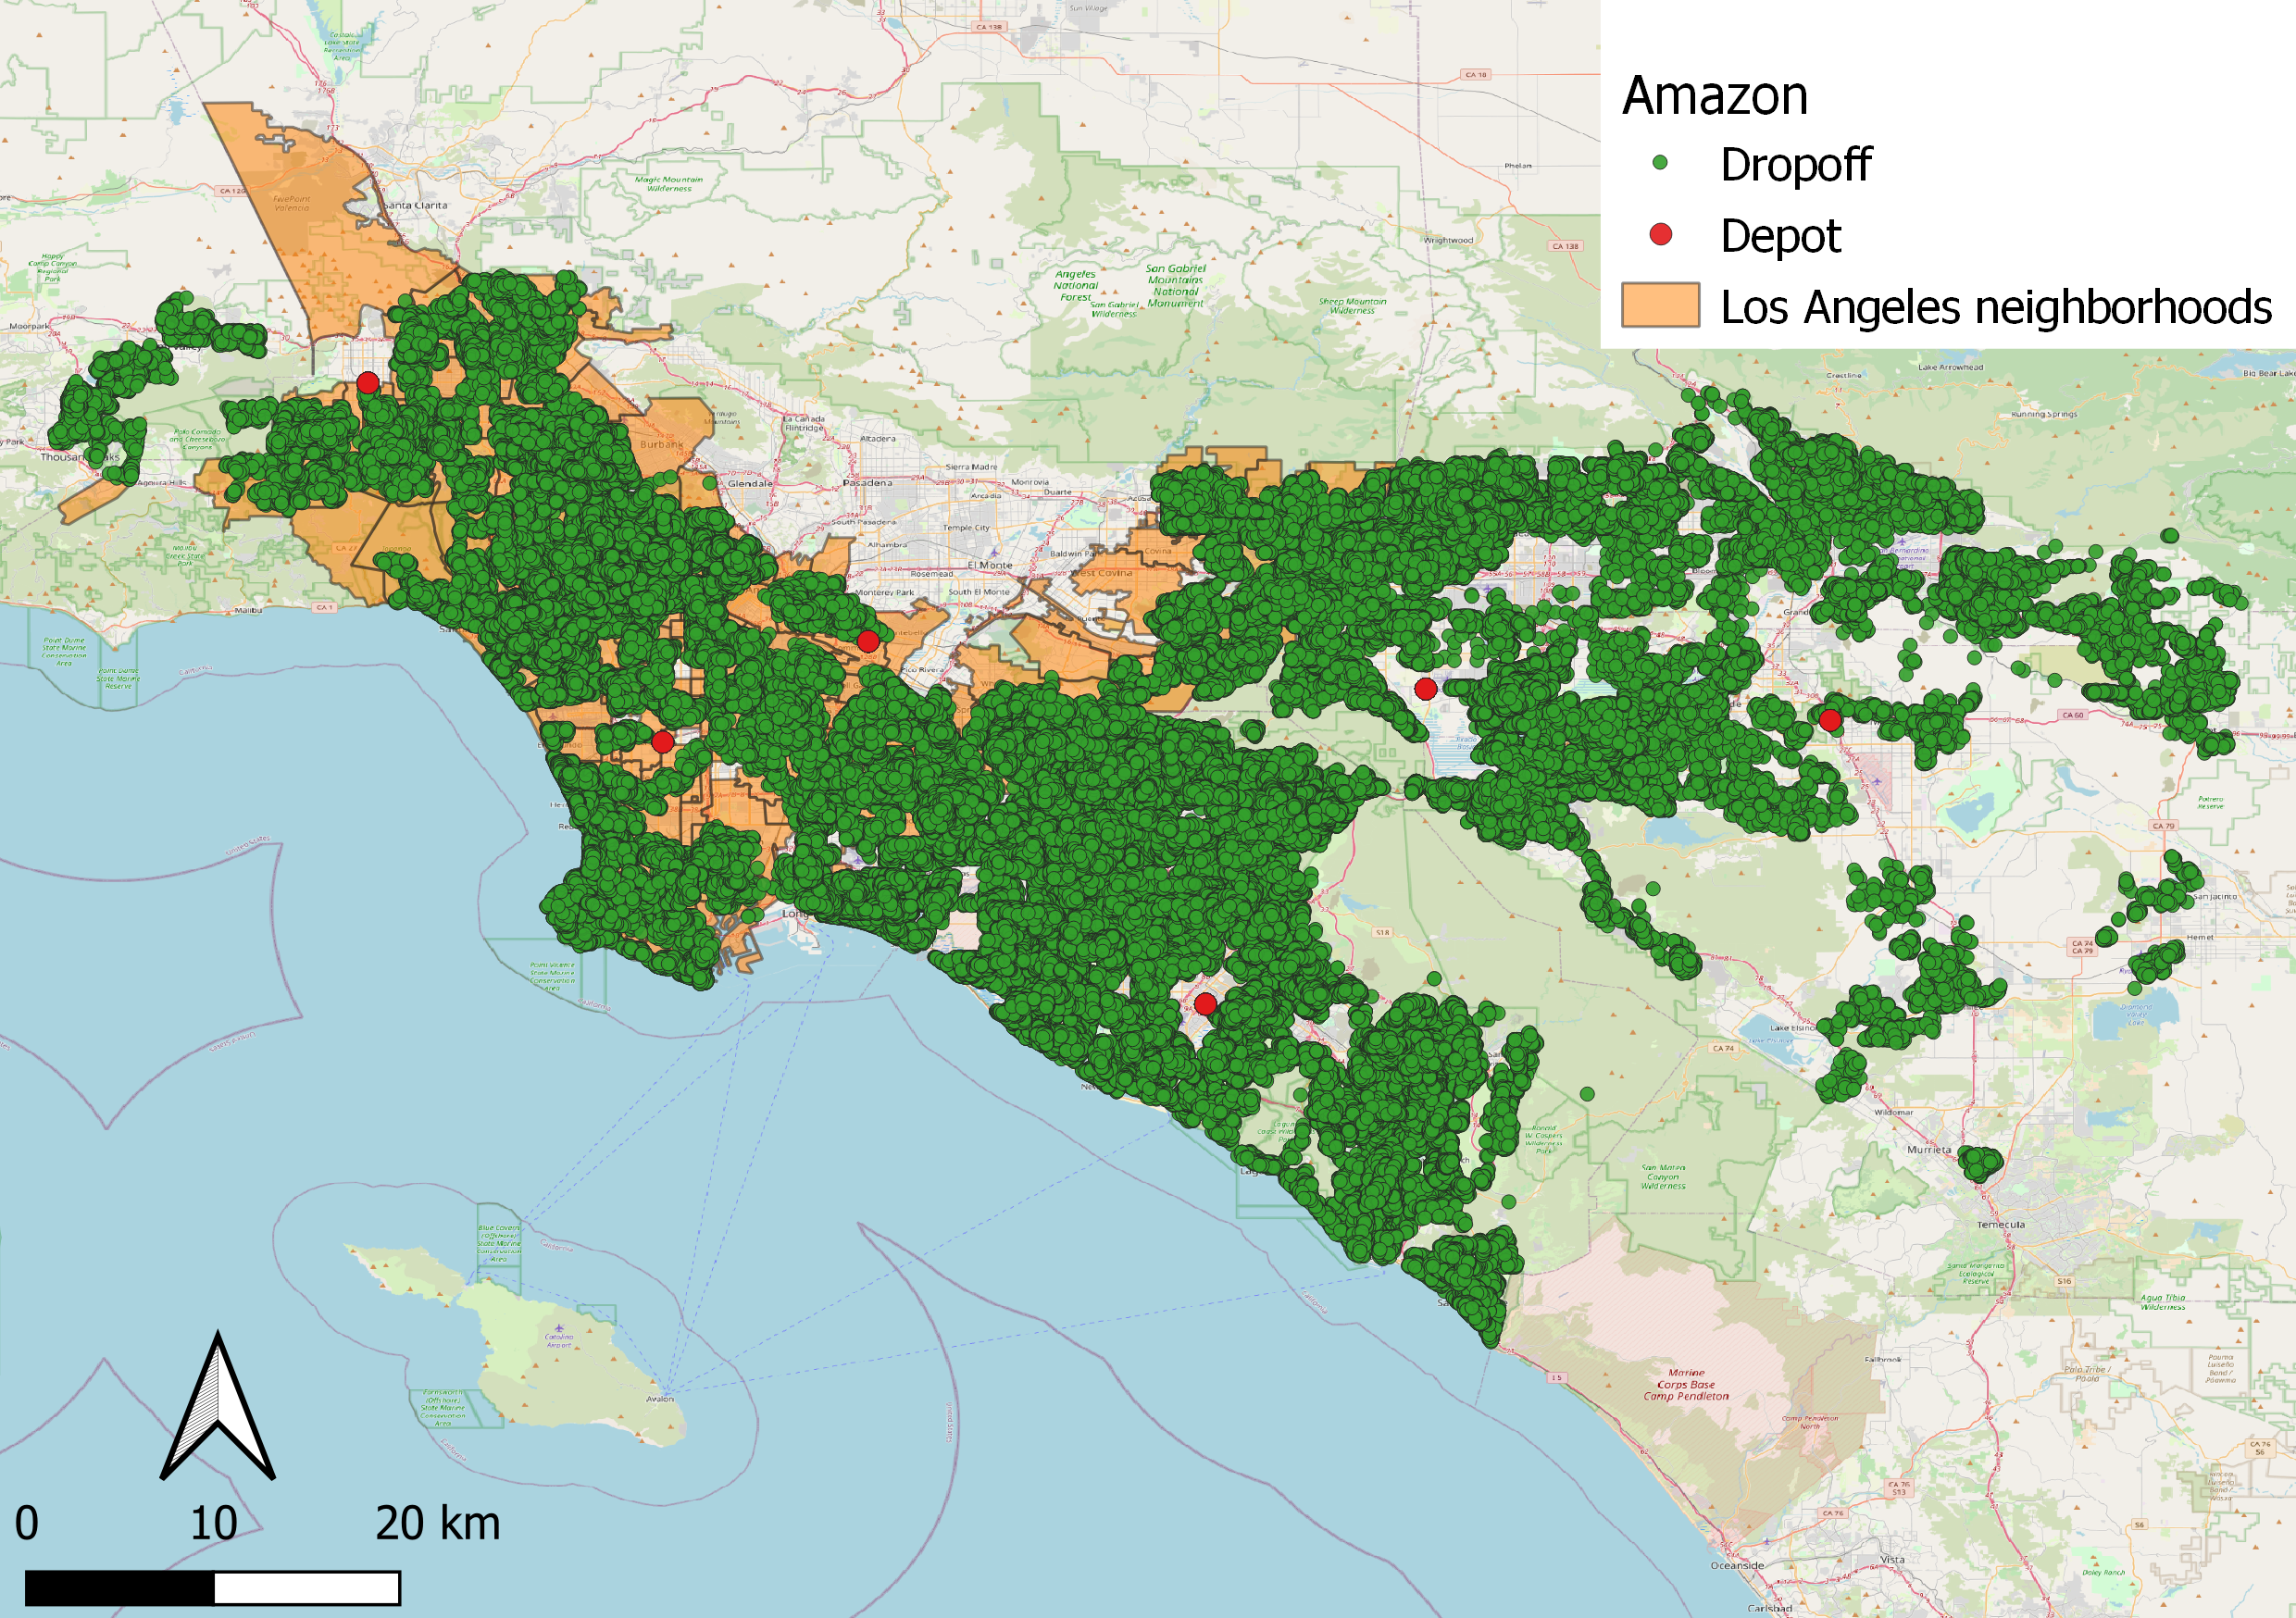
\includegraphics[width=\textwidth]{images/6_amazon/locations/los_angeles_locations.png}
    \end{subfigure}
    %
    \begin{subfigure}{.32\textwidth}
        \caption{Seattle}
        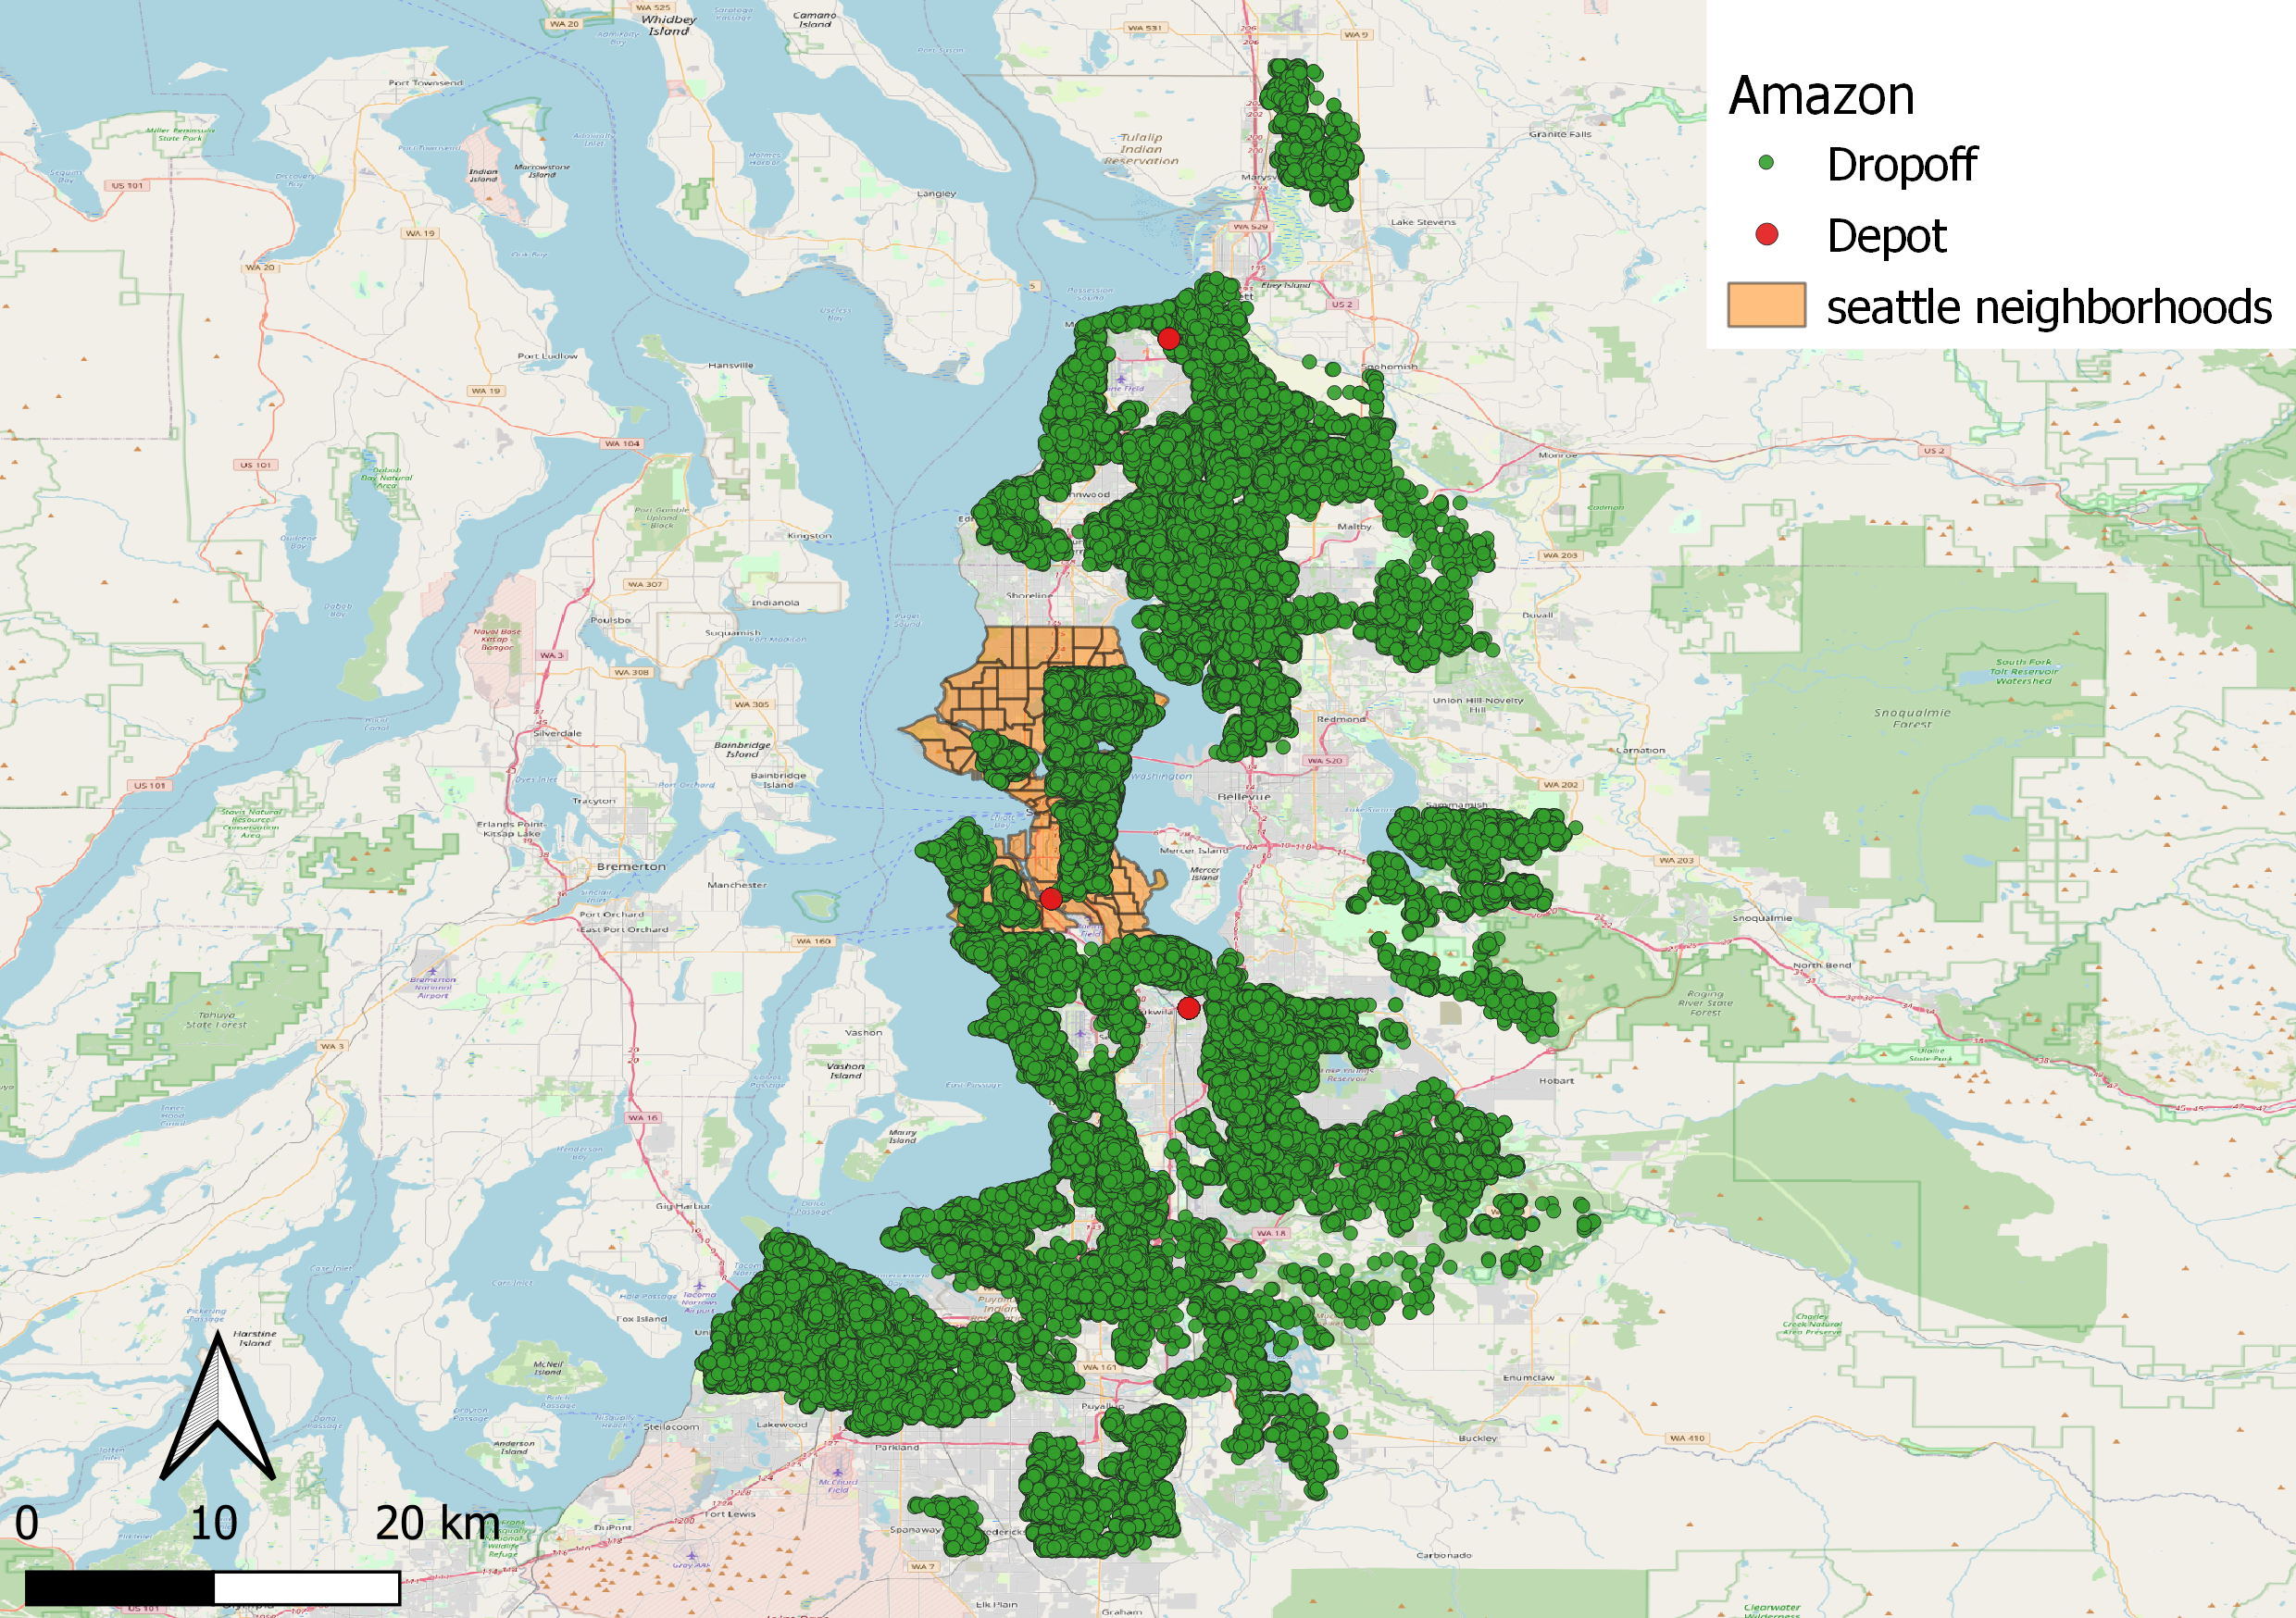
\includegraphics[width=\textwidth]{images/6_amazon/locations/seattle_locations.png}
    \end{subfigure}
    \caption*{\ Fonte: Produzido pelos autores Fernandes \& Alves}
\end{figure}

\singlespacing
\begin{table}[H]
    \centering
    \caption{Percentual de entregas estudadas em relação ao total (Amazon)}
    \label{tab:mantidos_amazon}
    \begin{tabular}{|c|ccc|}
    \hline
    \multicolumn{1}{|c|}{\textbf{Cidade}} & \multicolumn{1}{c|}{\textbf{Entregas Totais}} & \multicolumn{1}{c|}{\textbf{Entregas Estudadas}} & \textbf{\% do total} \\ \hline
    Austin & 31274 & 10000 & 32 \\
    Boston & 140622 & 37283 & 27 \\
    Chicago & 162410 & 26280 & 16 \\
    Los Angeles & 414440 & 144411 & 35 \\
    Seattle & 155771 & 34276 & 22 \\ \hline
    \textbf{Total} & 904517 & 252250 & 28 \\ \hline
    \end{tabular}
    \caption*{\ Fonte: Produzido pelos autores Fernandes \& Alves}
\end{table}
\onehalfspacing

%%%%%%%%%%%%%%%%%%%%%%%%%%%%%%%%%%%
\section{Descrição temporal}

A base de dados disponibilizada contempla um total de trinta e oito dias de operação de entregas da \textit{Amazon}, contudo, este valor varia de acordo com a cidade analisada, conforme pode ser observado na tabela \ref{tab:timesAmazon}.
%
\begin{table}[H]
    \centering
    \caption{Intervalo de tempo observado em de cada cidade (\textit{Amazon})} \label{tab:timesAmazon}
    \begin{tabular}{|cccc|}
        \hline
        \textbf{Cidade} & \textbf{Início} & \textbf{Fim} & \textbf{Dias} \\ \hline
        Austin          & 20-Jul-18       & 17-Aug-18    & 28            \\
        Boston          & 20-Jul-18       & 17-Aug-18    & 28            \\
        Chicago         & 19-Jul-18       & 17-Aug-18    & 29            \\
        Los Angeles     & 19-Jul-18       & 26-Aug-18    & 38            \\
        Seattle         & 19-Jul-18       & 26-Aug-18    & 38            \\ \hline
        \textbf{Total}  & 19-Jul-18       & 26-Aug-18    & 38            \\ \hline
    \end{tabular}
    \caption*{Fonte: Produzido pelos autores Fernandes \& Alves}
\end{table}
%
A Figura \ref{fig:amazon_times} apresenta a distribuição do número de entregas realizadas em cada uma das cidades ao longo do tempo.
Destaca-se que a cidade de Los Angeles apresenta a maior taxa de entregas diárias dentre as cidades analisadas, atingindo mais de $20000$ (vinte mil) entregas em um dos dias observados. 
Contudo, inexplicavelmente, há uma queda no número de entregas a partir do dia 18 de agosto de 2018.
Por outro lado, Austin tem a menor taxa de entregas diária, apesar de apresentar valores mais regulares ao longo do tempo.
%
\begin{figure}[H]
    \centering
    \caption{Distribuição temporal de entregas nas cinco operações estudadas (Amazon)}
    \label{fig:amazon_times}
    \begin{subfigure}{.45\textwidth}
        % \caption{Austin}
        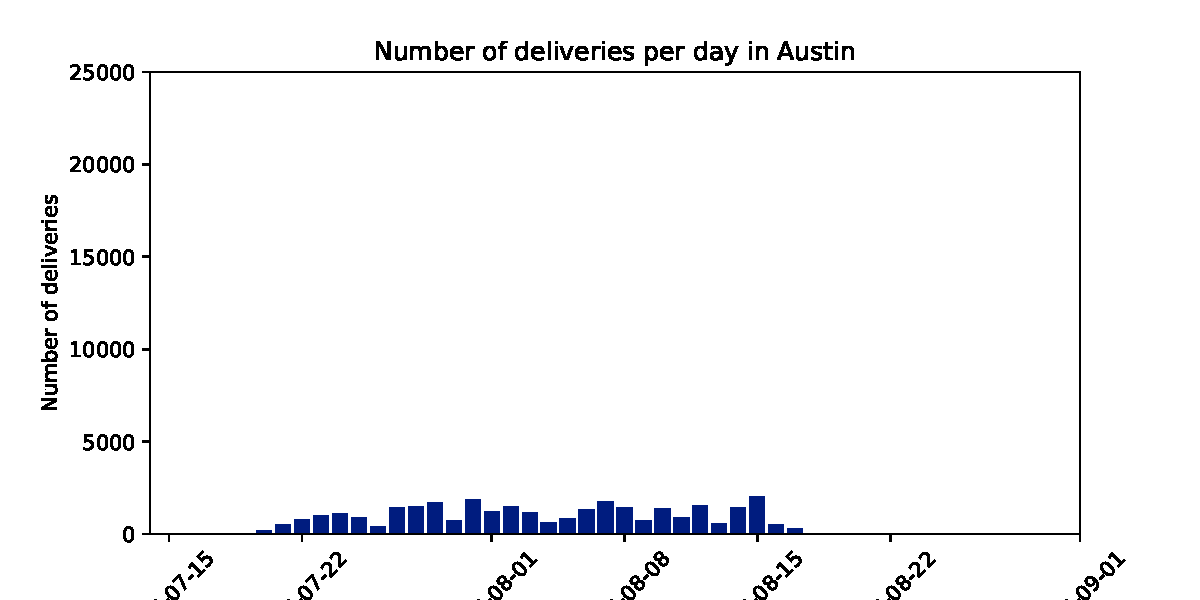
\includegraphics[width=\textwidth]{images/6_amazon/times/austin_deliveries_times.pdf}
    \end{subfigure}
    %
    \begin{subfigure}{.45\textwidth}
        % \caption{Boston}
        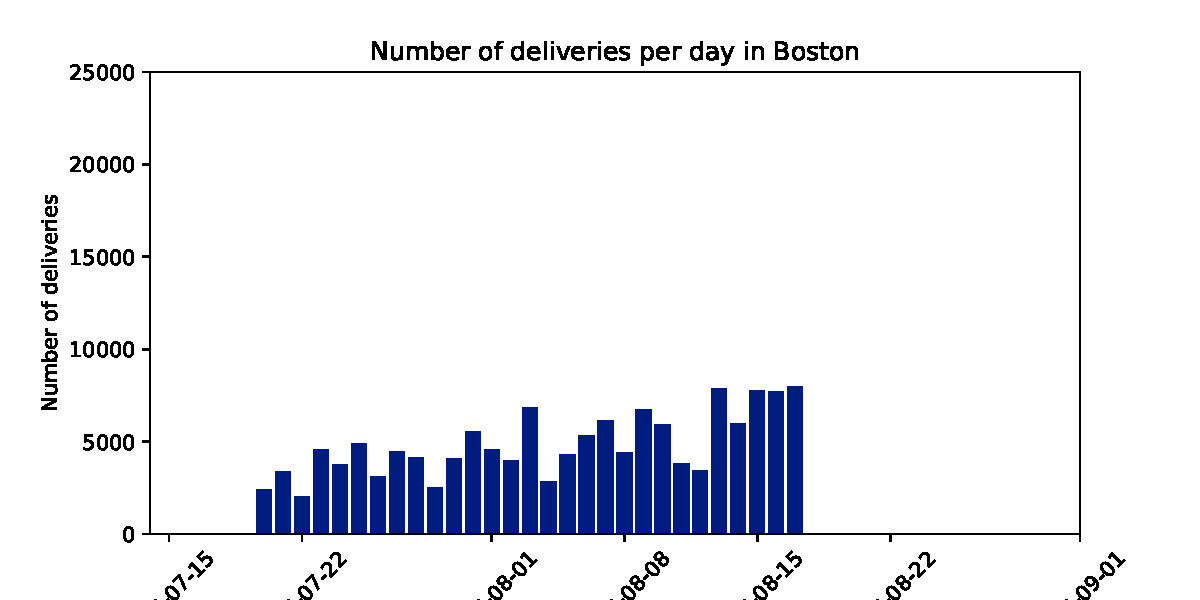
\includegraphics[width=\textwidth]{images/6_amazon/times/boston_deliveries_times.pdf}
    \end{subfigure}
    %
    \begin{subfigure}{.45\textwidth}
        % \caption{Chicago}
        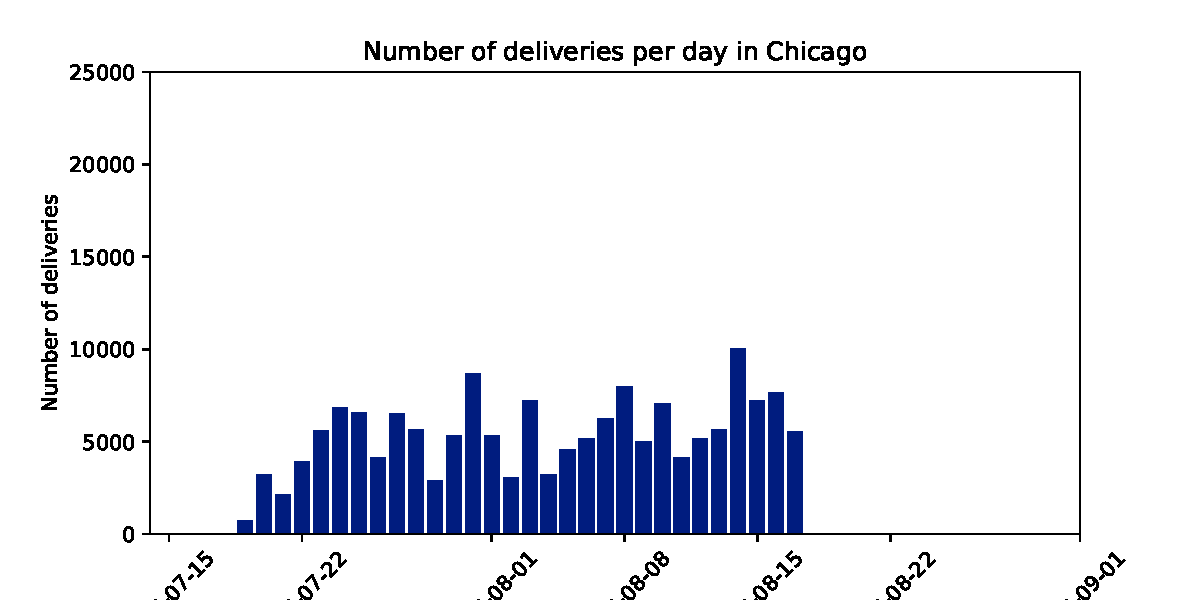
\includegraphics[width=\textwidth]{images/6_amazon/times/chicago_deliveries_times.pdf}
    \end{subfigure}
    %
    \begin{subfigure}{.45\textwidth}
        % \caption{Los Angeles}
        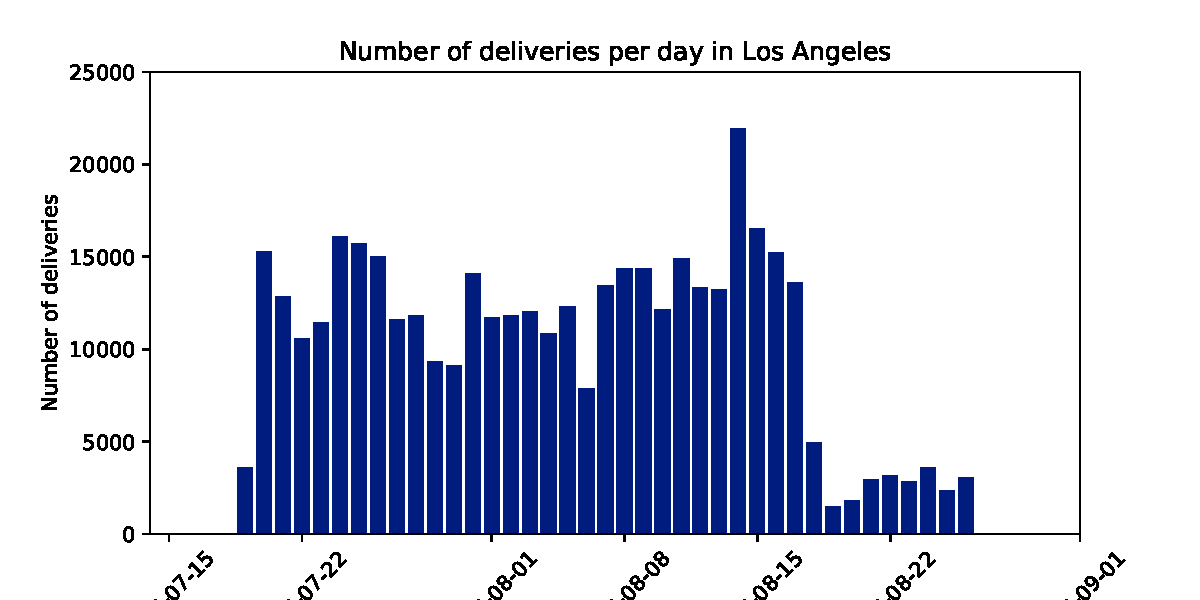
\includegraphics[width=\textwidth]{images/6_amazon/times/la_deliveries_times.pdf}
    \end{subfigure}
    %
    \begin{subfigure}{.45\textwidth}
        % \caption{Seattle}
        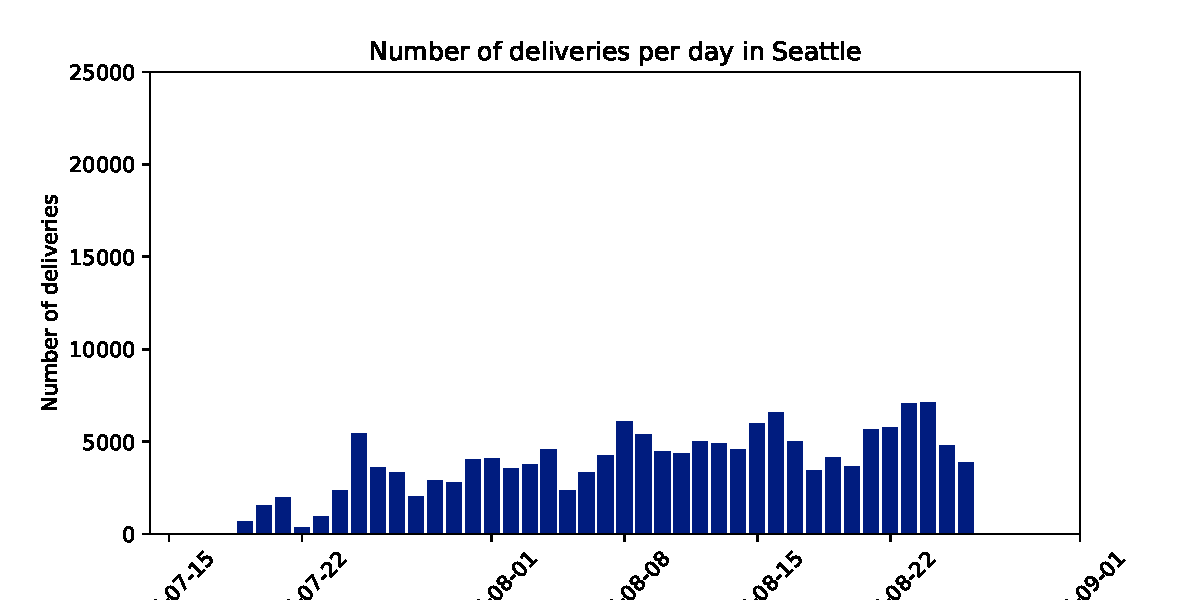
\includegraphics[width=\textwidth]{images/6_amazon/times/seattle_deliveries_times.pdf}
    \end{subfigure}
    \caption*{Fonte: Produzido pelos autores Fernandes \& Alves}
\end{figure}


%%%%%%%%%%%%%%%%%%%%%%%%%%%%%%%%%%%%%%%%%%%%%%%%%%%%%%%%%%
\section{Quantidade de Entregas, Repasses e Devoluções}

Conforme já mencionado na Seção \ref{sec:loc_geografica_amazon}, um total de 6112 rotas estão disponíveis na base de dados estudada.
Cada rota é composta por diferentes PDEs e cada PDE recebe uma certa quantidade de pacotes.
O percentual de repasses e devoluções foi calculado em relação ao número de pacotes, em vez de se calcular em relação ao número de entregas, como foi feito no caso da empresa de bebidas. 
Este método de cálculo é justificado pelo fato de as entregas da \textit{Amazon} permitirem que parte dos pacotes de uma entrega seja devolvida e outra parte entregue.
Dessa forma, estes percentuais tendem a ser relativamente menores do que os apresentados no estudo de caso anterior. 

A contagem do número de rotas em cada uma das cinco cidades pode ser vista na Tabela \ref{tab:resumo_dev_rep_Amazon}, assim como o percentual de repasse e devolução apresentado por cada uma das cidades.
A partir das informações, pode-se destacar que apenas $0.075\%$ dos pacotes foram repassados, sendo que a cidade de Los Angeles possui a taxa de repasses mais elevada dentre as cinco cidades e apenas $0.002\%$ dos pacotes foram devolvidos.

\singlespacing
\begin{table}[H]
    \caption{Entregas, devoluções e repasses por cidade (\textit{Amazon})}
    \label{tab:resumo_dev_rep_Amazon}
    \centering
    \begin{tabular}{|ccc|}
        \hline
        \textbf{Cidade} &
          \textbf{Repasse (\%)} &
          \textbf{Devolução (\%)} \\ \hline
            Austin         & 0.593 & 0.004 \\
            Boston         & 0.553 & 0.000 \\
            Chicago        & 0.545 & 0.003 \\
            Los Angeles    & 0.933 & 0.003 \\
            Seattle        & 0.679 & 0.002 \\ \hline
            \textbf{Total} & \textbf{0.749} & \textbf{0.002} \\ \hline
    \end{tabular}
    \caption*{\ Fonte: Produzido pelos autores Fernandes \& Alves}
\end{table}
\onehalfspacing

A Figura \ref{fig:heatmapAmazon1} apresenta a distribuição espacial de pacotes entregues e pacotes repassados na cidade de Los Angeles. Cita-se que a partir da presente seção, as análises apresentadas serão realizadas a partir dos resultados obtidos no município de Los Angeles. Isso se dá pela maior representatividade que a cidade tem no operação da empresa, além de apresentar maiores índices de repasses. As análises das outras cidades podem ser encontradas na biblioteca pública de códigos da pesquisa, apresentada na bibliografia.
É possível notar uma concentração (ou foco) de repasses na região central da cidade, assim como uma concentração de pacotes entregues também na região central.
Contudo a região de concentração de entregas não é exatamente igual à região de concentração de repasses, o que sugere que provavelmente a região de maior incidência de repasses possui alguma característica - por exemplo, organização da malha viária - que a deixa mais propícia a apresentar rotas com repasses.

\begin{figure}[htb]
    \centering
    \caption{Mapa de calor de entregas e repasses na cidade de Los Angeles (\textit{Amazon})} \label{fig:heatmapAmazon1}
    \begin{subfigure}{0.49\textwidth}
        \caption{Pacotes entregues}
        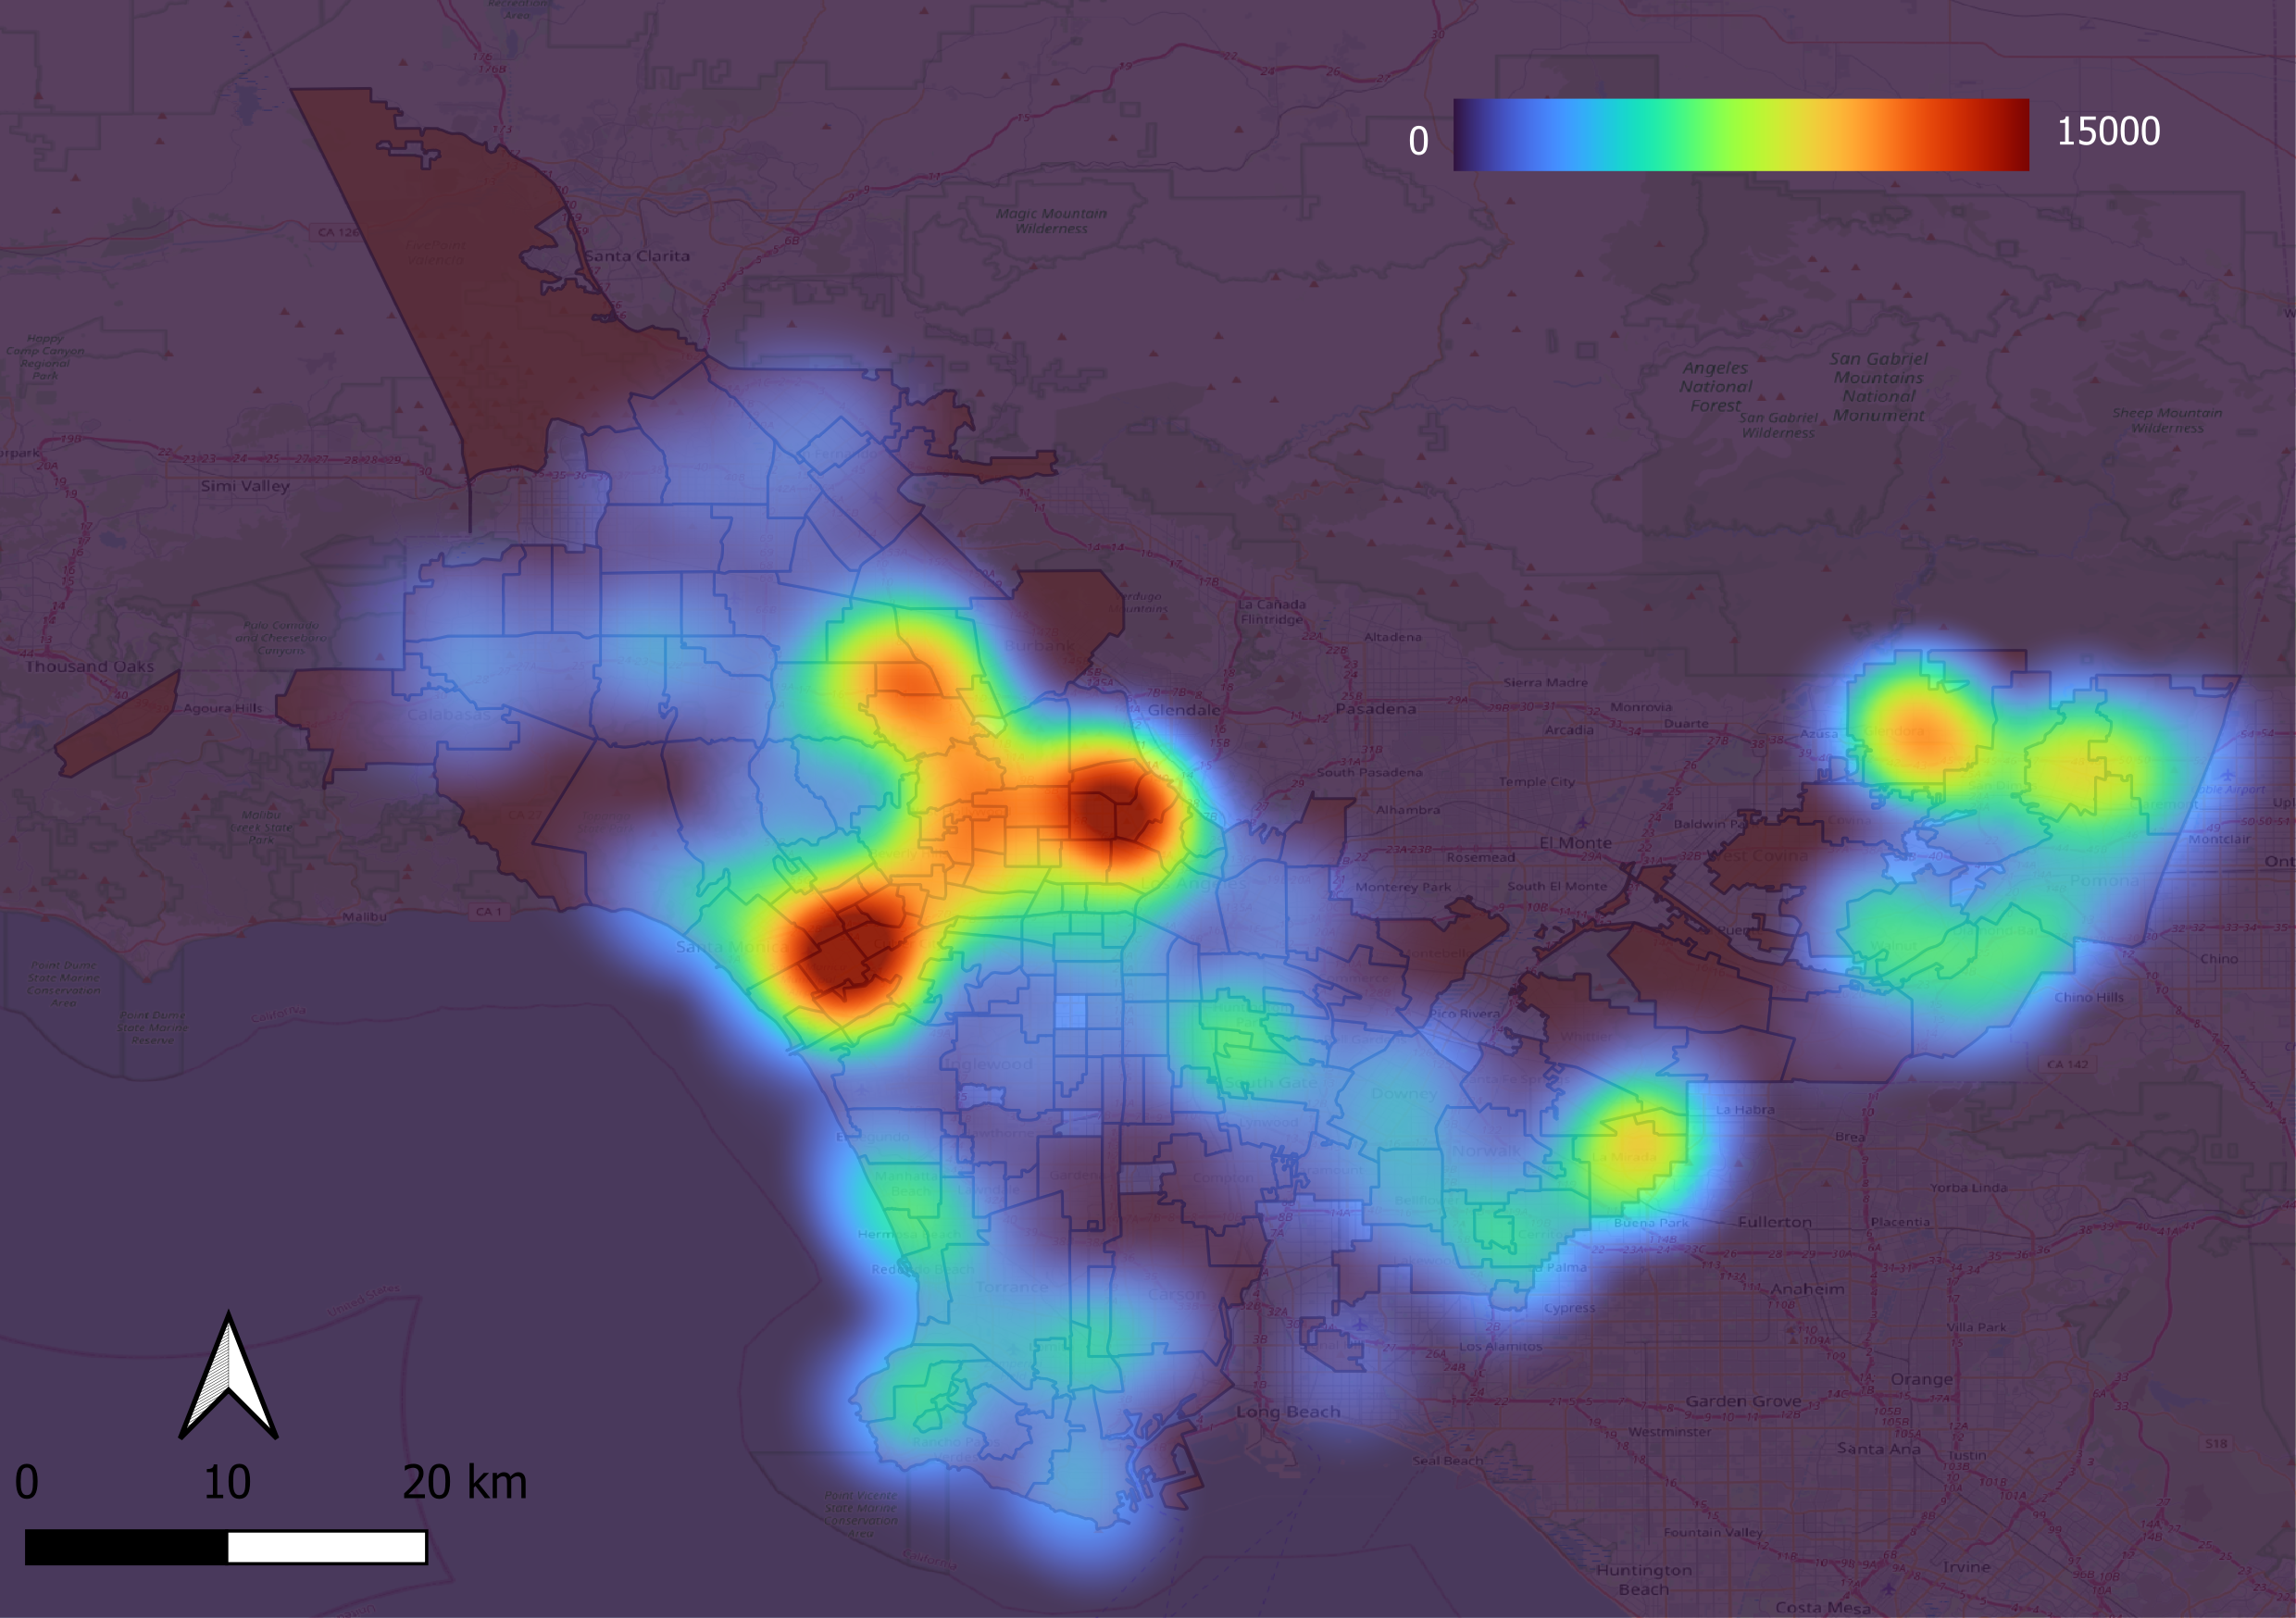
\includegraphics[width=\textwidth]{images/6_amazon/rep_e_dev/los_angeles_entregas.png}
    \end{subfigure}
    \begin{subfigure}{0.49\textwidth}
        \caption{Pacotes repassados}
        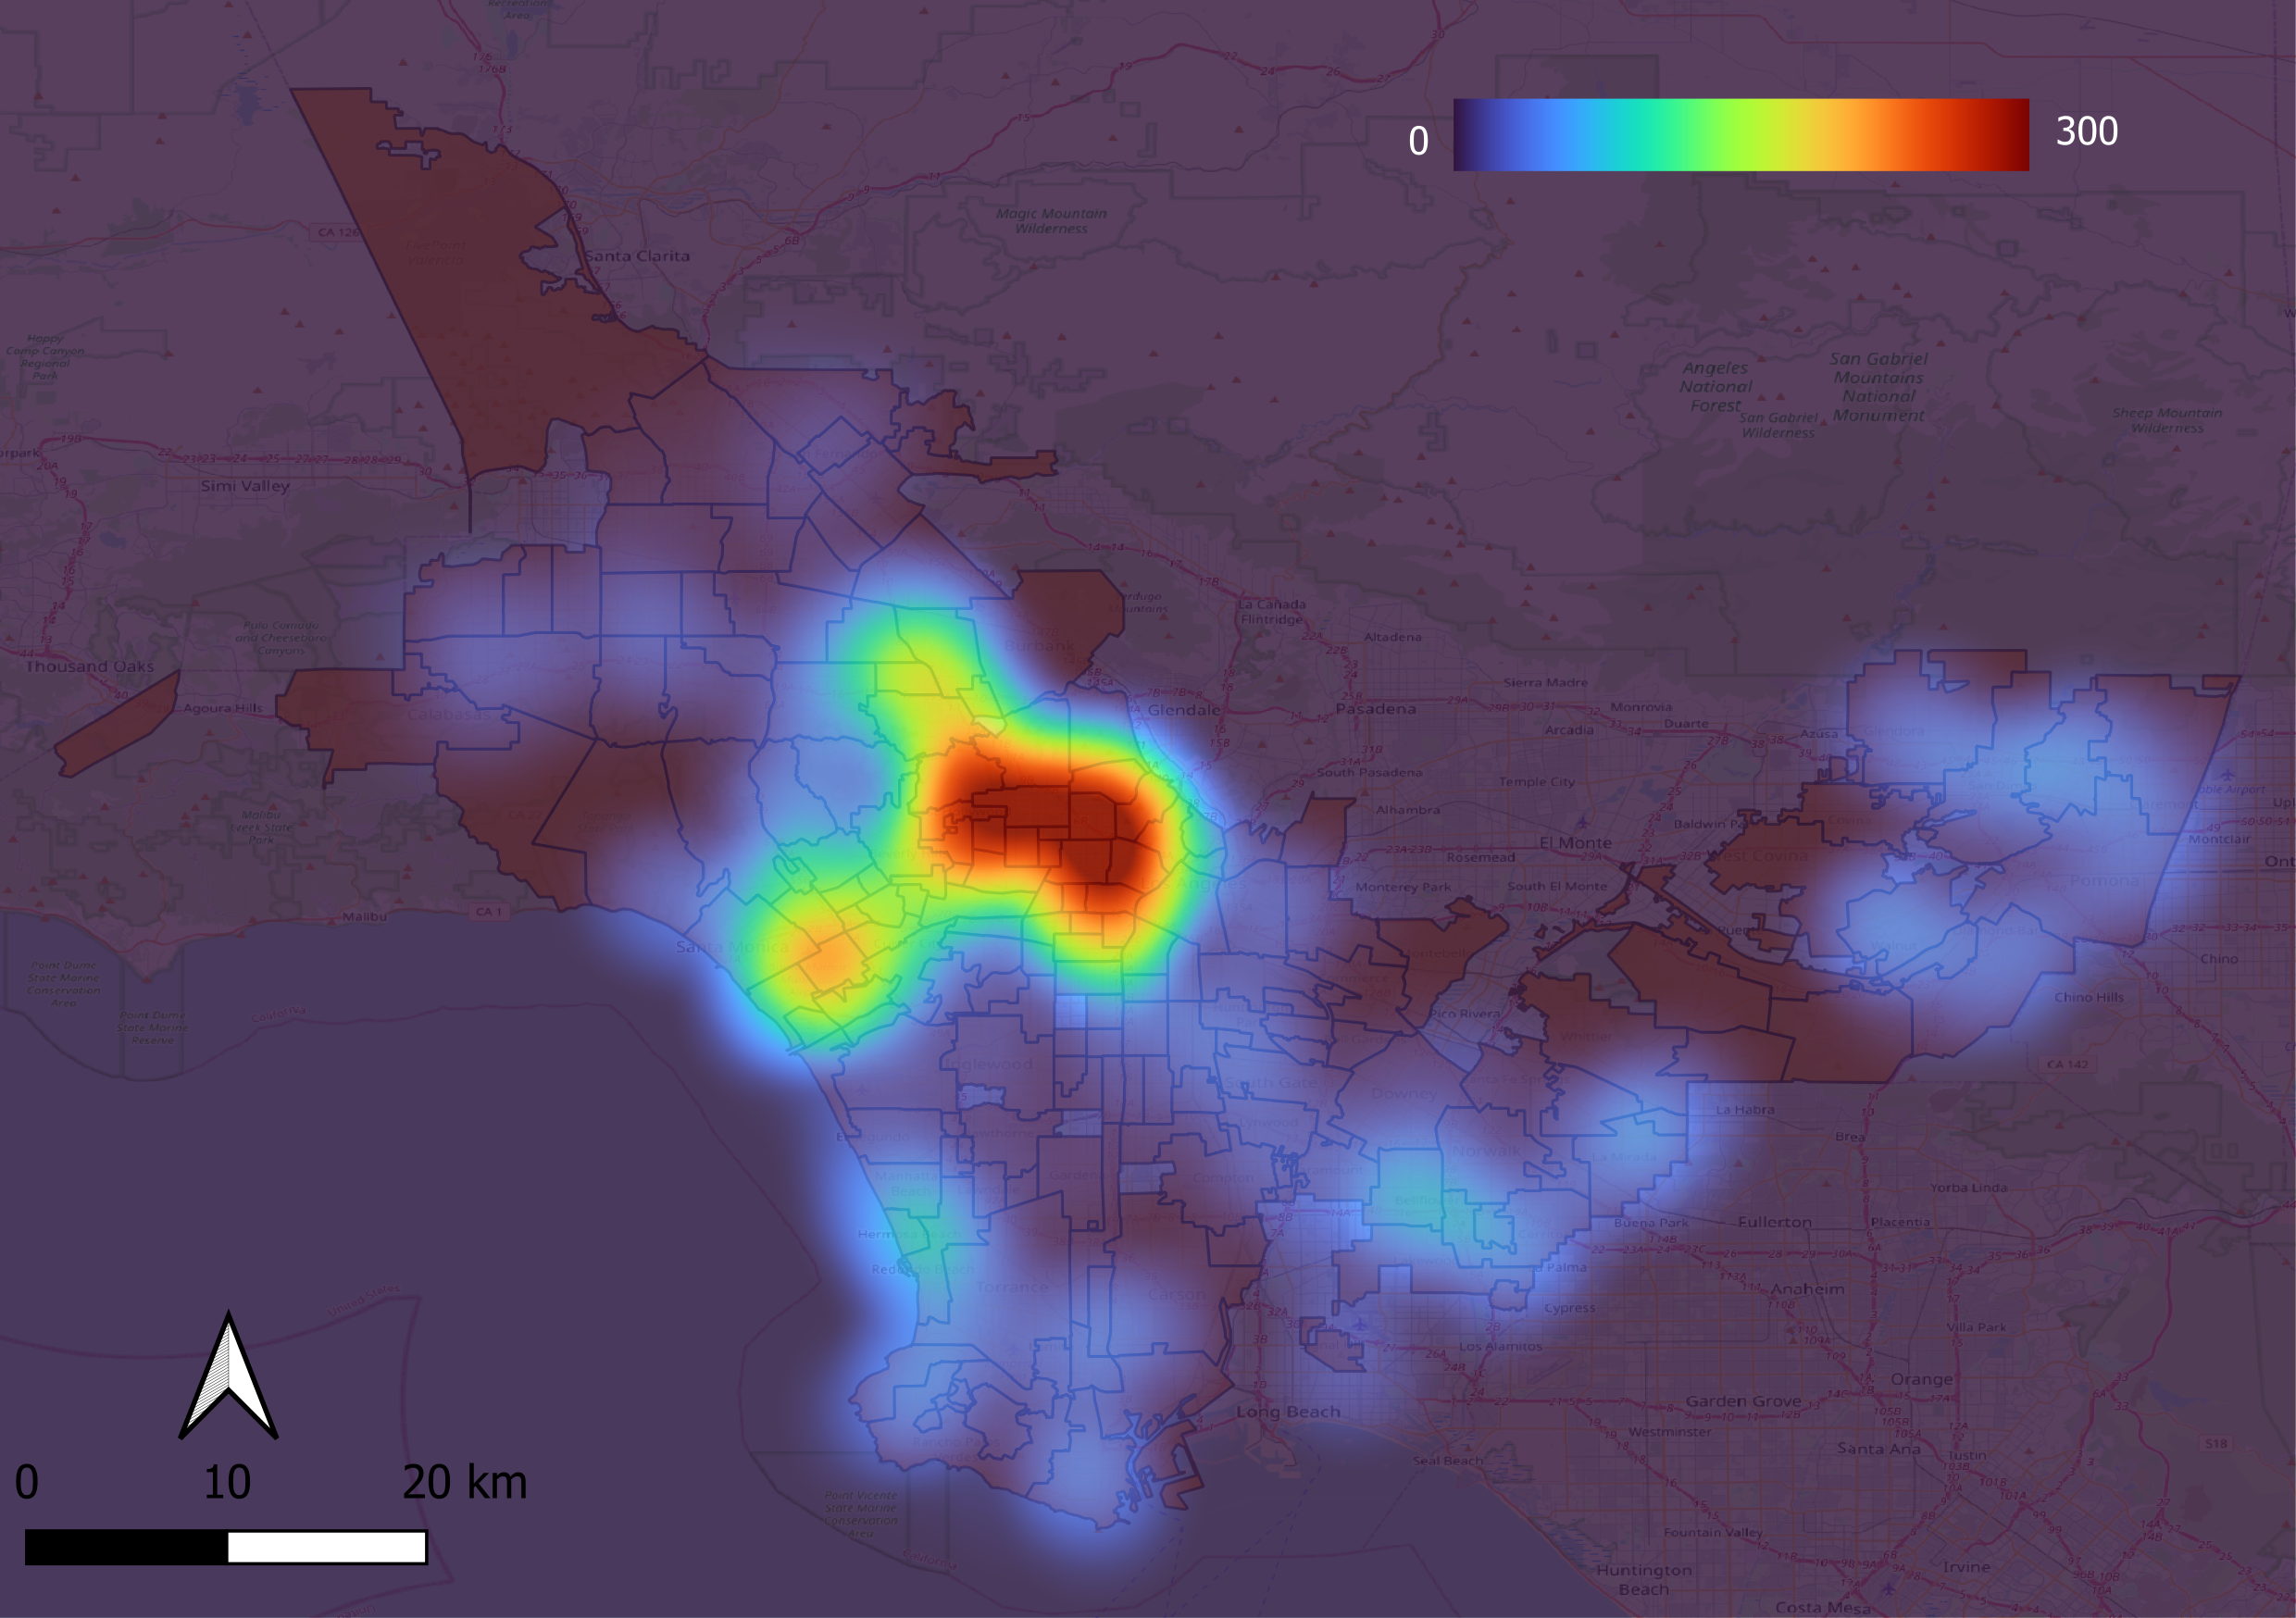
\includegraphics[width=\textwidth]{images/6_amazon/rep_e_dev/los_angeles_failed.png}
    \end{subfigure}
    \caption*{\ Fonte: Produzido pelos autores Fernandes \& Alves}
\end{figure}

A Figura \ref{fig:devolucoes_LA} apresenta a distribuição espacial do número de pacotes devolvidos na cidade de Los Angeles.
Os bairros que apresentam o maior número de devoluções são ``Sherman Oaks'' e ``Hollywood Hills''.
Destaca-se que, mesmo nestes bairros mais problemáticos, apenas dois pacotes foram devolvidos em todas as rotas observadas.

\begin{figure}[H]
    \centering
    \caption{Pacotes devolvidos por bairros da cidade de Los Angeles (\textit{Amazon})}
    \label{fig:devolucoes_LA}
    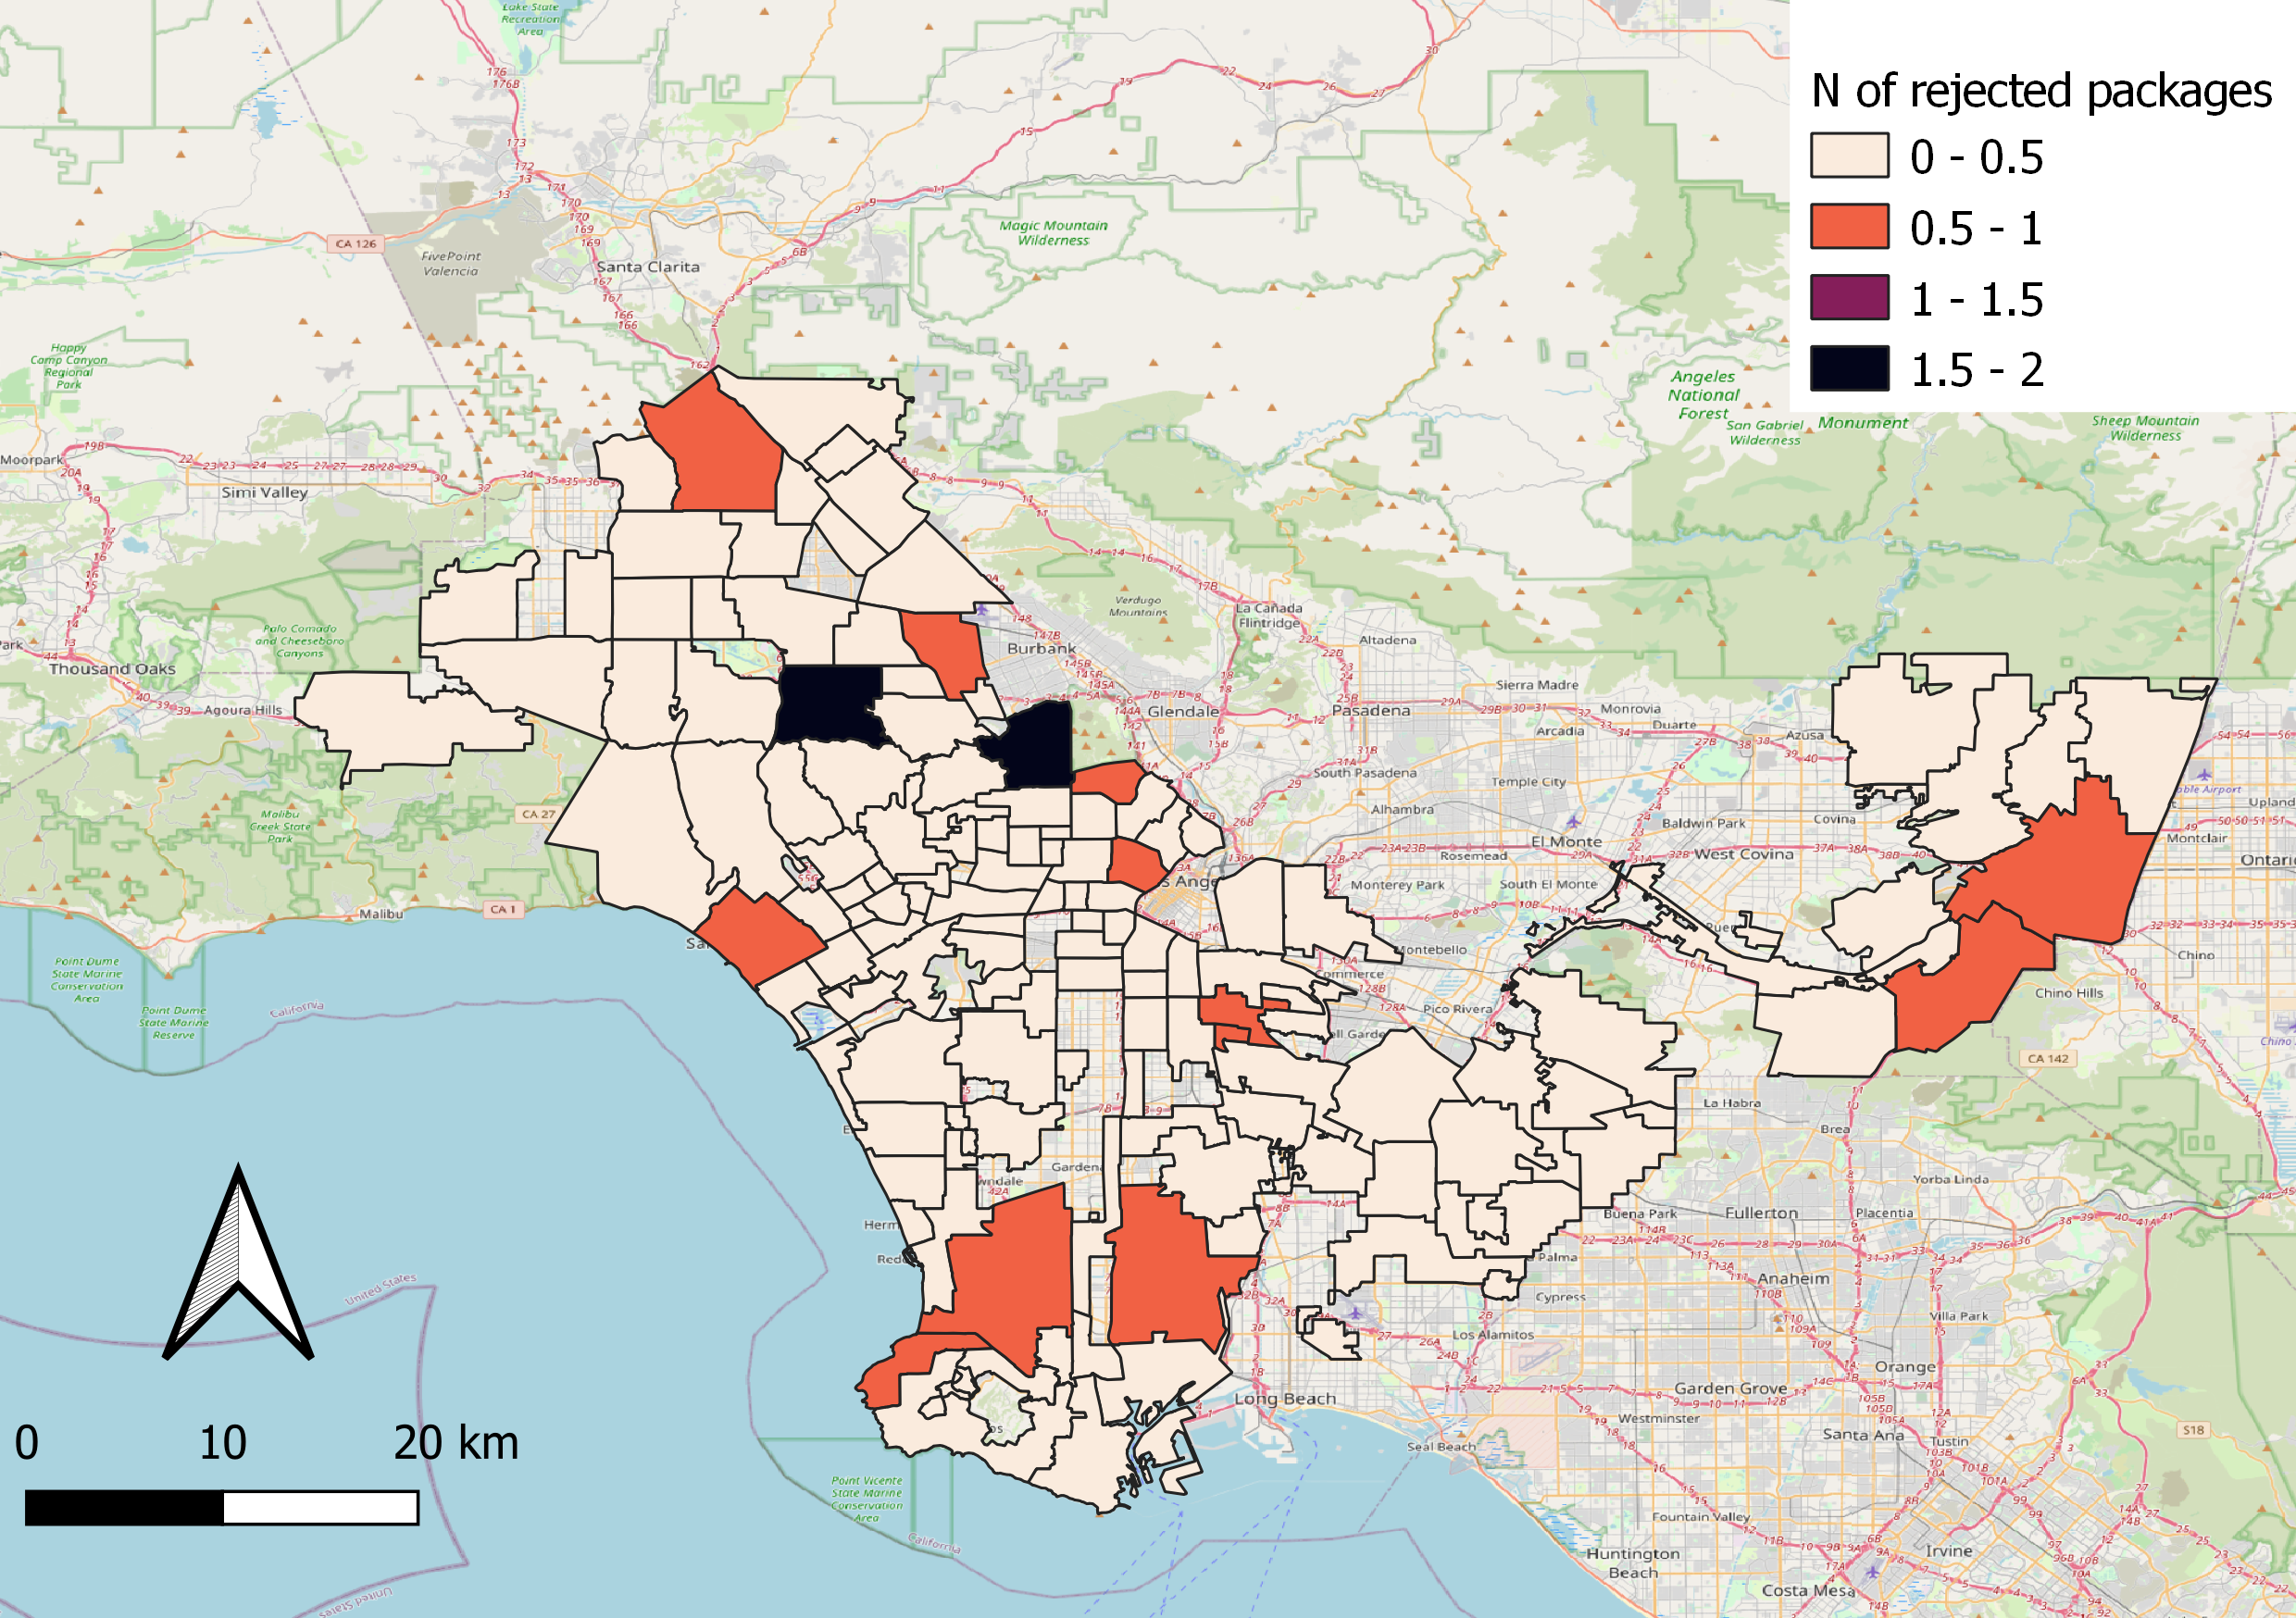
\includegraphics[width=0.7\textwidth]{images/6_amazon/rep_e_dev/los_angeles_rejected.png}
    \caption*{\ Fonte: Produzido pelos autores Fernandes \& Alves}
\end{figure}


%%%%%%%%%%%%%%%%%%%%%%%%%
\section{Geoestatísticas} \label{sec:Amazon_AnalisesPreliminares}

Nas Figuras \ref{fig:AMAZON_LISA_REP} e \ref{fig:AMAZON_LISA_DEV} é possível observar os mapas LISA construídos para a cidade de Los Angeles considerando, respectivamente, os valores de repasse e devolução calculados para cada bairro. 
Ademais, as Figuras \ref{fig:AMAZON_SCT_REP} e \ref{fig:AMAZON_SCT_DEV} indicam numericamente a correlação espacial. 

\begin{figure}[H]
    \centering
     \caption{Correlação espacial do percentual de repasses por bairro (\textit{Amazon})}
     \begin{subfigure}{.45\textwidth}
         \centering
         % include first image 
         \caption{Mapa LISA.}
         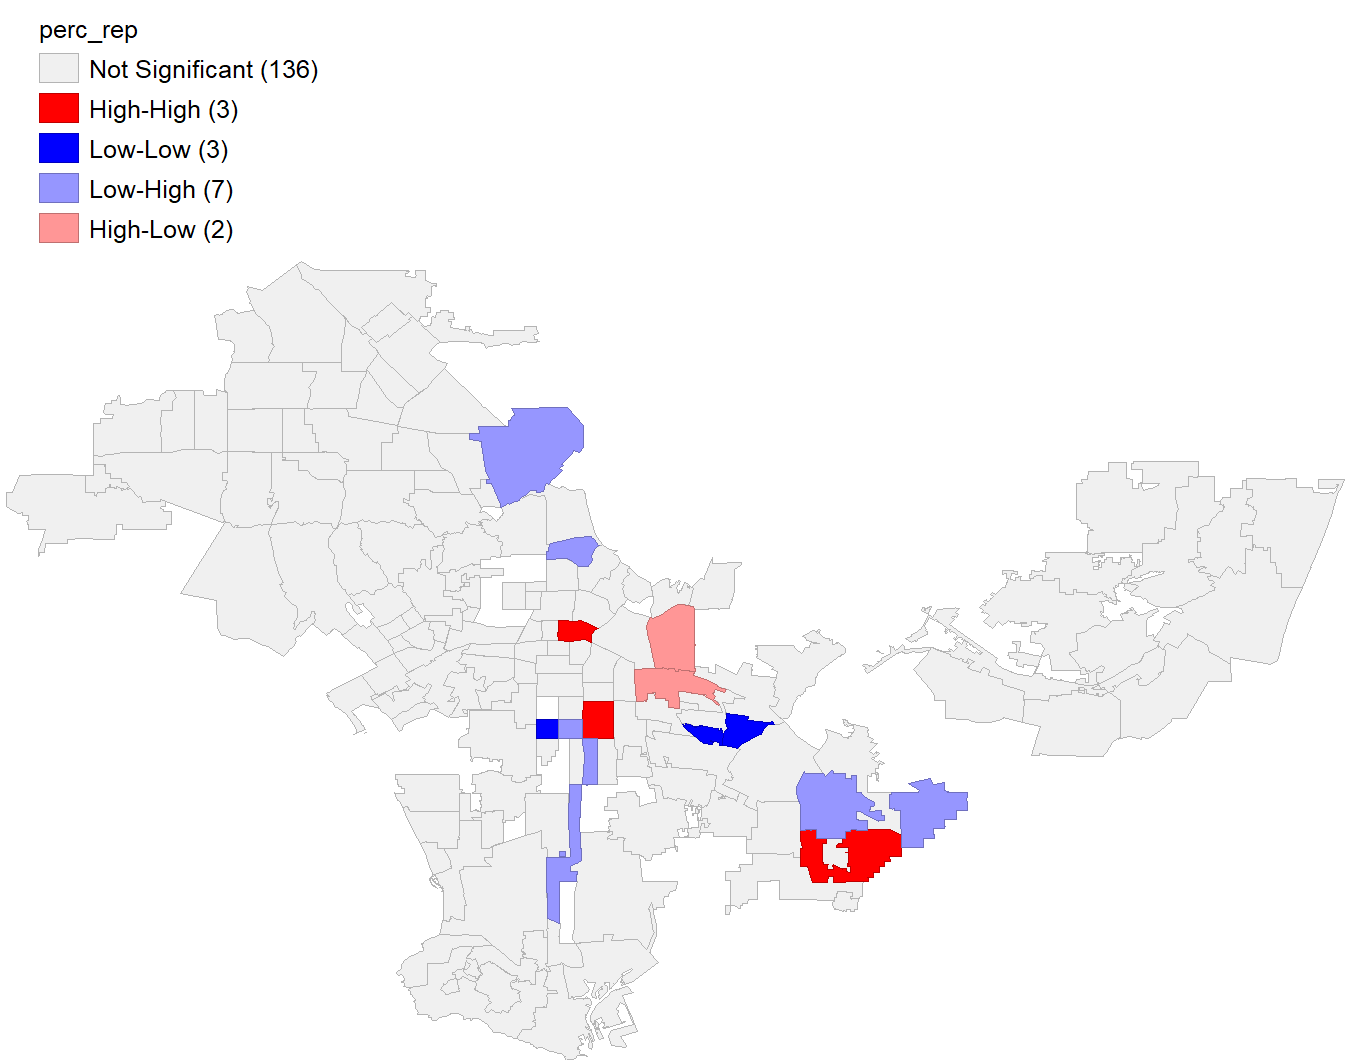
\includegraphics[height=0.75\textwidth]{images/6_amazon/geoda/BairrosLA_REP_lisa.png}
         \label{fig:AMAZON_LISA_REP}
     \end{subfigure}
     \begin{subfigure}{.45\textwidth}
       \centering
       % include second image
       \caption{Gráfico de Dispersão.}
       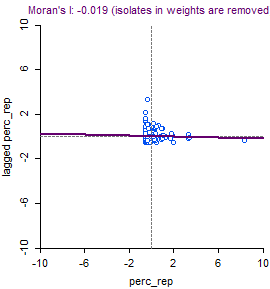
\includegraphics[height=0.75\textwidth]{images/6_amazon/geoda/BairrosLA_REP_scatter.png}
       \label{fig:AMAZON_SCT_REP}
     \end{subfigure}
     \caption*{\ Fonte: Produzido pelos autores Fernandes \& Alves}
 \end{figure} % Repasses

\begin{figure}[H]
    \centering
     \caption{Correlação espacial do percentual de devoluções por bairro (\textit{Amazon})}
     \begin{subfigure}{.45\textwidth}
         \centering
         % include first image 
         \caption{Mapa LISA}
         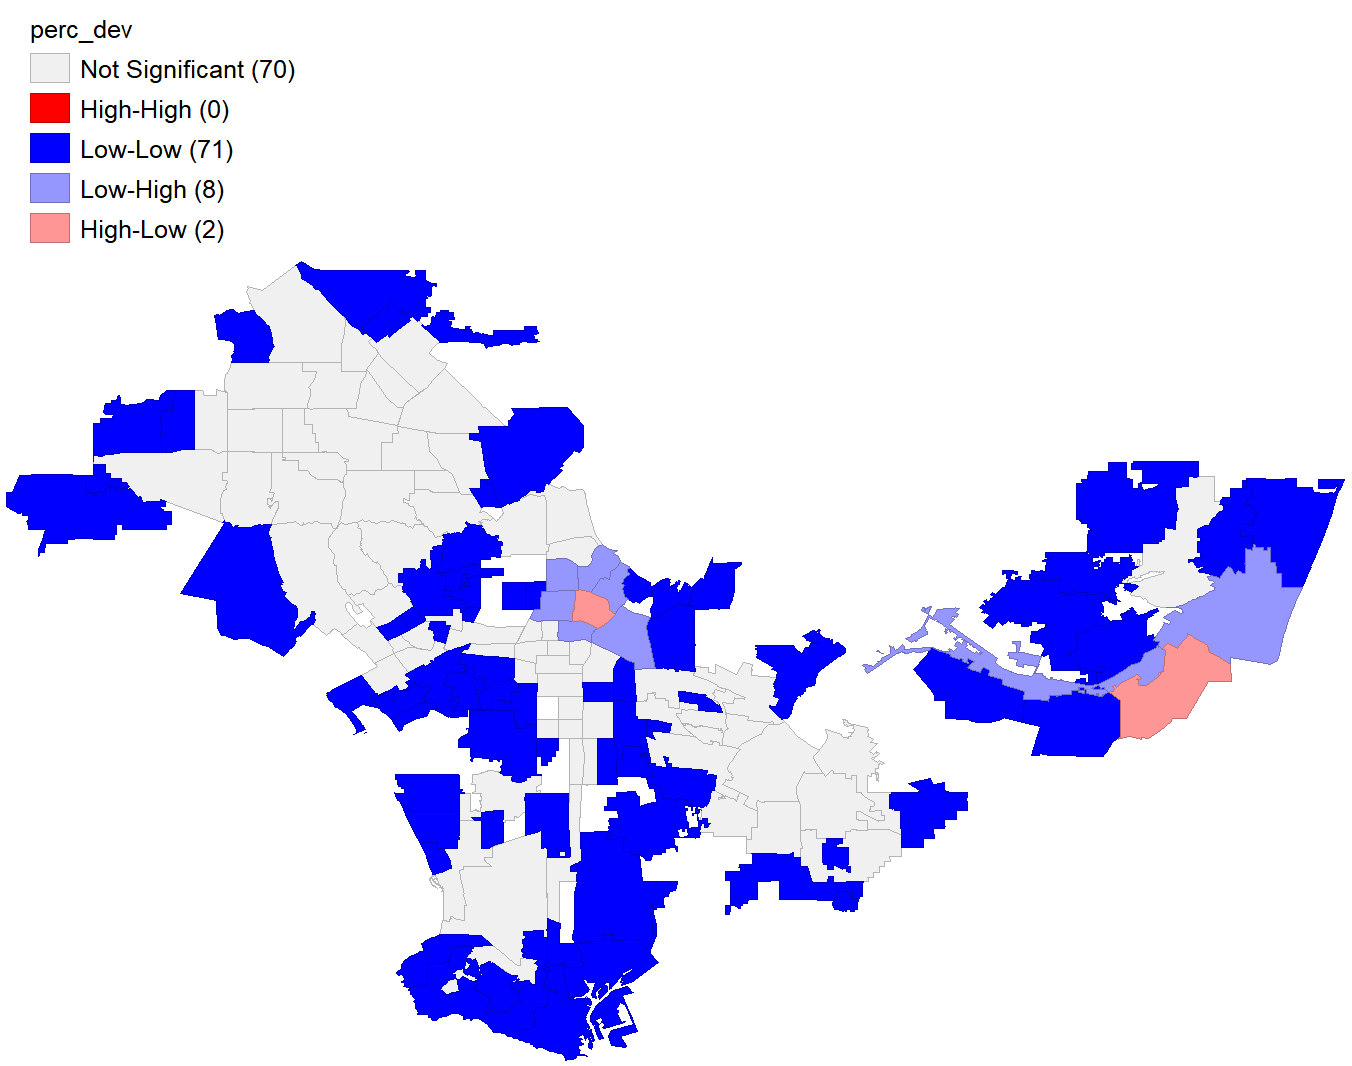
\includegraphics[height=0.75\textwidth]{images/6_amazon/geoda/BairrosLA_DEV_lisa.png}
         \label{fig:AMAZON_LISA_DEV}
     \end{subfigure}
     \begin{subfigure}{.45\textwidth}
       \centering
       % include second image
       \caption{Gráfico de Dispersão.}
       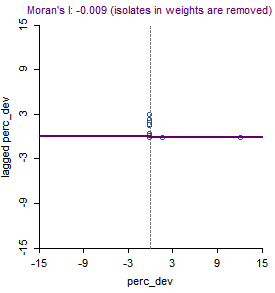
\includegraphics[height=0.75\textwidth]{images/6_amazon/geoda/BairrosLA_DEV_scatter.png}
       \label{fig:AMAZON_SCT_DEV}
     \end{subfigure}
     \caption*{\ Fonte: Produzido pelos autores Fernandes \& Alves}
 \end{figure} % Devoluções

As análises geoestatísticas, de modo geral, apresentaram baixo nível de correlação espacial nos bairros de Los Angeles considerando indicadores de repasse e devolução percentuais. 
A alta ocorrência de bairros classificados como ``LOW-LOW'' no mapa LISA de devoluções percentuais decorre do baixíssimo nível de ocorrência de devoluções na base, o que implica num número alto de bairros com 0\% de devoluções. 

Estes resultados, porém, não eliminam as possibilidades de a geografia dos bairros influenciarem a ocorrência de repasses e devoluções. 
Os resultados representam apenas tendências entre bairros vizinhos. 
Assim, bairros que estejam localizados em regiões distintas da cidade não são comparadores entre si. 
Portanto, nos tópicos seguintes serão analisadas com maiores detalhes as variáveis de repasse de devolução considerando características individuais de cada bairro.

%%%%%%%%%%%%%%%%%%%%%%%%%%%%%%%%%%%%%%%%%%%%%%%%%
\section{Fator de circuito} \label{sec:Amazon_FC}

A fim de se calcular o fator de circuito das rotas analisadas, para cada rota foram somadas as distâncias euclidianas entre os diferentes pontos de entregas, assim como as distâncias veiculares.
A média das distâncias totais das rotas é apresentada na Figura \ref{fig:distanciasRotasLA}, onde estão resumidas por bairros.
É possível identificar que bairros que estão mais distantes dos CDs tendem a conter rotas de maiores distâncias totais, o que é condizente com a estrutura urbana onde se encontram regiões mais densas em áreas centrais da cidade. 
Assim, o veículo realiza maiores deslocamentos para acessar os clientes mais dispersos.

\begin{figure}[H]
    \centering
    \caption{Média de distâncias totais de rotas na cidade de Los Angeles (\textit{Amazon})} \label{fig:distanciasRotasLA}
    \begin{subfigure}{0.45\textwidth}
        \caption{Distância Euclidiana}
        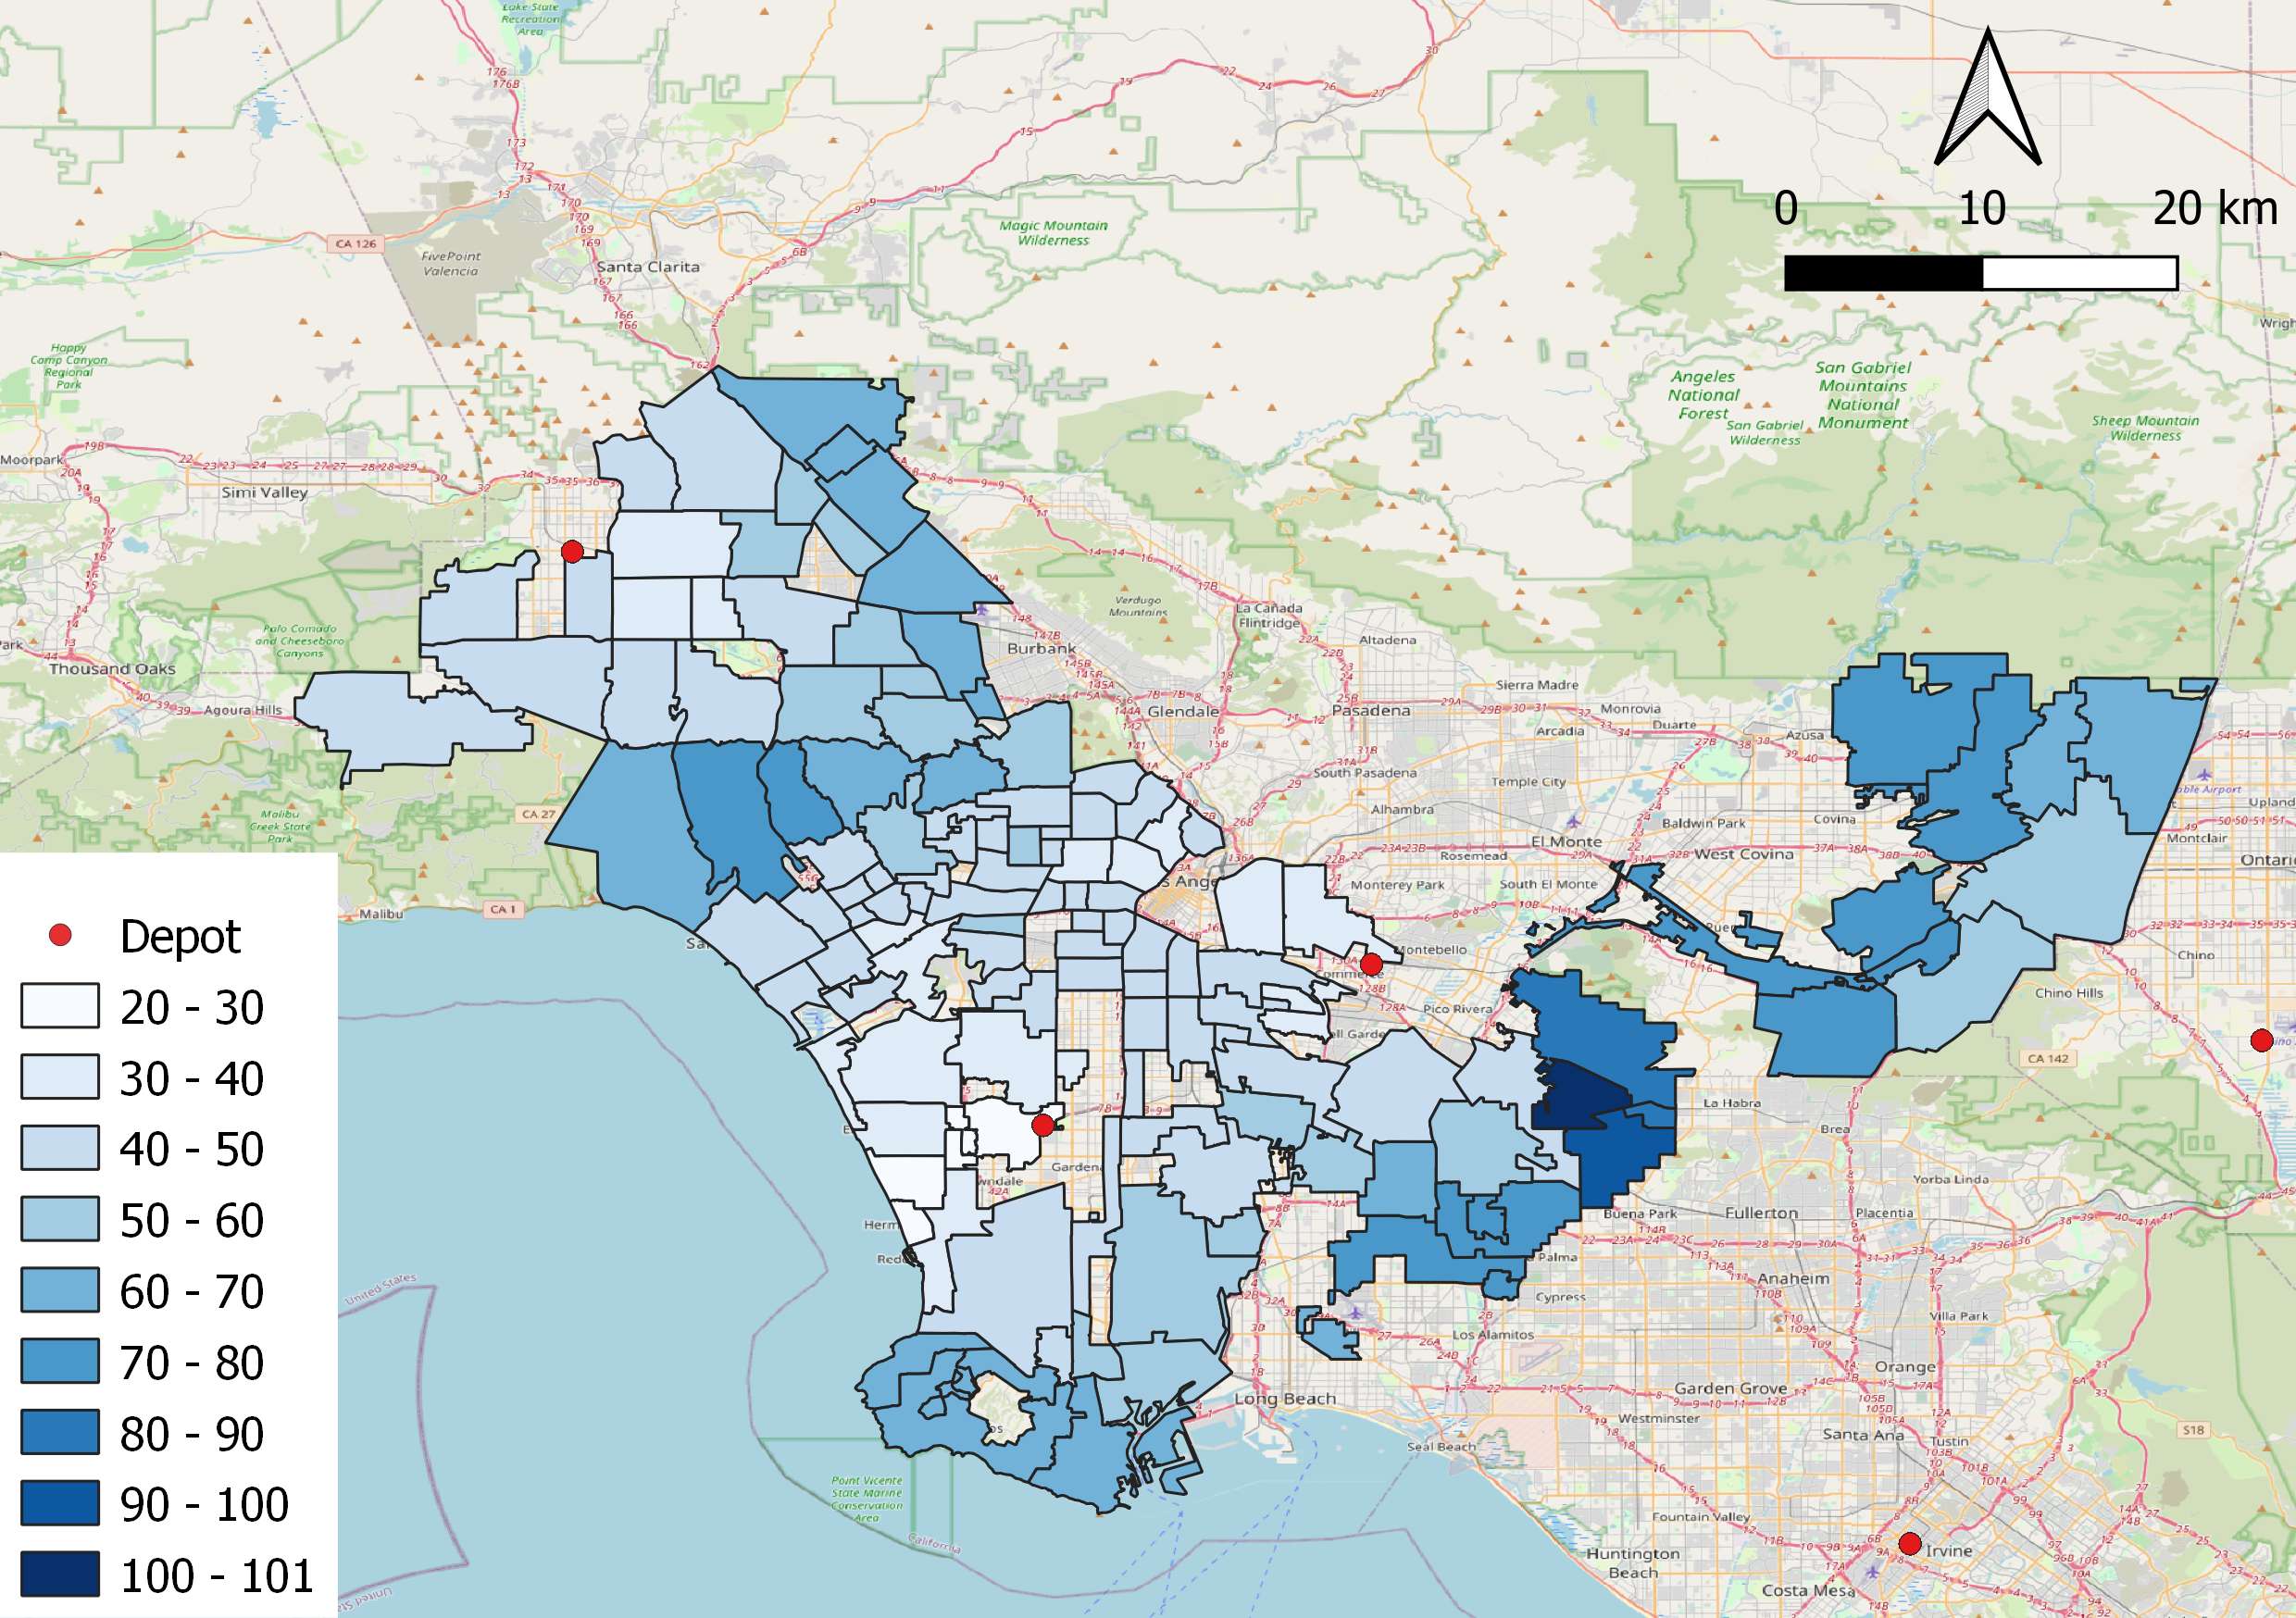
\includegraphics[width=\textwidth]{images/6_amazon/distancias/Avg Sum of Euc. Dist. Route - LA.png}
    \end{subfigure}
    \begin{subfigure}{0.45\textwidth}
        \caption{Distância veicular}
        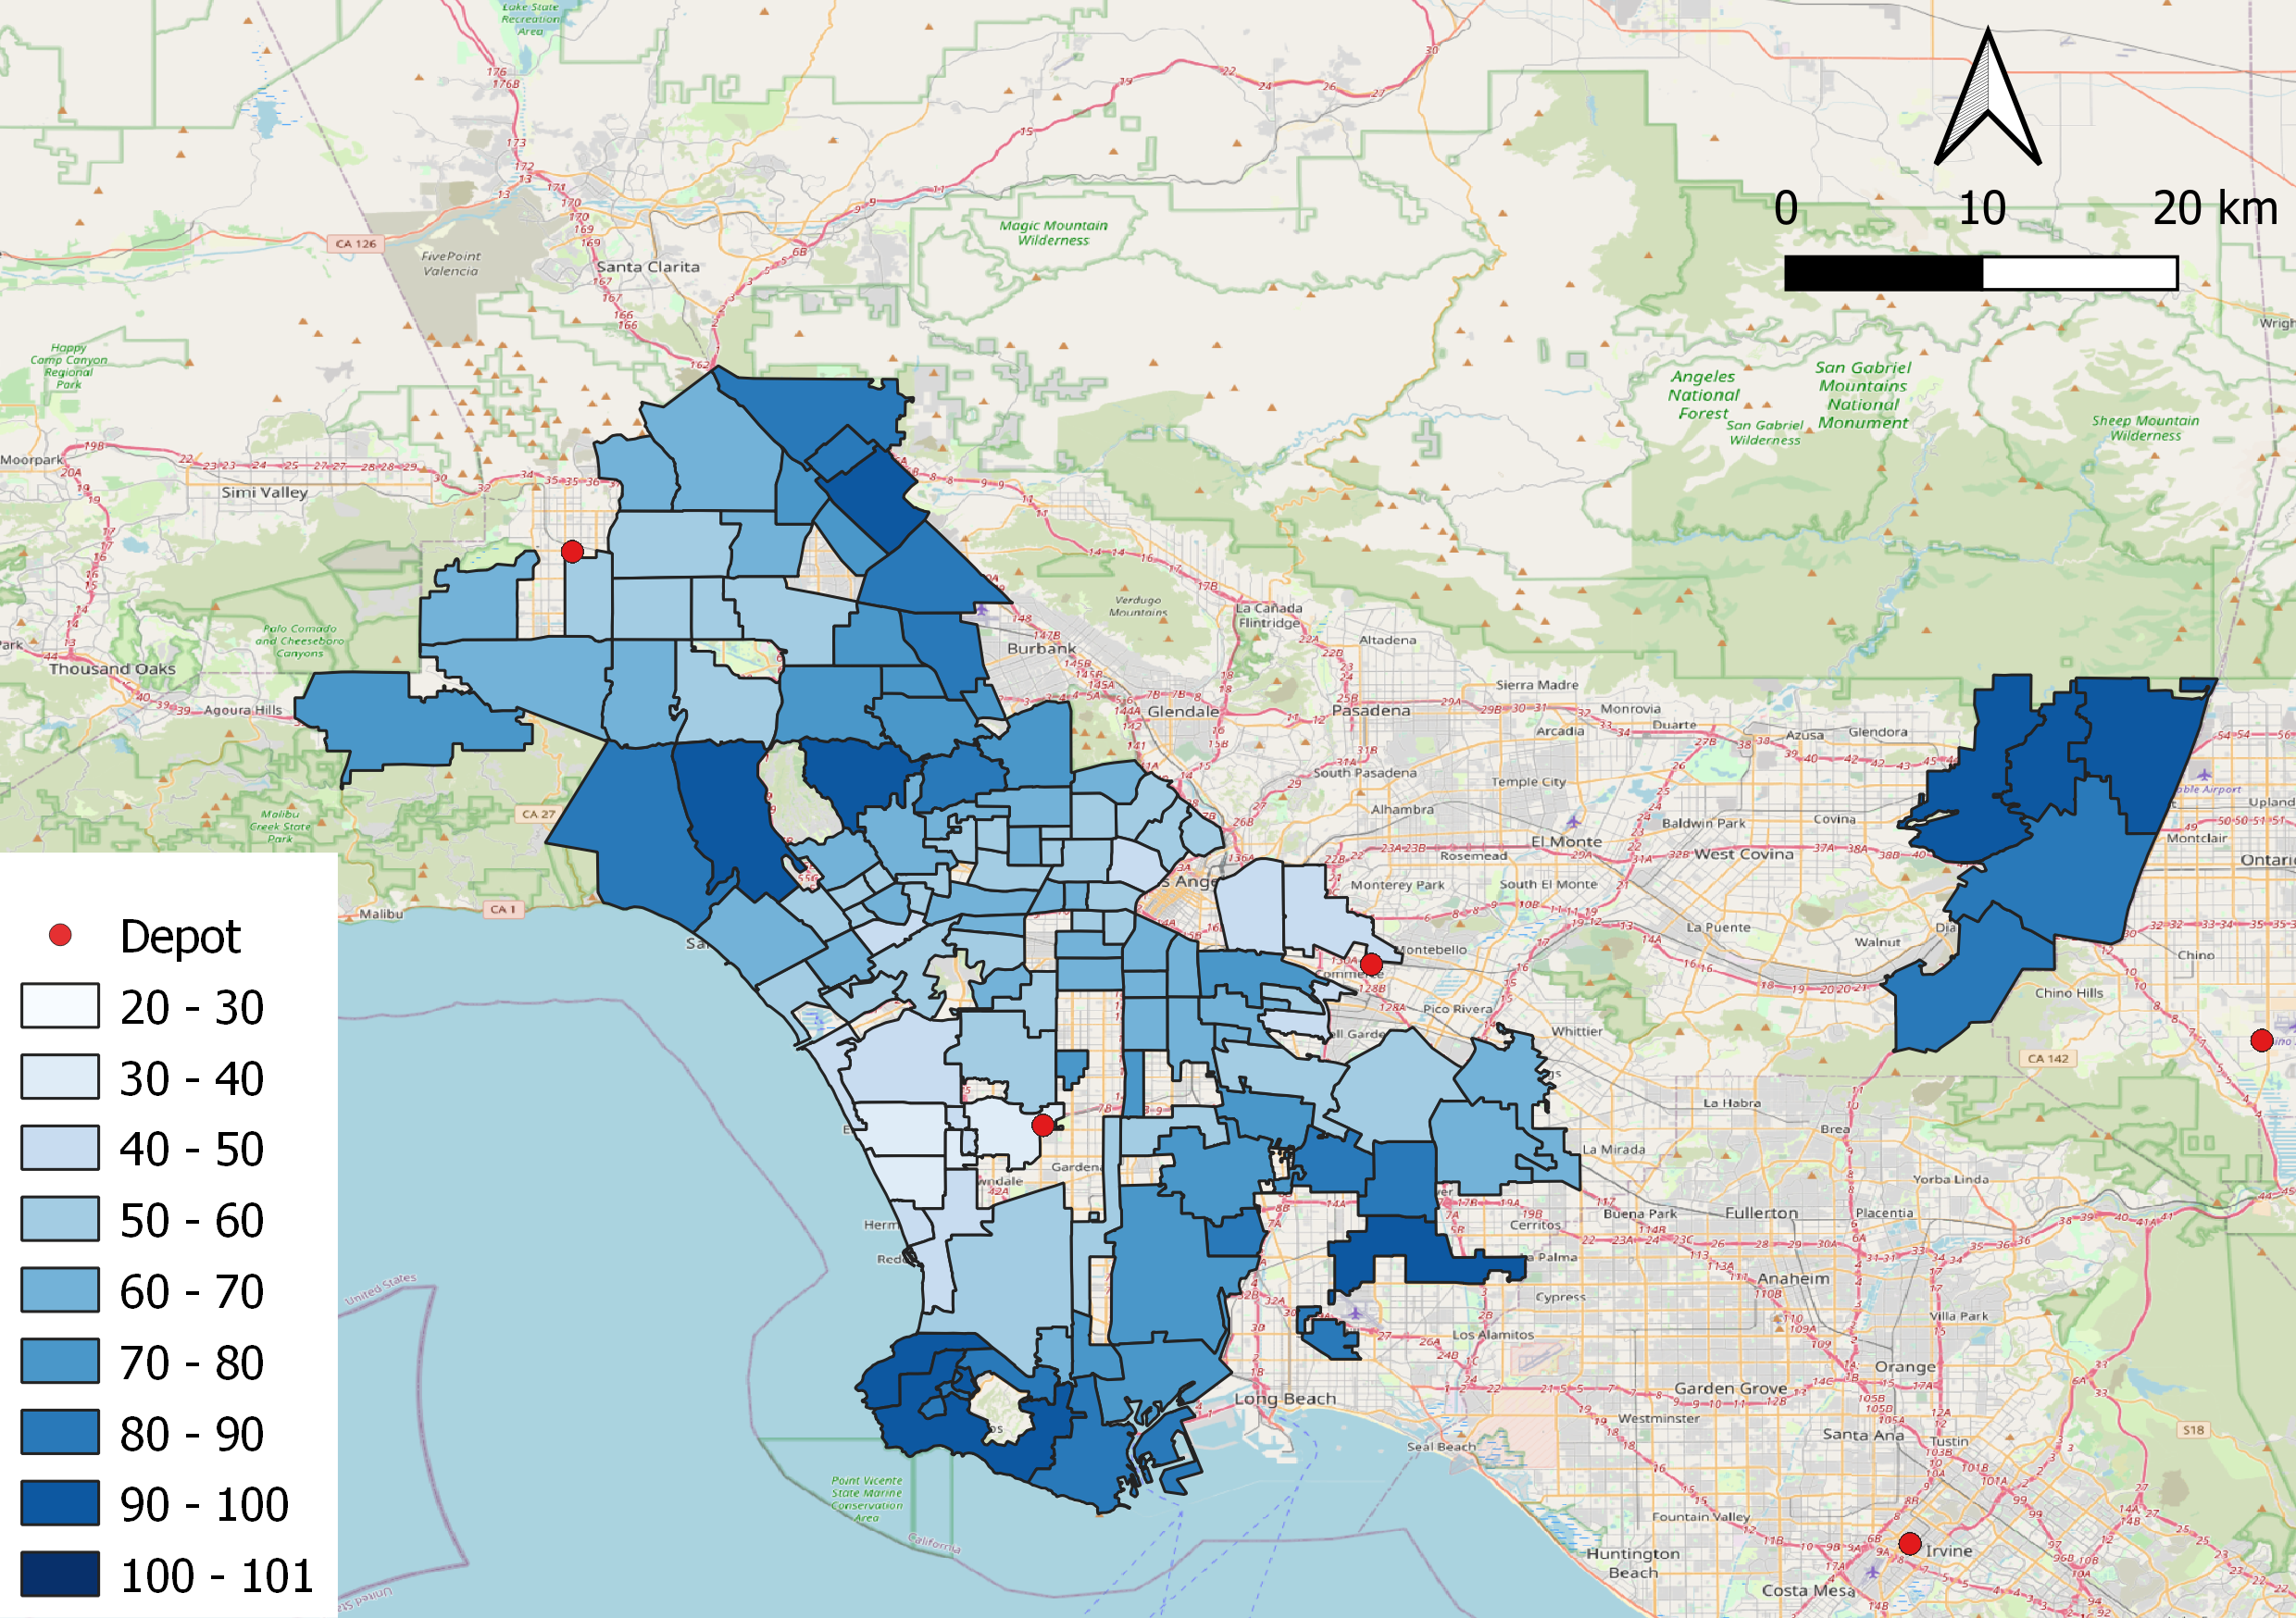
\includegraphics[width=\textwidth]{images/6_amazon/distancias/Avg Sum of Driving Dist. Route - LA.png}
    \end{subfigure}
    \caption*{\ Fonte: Produzido pelos autores Fernandes \& Alves}
\end{figure}

A Figura \ref{fig:fc_medio_LA} apresenta os valores médios de fator de circuito por bairros de Los Angeles.
A princípio, não é possível identificar qualquer padrão ou consistência na distribuição espacial apresentada

\begin{figure}[H]
    \centering
    \caption{Fator de circuito médio nos bairros de Los Angeles (\textit{Amazon})}
    \label{fig:fc_medio_LA}
    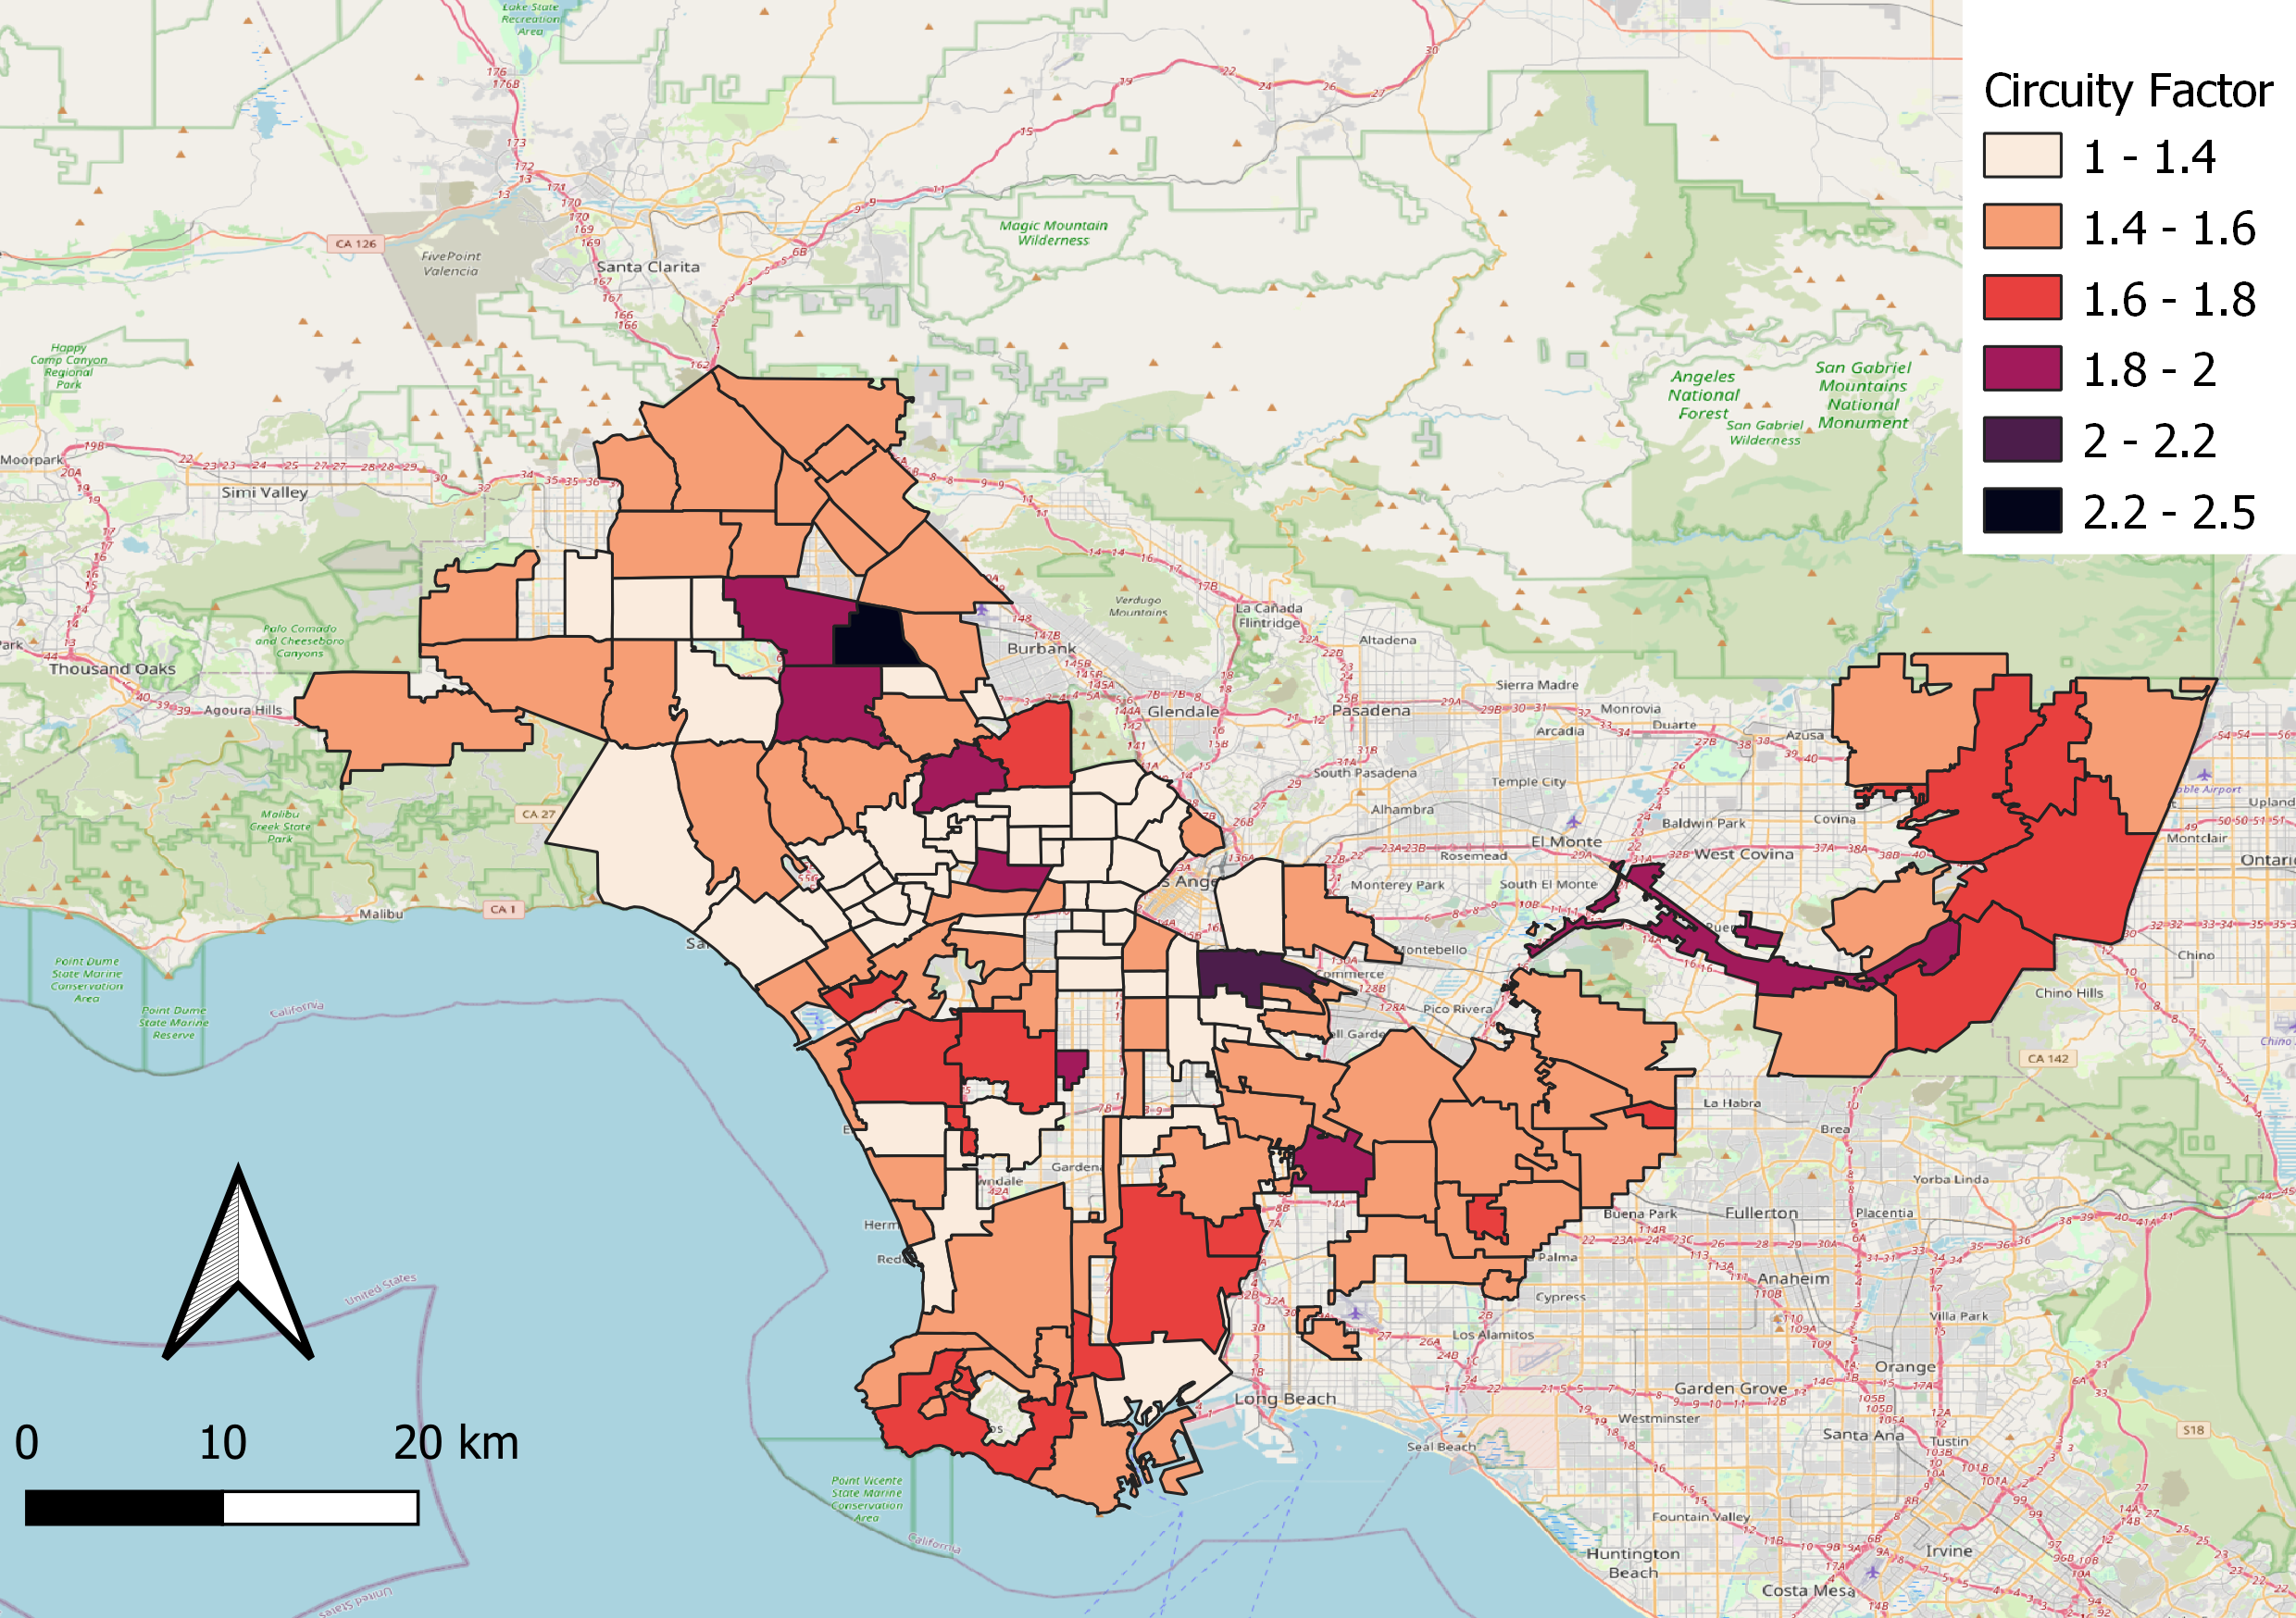
\includegraphics[width=0.55\textwidth]{images/6_amazon/fc/fc_la_avvg_per_stop.png}
    \caption*{\ Fonte: Produzido pelos autores Fernandes \& Alves}
\end{figure}

%%%%%%%%%%%%%%%%%%%%%%%%%%%%%%%%%
\section{Análise da malha viária} \label{sec:Amazon_MalhaViaria}

A análise da geometria de malha viária foi realizada para as cinco cidades estudadas, gerando uma elevada quantidade de informações relativas à densidade e à conectividade.
Um desafio enfrentado foi selecionar o melhor modelo para apresentar os resultados neste documento, visto que tratam-se de cento e oitenta bairros somente na cidade de Los Angeles, sem contar os bairros das outras cinco cidades.
Sendo assim, serão apresentados nesta Seção apenas resumos dos resultados obtidos, sendo os resultados completos apresentados ou nos apêndices ou no repositório publicado por \citeonline{guilherme_fernandes_alves_2022_6792977} na plataforma \textit{github}.

A Figura \ref{fig:graphsLosAngeles} apresenta exemplo dos grafos gerados para a cidade de Los Angeles, onde os pontos azuis representam os nós e as linhas pretas representam os arcos.
É possível notar que o modelo utilizado considera diferentes arcos para compor uma mesma rua, de modo a reduzir o número de arcos curvilíneos no grafo.

\begin{figure}[H]
    \centering
    \caption{Exemplos de grafos gerados para os bairros de Los Angeles (\textit{Amazon})} \label{fig:graphsLosAngeles}
    %
    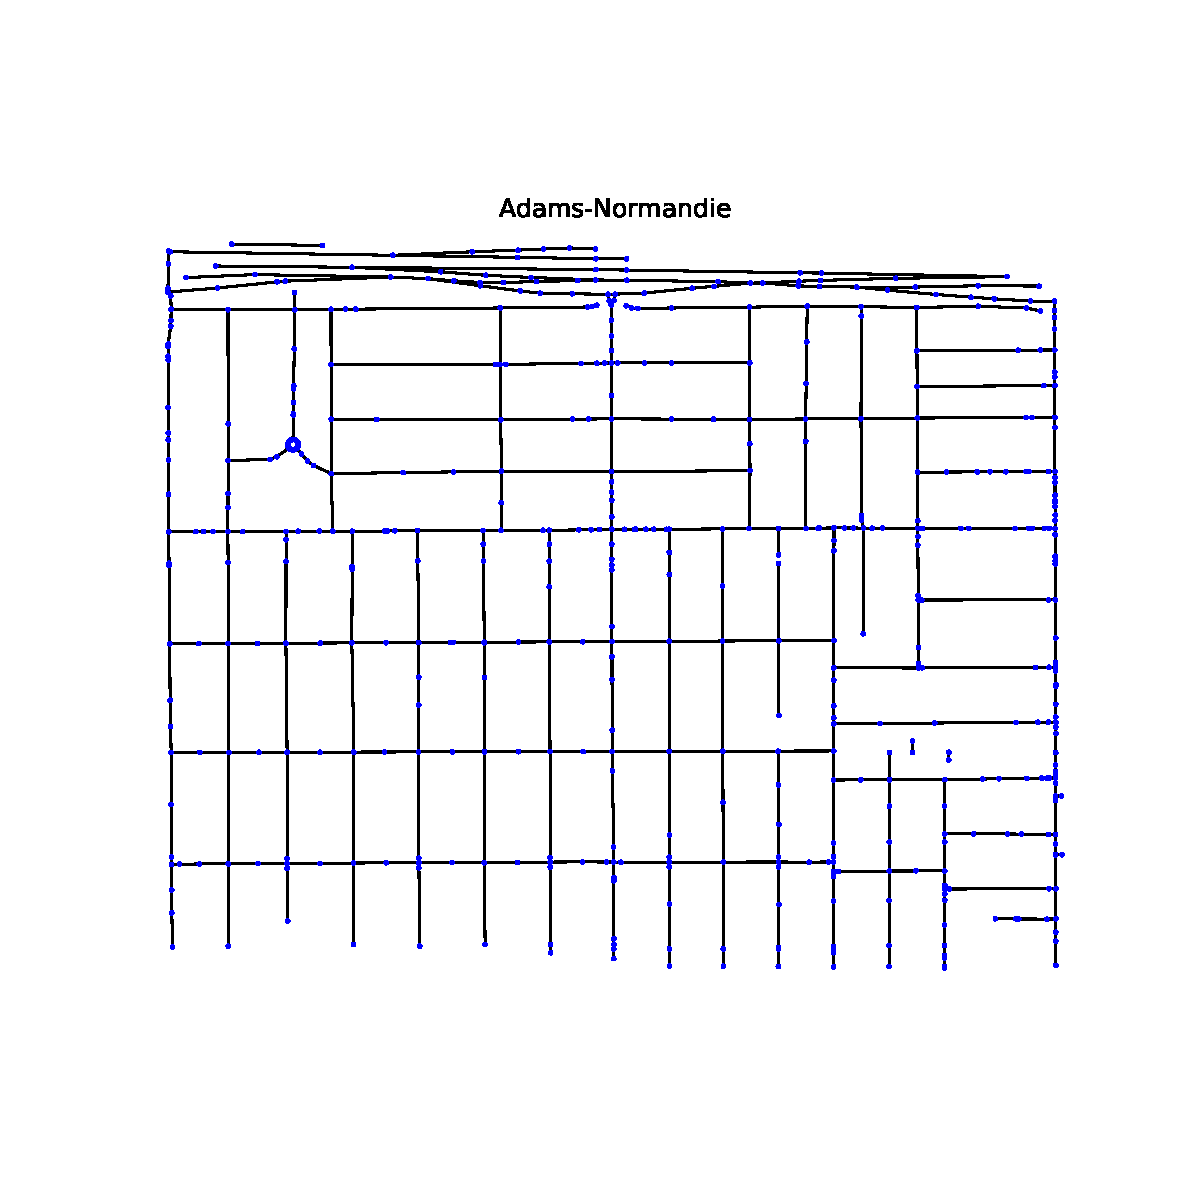
\includegraphics[width=0.48\textwidth]{images/6_amazon/grafos/graph_Adams-Normandie.pdf}
    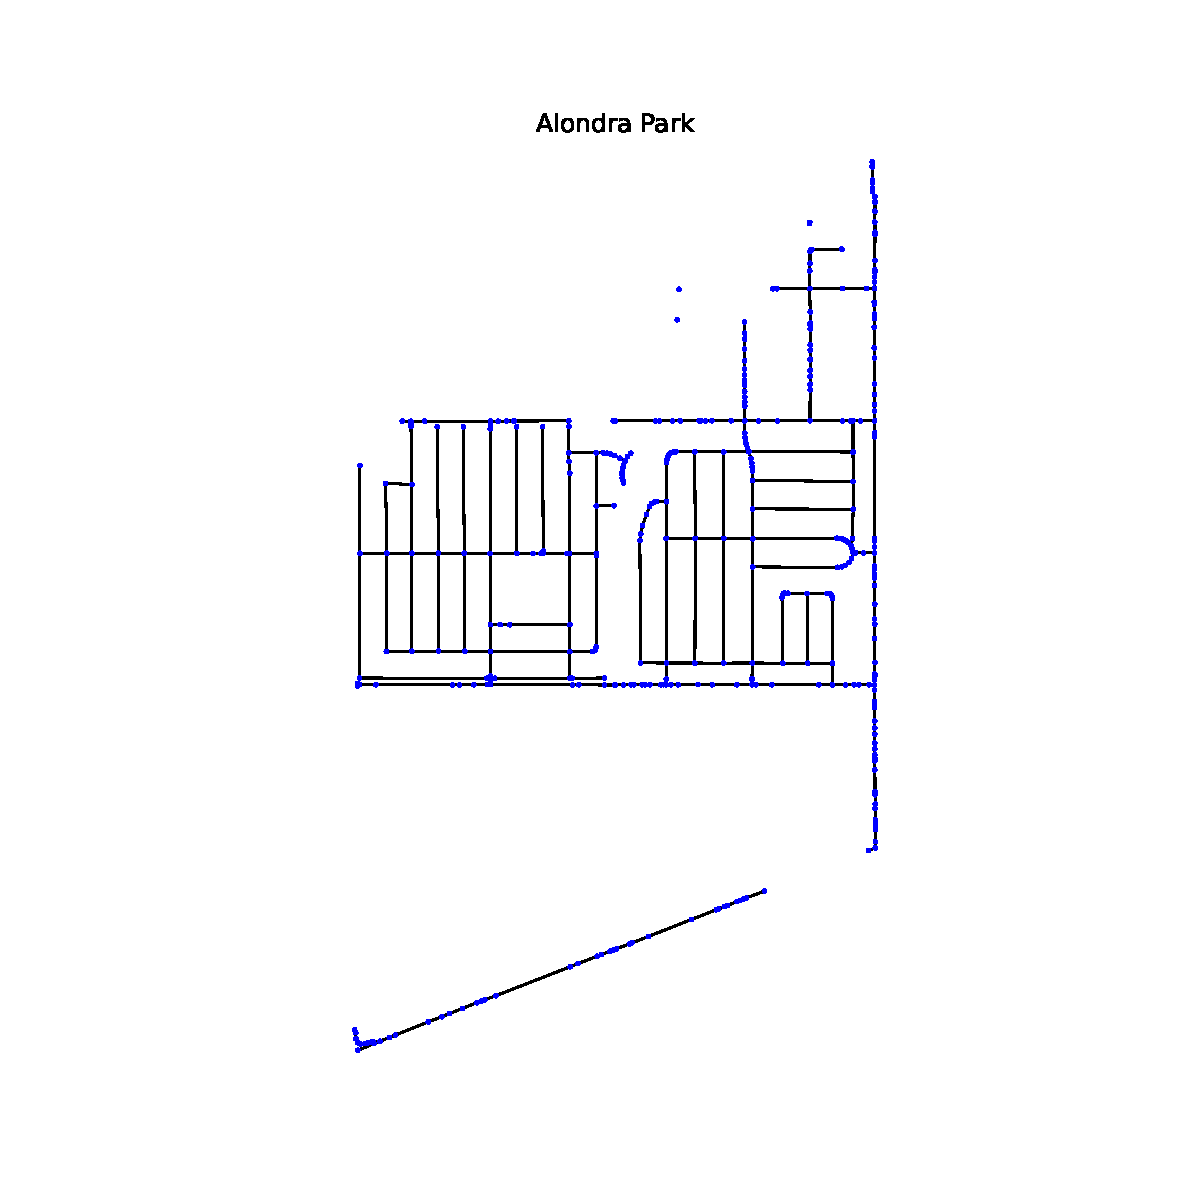
\includegraphics[width=0.48\textwidth]{images/6_amazon/grafos/graph_Alondra Park.pdf}
    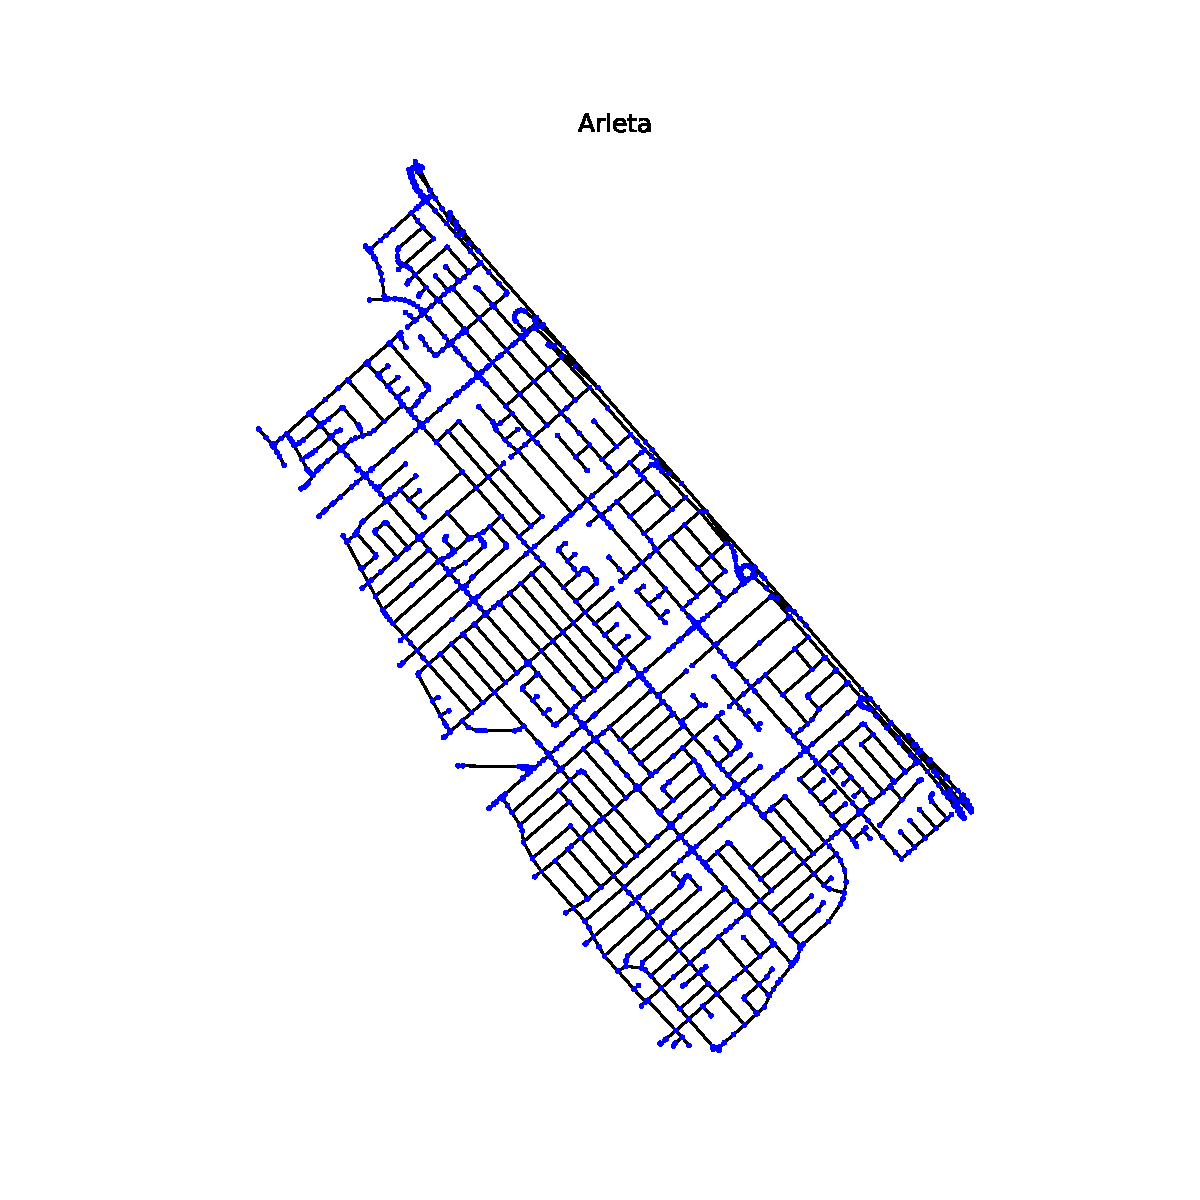
\includegraphics[width=0.48\textwidth]{images/6_amazon/grafos/graph_Arleta.pdf}
    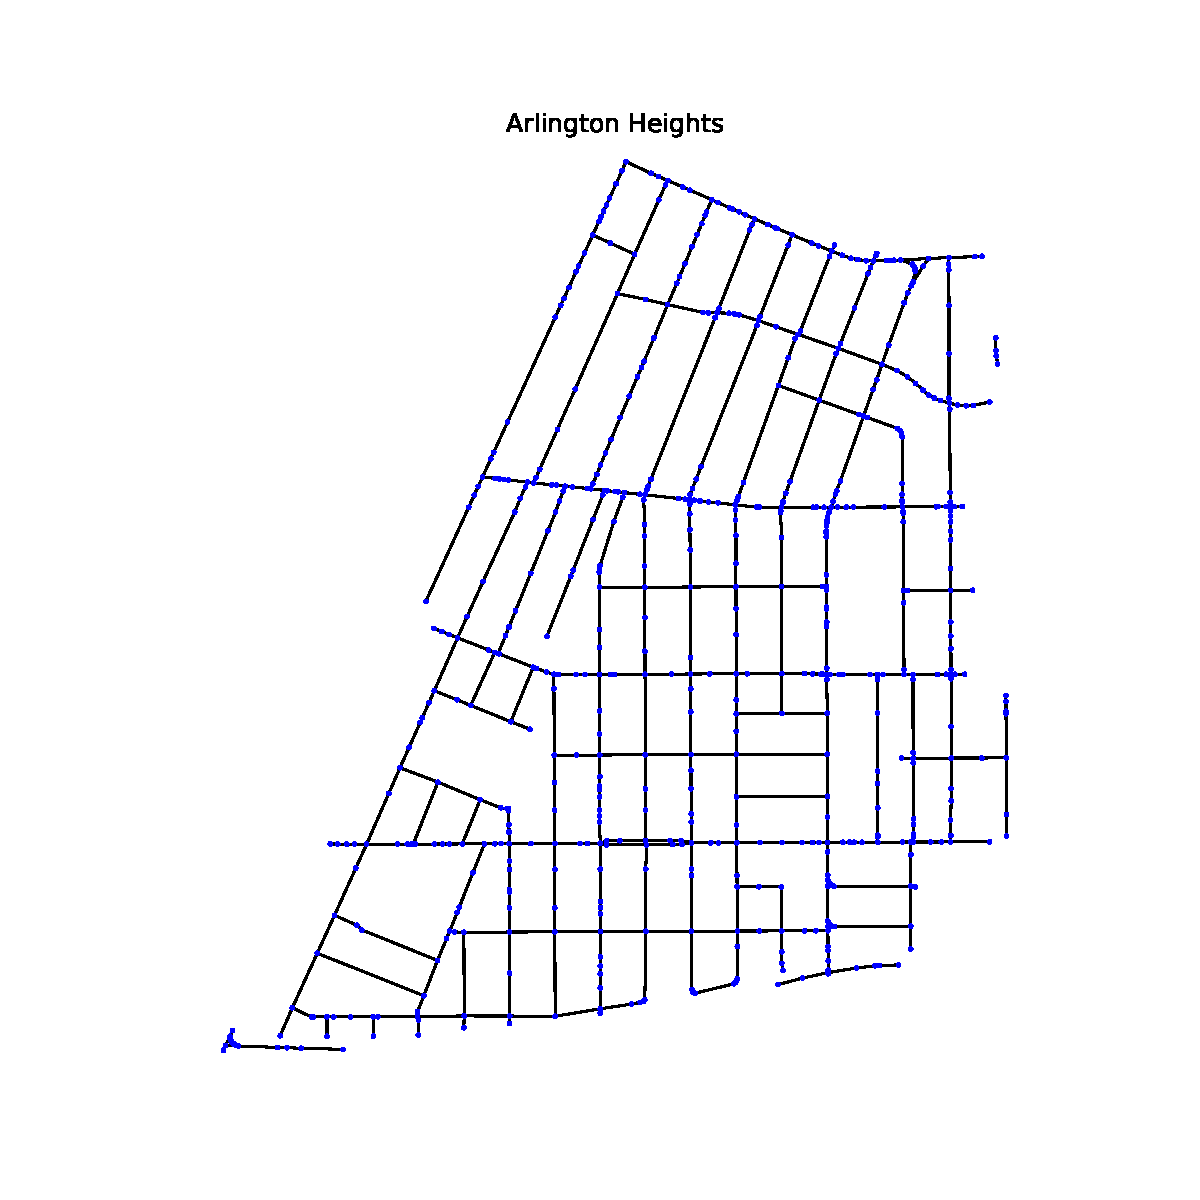
\includegraphics[width=0.48\textwidth]{images/6_amazon/grafos/graph_Arlington Heights.pdf}
    %
    \caption*{Fonte: Produzido pelos autores Fernandes \& Alves}
\end{figure}

A partir dos grafos, primeiramente foram calculadas as estatísticas básicas permitidas pela biblioteca \textit{OSMnx}.
A Tabela \ref{tab:basic_stats_LA} apresenta o resumo dessas estatísticas para a cidade de Los Angeles. 
As linhas da Tabela estão ordenadas em ordem alfabética pelo nome dos bairros.

\singlespacing
\begin{table}[H]
    \centering
    \caption{Estatísticas geradas para Los Angeles}
    \label{tab:basic_stats_LA}
    \resizebox{\textwidth}{!}{%
    \begin{tabular}{|llllllll|}
    \hline
    \multicolumn{1}{|l|}{\textbf{id}} & \multicolumn{1}{l|}{\textbf{Neighborhood}} & \multicolumn{1}{l|}{\textbf{n}} & \multicolumn{1}{l|}{\textbf{m}} & \multicolumn{1}{l|}{\textbf{k\_avg}} & \multicolumn{1}{l|}{\textbf{edge\_length\_total}} & \multicolumn{1}{l|}{\textbf{streets\_per\_node\_avg}} & \multicolumn{1}{l|}{\textbf{intersection\_count}} \\ \hline
    1 & Adams-Normandie & 527 & 1092 & 4.144 & 62956.846 & 2.343 & 513 \\
    2 & Alondra Park & 376 & 786 & 4.181 & 47819.489 & 2.239 & 364 \\
    3 & Arleta & 1371 & 2920 & 4.26 & 195960.705 & 2.28 & 1283 \\
    4 & Arlington Heights & 636 & 1379 & 4.336 & 66627.8 & 2.3 & 626 \\
    5 & Artesia & 1045 & 1875 & 3.589 & 94343.737 & 2.215 & 972 \\
    6 & Baldwin Hills/Crenshaw & 2392 & 4680 & 3.913 & 155618.547 & 2.138 & 2347 \\
    ... & ... & ... & ... & ... & ... & ... & ... \\
    174 & Whittier & 7040 & 14110 & 4.009 & 690578.884 & 2.226 & 6685 \\
    175 & Willowbrook & 1947 & 3830 & 3.934 & 213449.386 & 2.263 & 1870 \\
    176 & Wilmington & 3913 & 7838 & 4.006 & 377052.158 & 2.246 & 3831 \\
    177 & Windsor Square & 347 & 788 & 4.542 & 44654.552 & 2.395 & 347 \\
    178 & Winnetka & 3593 & 7509 & 4.18 & 293357.636 & 2.152 & 3401 \\
    179 & Woodland Hills & 11304 & 22709 & 4.018 & 675446.793 & 2.097 & 10956 \\\hline
    \end{tabular}%
    }
    \caption*{Fonte: Produzido pelos autores Fernandes \& Alves}
\end{table}
\onehalfspacing

%% Densidade e conectividade 
A partir das estatísticas iniciais, foi possível analisar a distribuição espacial da densidade e conectividades das malhas viárias associadas aos bairros das cidades. 
A Figura \ref{fig:conectividadeLA} apresenta a média de arcos conectados em cada nó presente nos bairros de Los Angeles ($k_{avg}$), do qual destaca-se que a região central da cidade concentra os bairros de maior conectividade.
A Figura \ref{fig:densidade_intersec} apresenta a densidade de intersecções ($D_{Intersec}$).
No geral, é possível notar que bairros em regiões mais centrais da cidade tendem a apresentar maior densidade de intersecções, seja pela maior presença de vias ou pela menor área que estes bairros apresentam. 

\begin{figure}[H]
    \centering
    \caption{Densidade e conectividade dos bairros da cidade de Los Angeles (\textit{Amazon})} 
    \begin{subfigure}{0.49\textwidth} 
        \caption{\textit{Node degree} ($k_{avg}$)} \label{fig:conectividadeLA}
        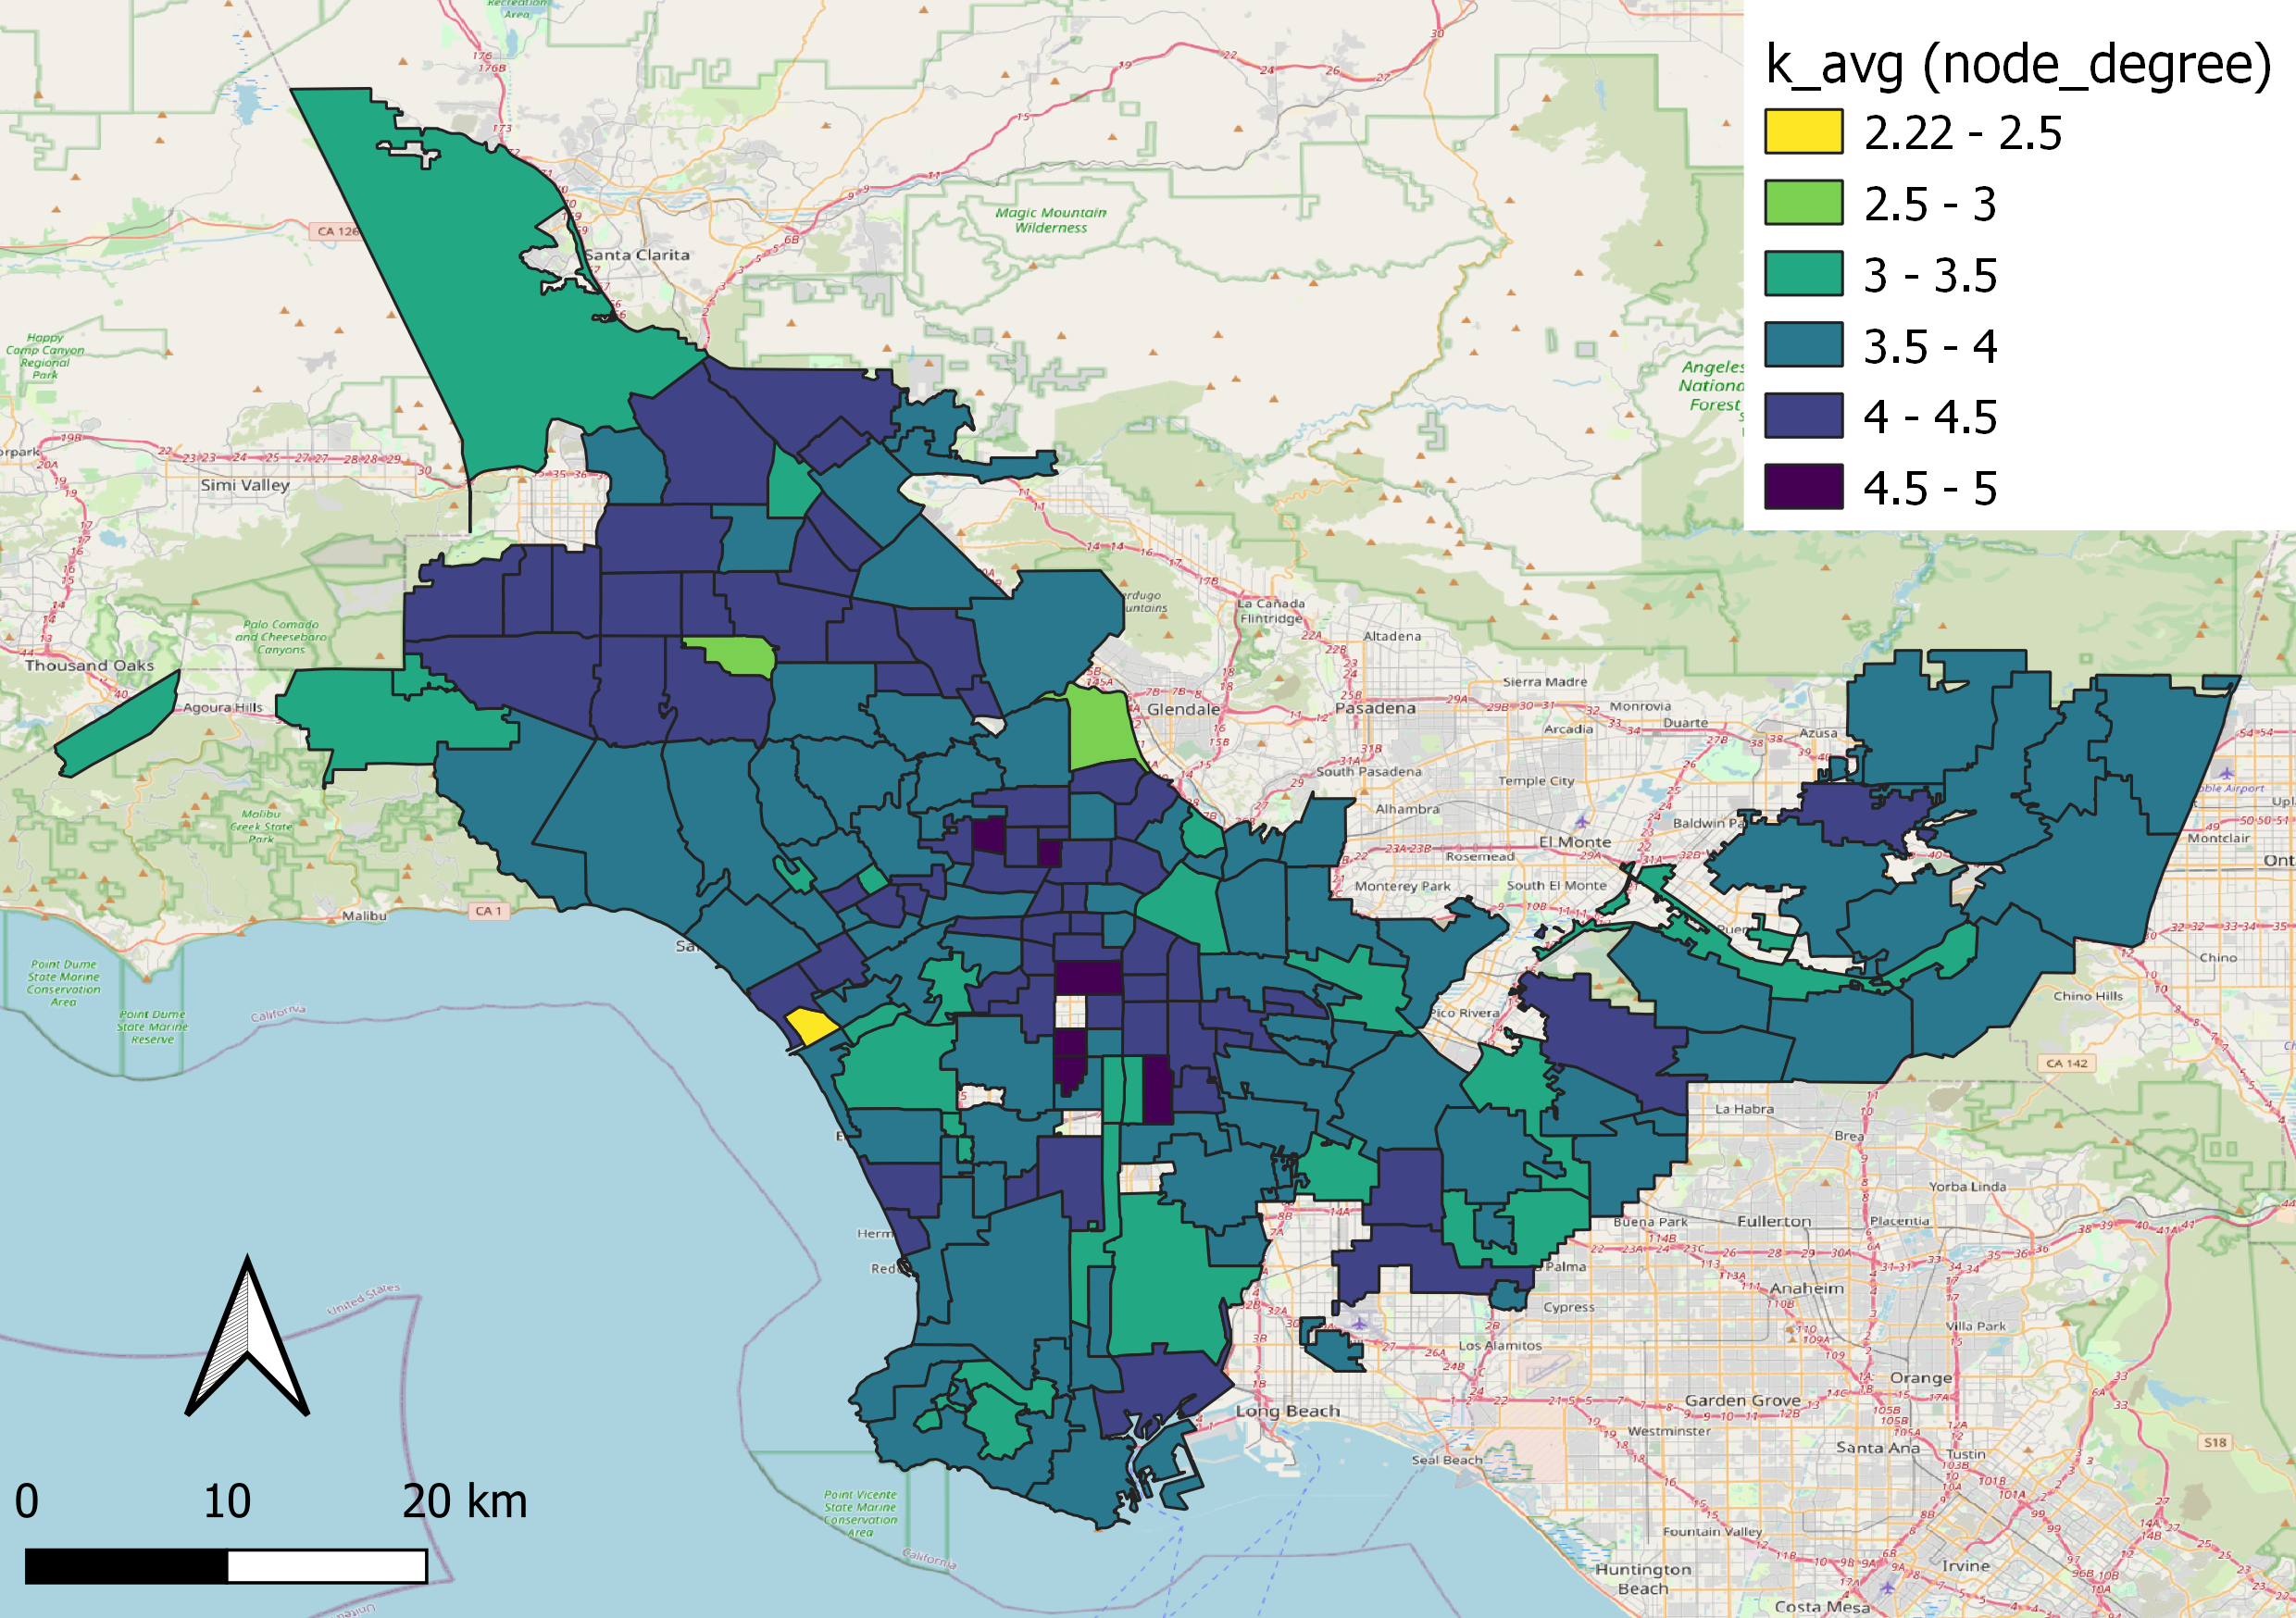
\includegraphics[width=\textwidth]{images/6_amazon/conectividade/k_avg.png}
    \end{subfigure}
    \begin{subfigure}{0.49\textwidth}
        \caption{Densidade de Intersecções ($D_{intersec}$)} \label{fig:densidade_intersec}
        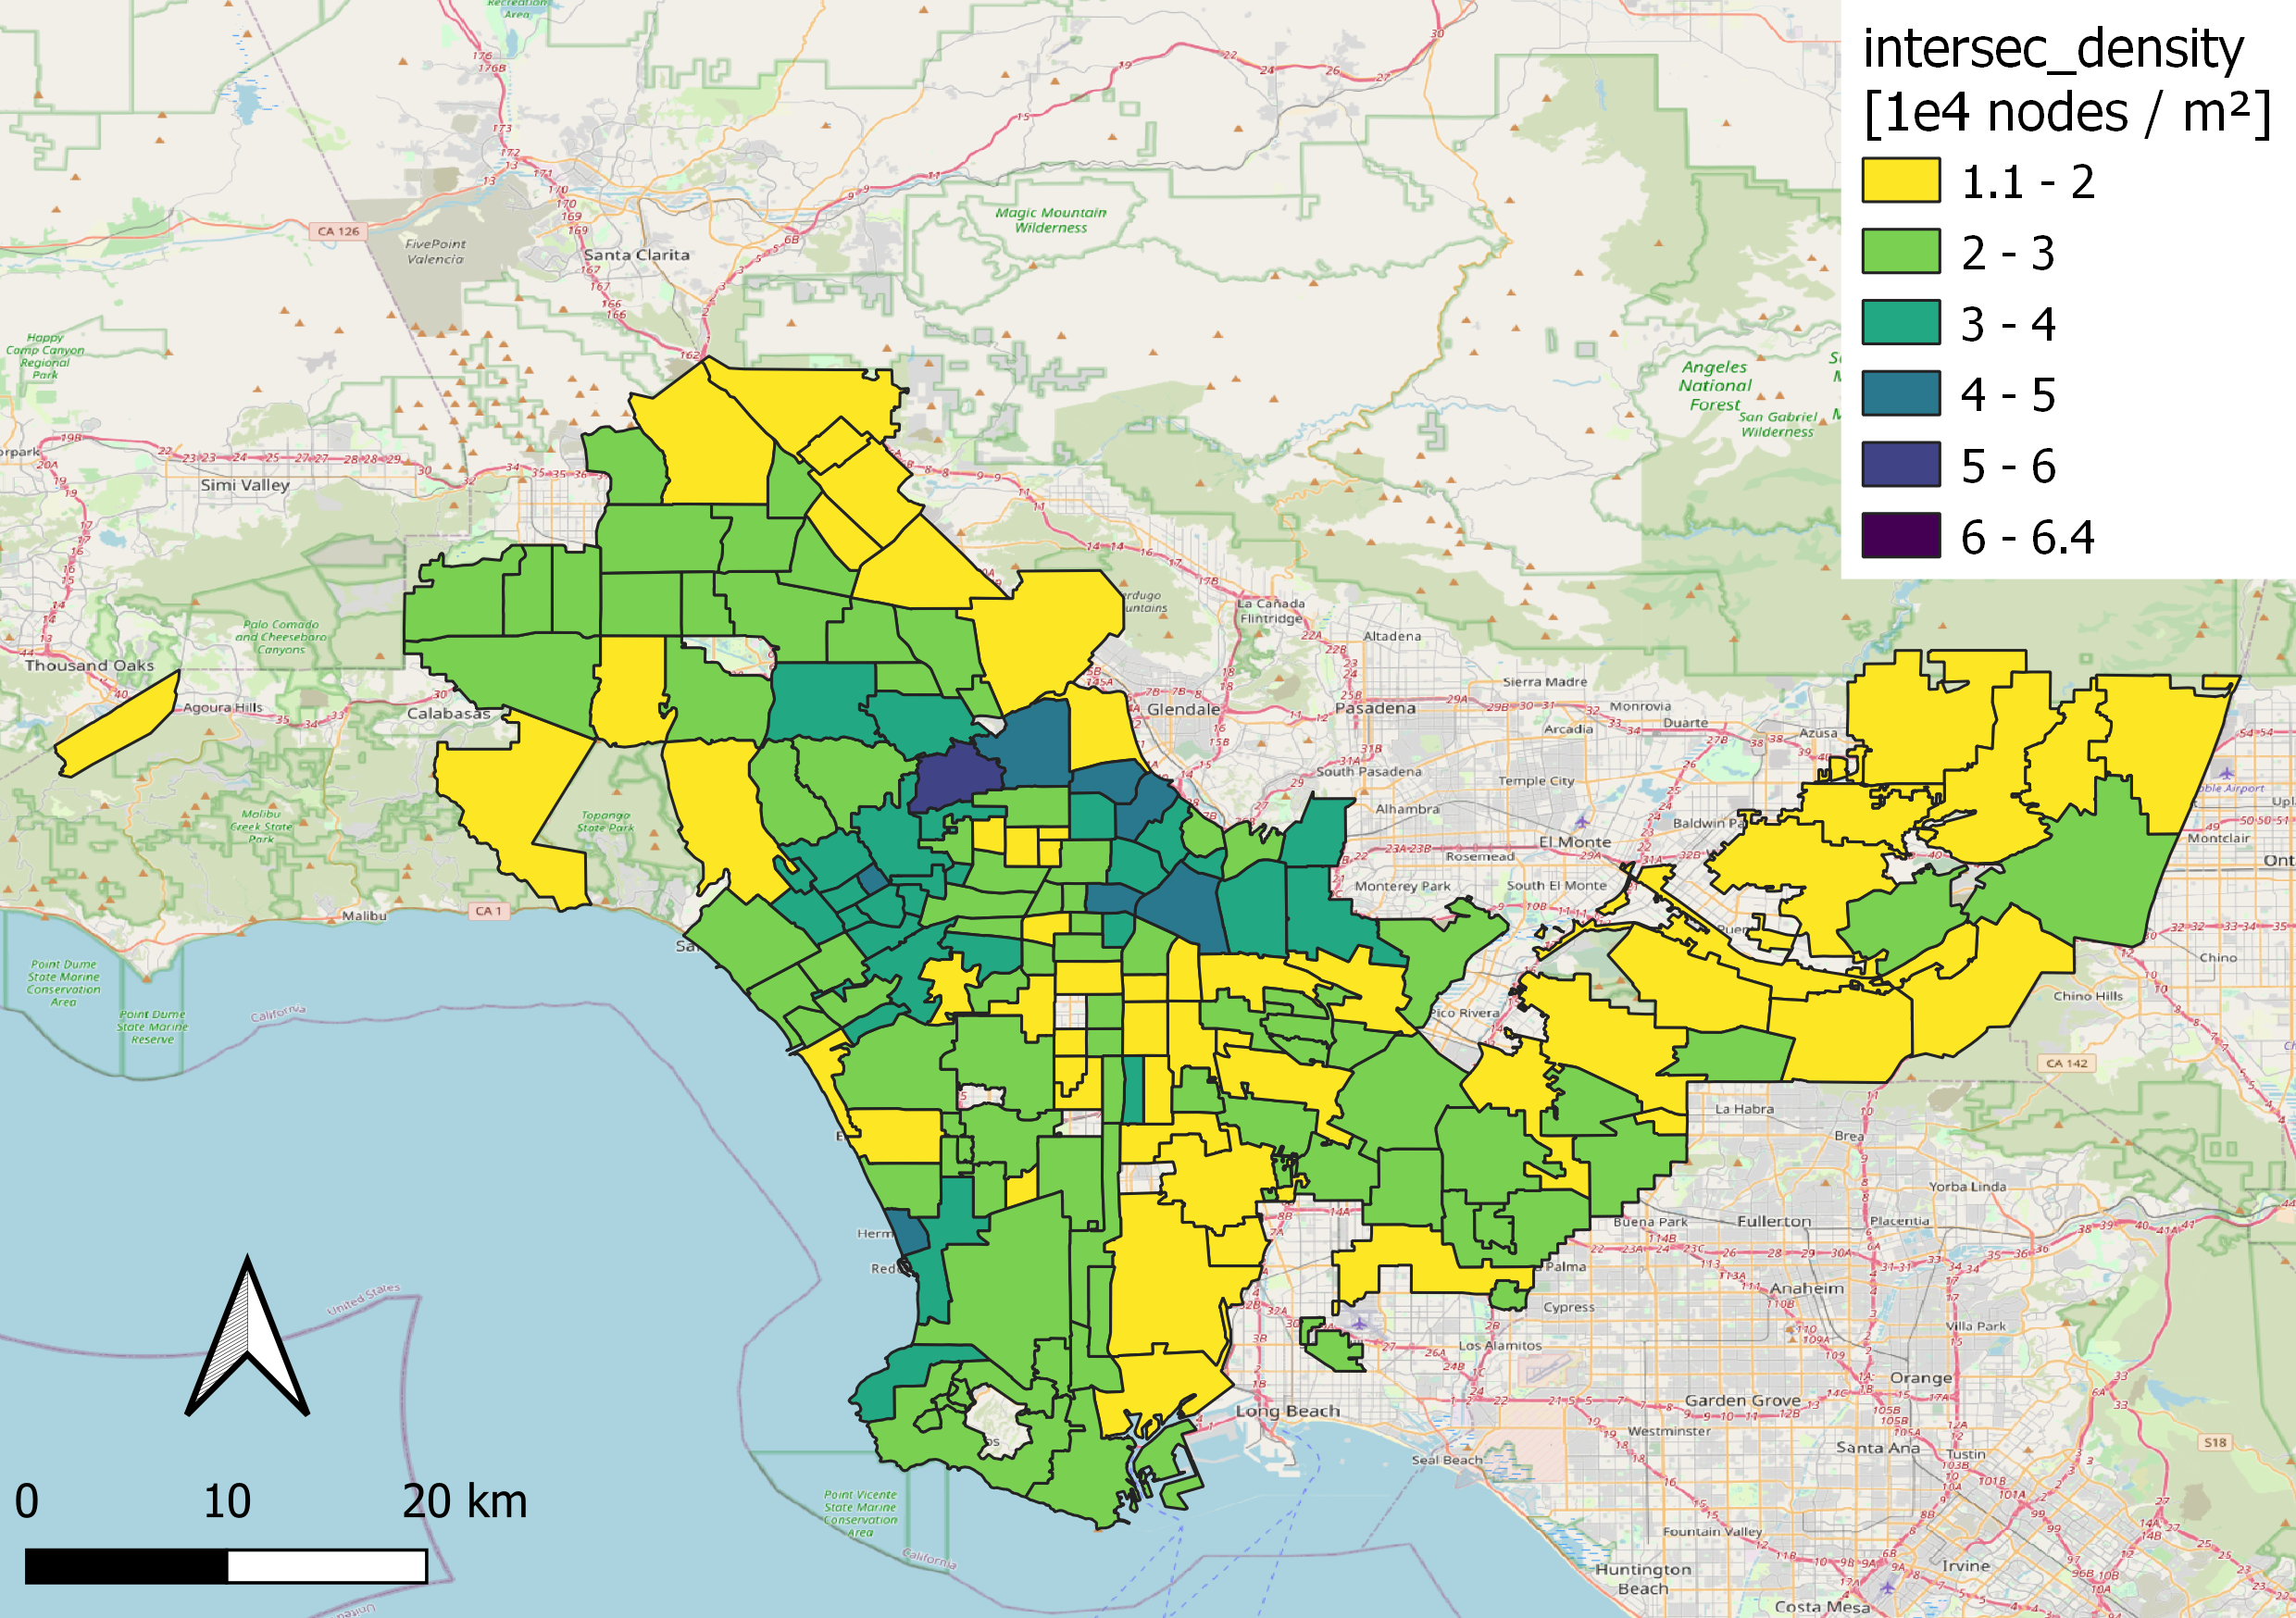
\includegraphics[width=\textwidth]{images/6_amazon/conectividade/la_intersec_density.png}
    \end{subfigure}
    \caption*{Fonte: Produzido pelos autores Fernandes \& Alves}
\end{figure}

%%%%%%%%%%%%%%%%%%%%%%%%%%%%%%%
% \subsection{Orientação de vias}
Também foi realizada a análise de orientações das vias dos bairros das cinco cidades analisadas.
A Figura \ref{fig:OrientacaoLosAngeles} exemplifica os histogramas polares de alguns dos bairros de Los Angeles.
A variável $\delta$, que aparece nas imagens presentes na Figura, representa o indicador $quadratic\_sum\_deviation$, que quantifica a variação do histograma. 
Quanto mais próximo de zero, mais a malha tende a não apresenta nenhuma direção predominante.
É a partir de $\delta$ que foi possível ordenar os histogramas em ordem de uniformidade, ou seja, ordenar os grafos em termos do quão organizadas - em termos de orientação - estão os seus arcos. 
Ressalta-se que uma série de indicadores foram calculados em adição aos indicadores que já estavam presentes no pacote \textit{OSMnx}, conforme descrito na Seção \ref{sec:aprofund-LMR}.

\begin{figure}[H]
    \centering
    \caption{Exemplo de orientação de vias nos bairros de Los Angeles. O ângulo representa o azimute das vias e a amplitude representa a contagem do número de vias. Intervalos de 10 graus.} \label{fig:OrientacaoLosAngeles}
    %
    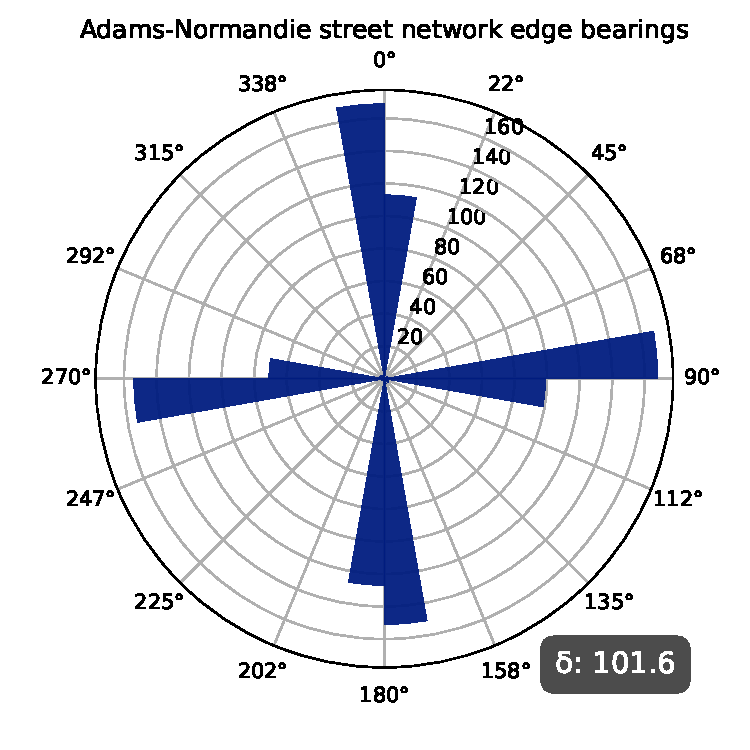
\includegraphics[width=0.48\textwidth]{images/6_amazon/orientacao/172 - polar_hist_street_orientation_Adams-Normandie.pdf}
    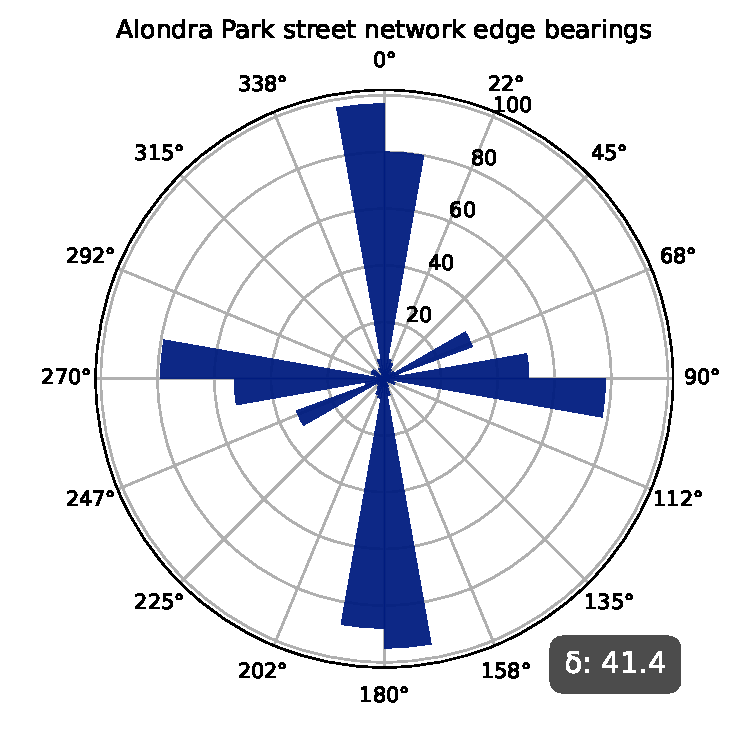
\includegraphics[width=0.48\textwidth]{images/6_amazon/orientacao/115 - polar_hist_street_orientation_Alondra Park.pdf}
    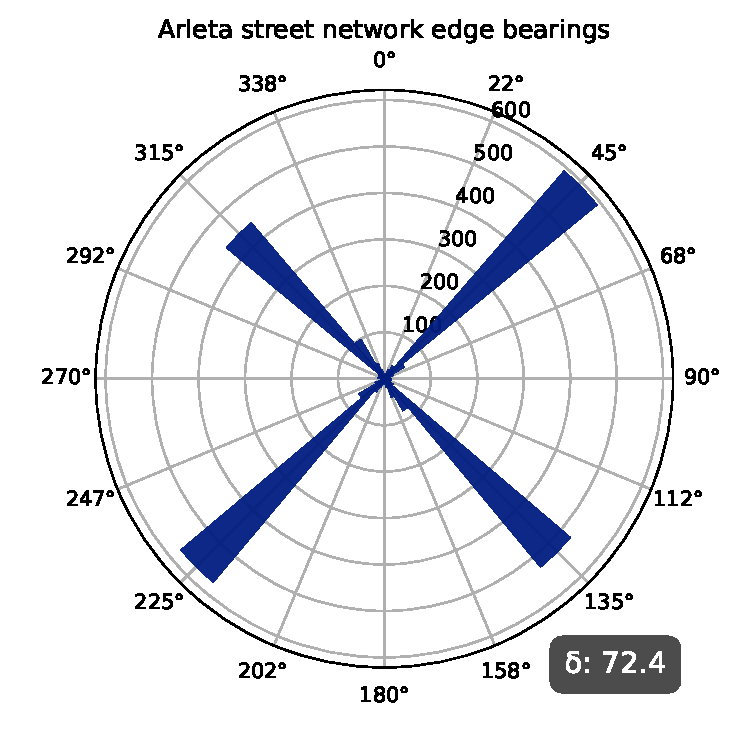
\includegraphics[width=0.48\textwidth]{images/6_amazon/orientacao/155 - polar_hist_street_orientation_Arleta.pdf}
    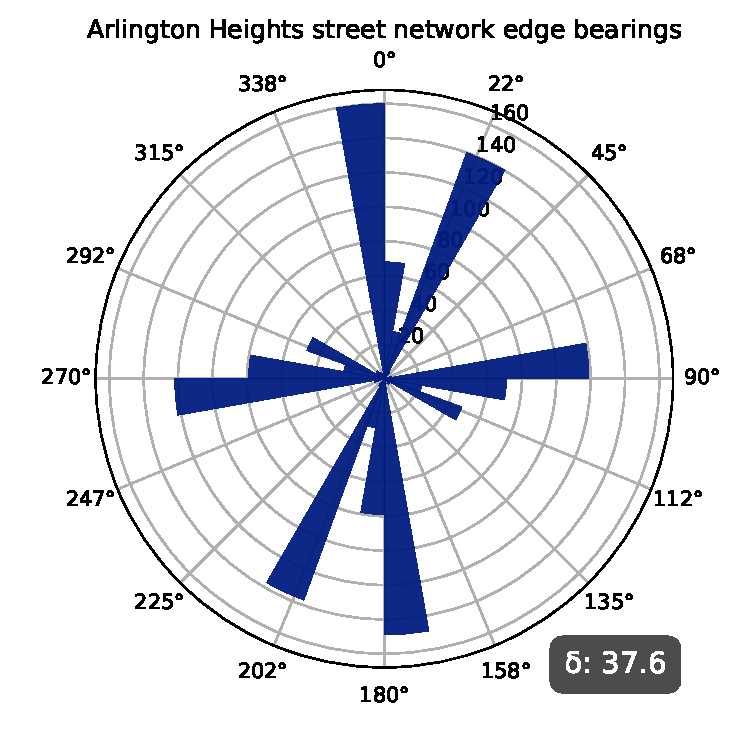
\includegraphics[width=0.48\textwidth]{images/6_amazon/orientacao/104 - polar_hist_street_orientation_Arlington Heights.pdf}
    %
    \caption*{Fonte: Produzido pelos autores Fernandes \& Alves}
\end{figure}


%%%%%%%%%%%%%%%%%%%%%%%%%%%%%%%%%%%%%%%%%%%%
\section{Relação entre as medidas estudadas}

%%%%%%%%%%%%%%%%%%%%%%%%%%%%%%%%%%%%%%%%%%%%%%%%%%%
\subsection{Fator de circuito e repasses}

%Assim como feito para o estudo de caso anterior, 
Primeiramente, é possível comparar o percentual de repasses com a média de fator de circuito dos bairros da cidade de Los Angeles. 
Tal comparação pode ser visualizada na Figura \ref{fig:fc_regressao_LA}.
Nota-se um efeito contraditório em que o percentual de repasses é maior para os bairros que possuem menor média de fator de circuito.
Ainda assim, o valor do coeficiente de determinação da regressão presente na Figura é relativamente pequeno, não permitindo que o modelo seja utilizado para explicar a variação presente na amostra. 
Uma regressão cúbica foi selecionada de modo a maximizar o ajuste dos dados.

\begin{figure}[H]
    \centering
    \caption{Percentual de repasses em função do fator de circuito médio nos bairros de Los Angeles (\textit{Amazon})}
    \label{fig:fc_regressao_LA}
    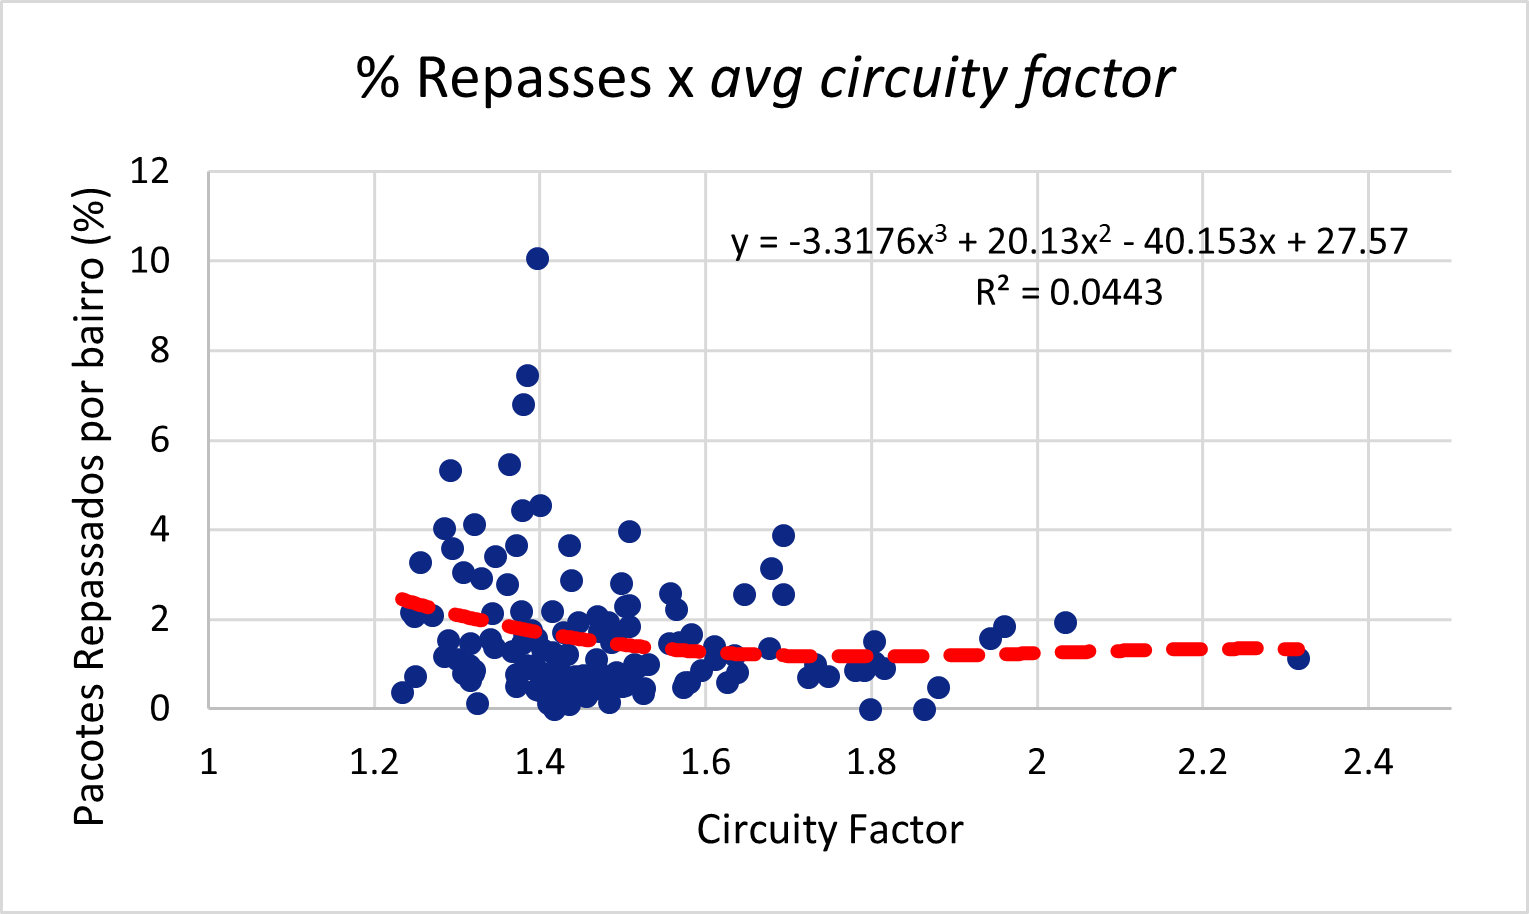
\includegraphics[width=0.6\textwidth]{images/6_amazon/fc/repasses_x_cf_la.png}
    \caption*{\ Fonte: Produzido pelos autores Fernandes \& Alves}
\end{figure}


%%%%%%%%%%%%%%%%%%%%%%%%%%%%%%%%%%%%%%%%%%%%%%%%%%%%%%%%%%%%%%%
\subsection{Regressões simples} \label{CorrelacaoPreditorUnico}

% Após a construção de todos os indicadores para cada bairro, estes foram compilados em uma única base de dados bairro a bairro junto às informações de repasse e devolução.
% Em sequência, as variáveis de contagem e extensão total foram normalizadas pelas áreas respectivas de cada bairro para que o efeito dos diferentes tamanhos dos bairros seja neutralizado.

A fim de se conseguir regressões lineares entre os pares de variáveis obtidos anteriormente, inicialmente retirou-se da análise bairros pouco representativos estatisticamente. 
Para tal, utilizando-se o conceito de representatividade amostral (\citeauthoronline{medri2011analise}, \citeyear{medri2011analise}), adota-se que cada bairro representa de uma amostra da população total de $144411$ entregas analisadas em Los Angeles.
Assim, assumindo-se um erro amostral tolerável de $5\%$, o tamanho mínimo amostral é de aproximadamente 400 pontos. 
Dessa forma, retirou-se da análise os 75 bairros com menos de 400 pontos de entrega qualificados como pouco representativos.

Com os noventa bairros restantes, calculou-se o coeficiente de correlação entre os indicadores de devolução, repasse e os indicadores de malha. 
Os resultados podem ser observados na Tabela \ref{tab:correlacao_AMAZON}, que contém uma matriz de correlação dessas variáveis.

\begin{spacing}{1}
\begin{table}[htb] 
    \centering
    \caption{Matriz de correlação entre repasses, devoluções e os indicadores de malha, considerando apenas a cidade de Los Angeles (\textit{Amazon})}
    \label{tab:correlacao_AMAZON}
    \resizebox{\textwidth}{!}{\begin{tabular}{|c|ccc|ccc|}%{|c|cC{1.3cm}C{1.3cm}|C{1.3cm}C{1.3cm}C{1.3cm}|}
    \hline
    {\color[HTML]{4472C4}} & \cellcolor[HTML]{4472C4}{\color[HTML]{FFFFFF} Nº Repasse} & \cellcolor[HTML]{4472C4}{\color[HTML]{FFFFFF} Nº Repasse / km²} & \cellcolor[HTML]{4472C4}{\color[HTML]{FFFFFF} Repasse (\%) } & \cellcolor[HTML]{4472C4}{\color[HTML]{FFFFFF} Nº Devolução} & \cellcolor[HTML]{4472C4}{\color[HTML]{FFFFFF} Nº Devolução / km²} & \cellcolor[HTML]{4472C4}{\color[HTML]{FFFFFF} Devolução (\%)} \\ \hline
    \textit{n} & \cellcolor[HTML]{EE6D62}0,06 & \cellcolor[HTML]{A69252}-0,36 & \cellcolor[HTML]{E1745E}-0,12 & \cellcolor[HTML]{EE6D62}0,06 & \cellcolor[HTML]{F56A62}-0,04 & \cellcolor[HTML]{F36B62}-0,05 \\
    \textit{n/km²} & \cellcolor[HTML]{A49352}0,33 & \cellcolor[HTML]{73AB48}0,50 & \cellcolor[HTML]{BD8658}0,24 & \cellcolor[HTML]{F16C63}0,05 & \cellcolor[HTML]{DB775E}0,13 & \cellcolor[HTML]{DA775E}0,13 \\
    \textit{m} & \cellcolor[HTML]{ED6E62}0,07 & \cellcolor[HTML]{A89152}-0,35 & \cellcolor[HTML]{E5725F}-0,10 & \cellcolor[HTML]{F06C62}0,05 & \cellcolor[HTML]{F56A63}-0,04 & \cellcolor[HTML]{F46B62}-0,04 \\
    \textit{m/km²} & \cellcolor[HTML]{A89153}0,31 & \cellcolor[HTML]{70AD47}0,51 & \cellcolor[HTML]{B98857}0,25 & \cellcolor[HTML]{F26B63}0,05 & \cellcolor[HTML]{D8785D}0,14 & \cellcolor[HTML]{D7795D}0,14 \\
    \textit{k\_avg} & \cellcolor[HTML]{FD6664}-0,01 & \cellcolor[HTML]{D57A5D}0,15 & \cellcolor[HTML]{D57A5D}0,15 & \cellcolor[HTML]{F66A63}-0,03 & \cellcolor[HTML]{F26B63}0,05 & \cellcolor[HTML]{F16C62}0,05 \\
    \textit{edge\_length\_total} & \cellcolor[HTML]{F06D62}-0,06 & \cellcolor[HTML]{969A4F}-0,42 & \cellcolor[HTML]{D67A5C}-0,16 & \cellcolor[HTML]{F76964}0,03 & \cellcolor[HTML]{F26C62}-0,05 & \cellcolor[HTML]{F16C62}-0,05 \\
    \textit{edge\_length\_total/km²} & \cellcolor[HTML]{E87061}0,08 & \cellcolor[HTML]{9C9751}0,36 & \cellcolor[HTML]{DA775E}0,13 & \cellcolor[HTML]{FC6665}0,01 & \cellcolor[HTML]{E0745F}0,11 & \cellcolor[HTML]{DF755F}0,12 \\
    \textit{edge\_length\_avg} & \cellcolor[HTML]{C48358}-0,24 & \cellcolor[HTML]{C68259}-0,23 & \cellcolor[HTML]{D9785D}-0,15 & \cellcolor[HTML]{EF6D61}-0,06 & \cellcolor[HTML]{F06D61}-0,06 & \cellcolor[HTML]{F06D61}-0,06 \\
    \textit{streets\_per\_node\_avg} & \cellcolor[HTML]{E0755E}-0,12 & \cellcolor[HTML]{EF6D62}0,06 & \cellcolor[HTML]{F76964}0,03 & \cellcolor[HTML]{F16C62}-0,05 & \cellcolor[HTML]{F66964}0,03 & \cellcolor[HTML]{F56A63}0,04 \\
    \textit{intersection\_count} & \cellcolor[HTML]{EC6E61}0,07 & \cellcolor[HTML]{A89152}-0,35 & \cellcolor[HTML]{E4735F}-0,11 & \cellcolor[HTML]{F06C62}0,06 & \cellcolor[HTML]{F56A63}-0,04 & \cellcolor[HTML]{F46B62}-0,04 \\
    \textit{intersection\_count/km²} & \cellcolor[HTML]{A49252}0,33 & \cellcolor[HTML]{71AC48}0,51 & \cellcolor[HTML]{BA8857}0,25 & \cellcolor[HTML]{F16C63}0,05 & \cellcolor[HTML]{DA785E}0,14 & \cellcolor[HTML]{D9785D}0,14 \\
    % \textit{street\_length\_total} & \cellcolor[HTML]{F06D62}-0,06 & \cellcolor[HTML]{979A4F}-0,42 & \cellcolor[HTML]{D57B5C}-0,17 & \cellcolor[HTML]{F46A63}0,04 & \cellcolor[HTML]{F26C62}-0,05 & \cellcolor[HTML]{F16C62}-0,05 \\
    % \textit{street\_length\_total/km²} & \cellcolor[HTML]{E87061}0,08 & \cellcolor[HTML]{A59252}0,32 & \cellcolor[HTML]{E0745F}0,11 & \cellcolor[HTML]{FB6765}0,02 & \cellcolor[HTML]{E3735F}0,10 & \cellcolor[HTML]{E2745F}0,11 \\
    % \textit{street\_segment\_count} & \cellcolor[HTML]{F06C62}0,05 & \cellcolor[HTML]{A59352}-0,36 & \cellcolor[HTML]{E1745E}-0,12 & \cellcolor[HTML]{F06C62}0,06 & \cellcolor[HTML]{F56A62}-0,04 & \cellcolor[HTML]{F36B62}-0,04 \\
    % \textit{street\_segment\_count/km²} & \cellcolor[HTML]{A99053}0,31 & \cellcolor[HTML]{72AC48}0,51 & \cellcolor[HTML]{BC8657}0,24 & \cellcolor[HTML]{F16C62}0,05 & \cellcolor[HTML]{D8785D}0,14 & \cellcolor[HTML]{D7795D}0,15 \\
    % \textit{street\_length\_avg} & \cellcolor[HTML]{C48358}-0,24 & \cellcolor[HTML]{C38458}-0,24 & \cellcolor[HTML]{D8795C}-0,15 & \cellcolor[HTML]{F16C62}-0,05 & \cellcolor[HTML]{F06D61}-0,06 & \cellcolor[HTML]{F06D61}-0,06 \\
    \textit{circuity\_avg} & \cellcolor[HTML]{F96864}0,02 & \cellcolor[HTML]{E2745F}-0,11 & \cellcolor[HTML]{F06C62}0,05 & \cellcolor[HTML]{E6725F}-0,10 & \cellcolor[HTML]{E1745E}-0,12 & \cellcolor[HTML]{E1745E}-0,12 \\ \hline
    \textit{orientacao\_mean} & \cellcolor[HTML]{D67A5C}-0,16 & \cellcolor[HTML]{E5725F}-0,10 & \cellcolor[HTML]{F16C62}0,05 & \cellcolor[HTML]{EE6D62}0,06 & \cellcolor[HTML]{EA6F61}0,08 & \cellcolor[HTML]{EA6F61}0,08 \\
    \textit{orientacao\_std} & \cellcolor[HTML]{E4735F}-0,11 & \cellcolor[HTML]{FF6565}0,00 & \cellcolor[HTML]{B18C54}-0,31 & \cellcolor[HTML]{E37360}0,10 & \cellcolor[HTML]{ED6E62}0,07 & \cellcolor[HTML]{EE6D62}0,06 \\
    % \textit{orientacao\_number\_of\_edges} & \cellcolor[HTML]{F46A63}0,04 & \cellcolor[HTML]{A79252}-0,35 & \cellcolor[HTML]{D7795C}-0,16 & \cellcolor[HTML]{E97061}0,08 & \cellcolor[HTML]{F96863}-0,02 & \cellcolor[HTML]{F76963}-0,03 \\
    \textit{quadratic\_sum\_deviation} & \cellcolor[HTML]{E47260}0,10 & \cellcolor[HTML]{D47B5C}0,16 & \cellcolor[HTML]{AF8D55}0,29 & \cellcolor[HTML]{FE6664}0,00 & \cellcolor[HTML]{E77160}0,09 & \cellcolor[HTML]{E57260}0,09 \\
    \textit{dominant\_direction} & \cellcolor[HTML]{FF6565}0,00 & \cellcolor[HTML]{F06D62}0,06 & \cellcolor[HTML]{EC6E62}0,07 & \cellcolor[HTML]{D27C5B}-0,18 & \cellcolor[HTML]{DA785D}-0,15 & \cellcolor[HTML]{DB775D}-0,14 \\
    \textit{dominant\_percentage} & \cellcolor[HTML]{D9785D}0,14 & \cellcolor[HTML]{CE7D5B}0,18 & \cellcolor[HTML]{A19452}0,34 & \cellcolor[HTML]{F56A62}-0,04 & \cellcolor[HTML]{EE6D62}0,06 & \cellcolor[HTML]{ED6E62}0,07 \\
    second\_dominant\_direction & \cellcolor[HTML]{BD8658}0,24 & \cellcolor[HTML]{E0755F}0,11 & \cellcolor[HTML]{F56A63}0,04 & \cellcolor[HTML]{F46A63}0,04 & \cellcolor[HTML]{E57260}0,09 & \cellcolor[HTML]{E47260}0,10 \\
    second\_dominant\_percentage & \cellcolor[HTML]{D9785D}-0,15 & \cellcolor[HTML]{E1745F}0,11 & \cellcolor[HTML]{FC6764}-0,01 & \cellcolor[HTML]{F06C62}0,05 & \cellcolor[HTML]{CA805A}0,19 & \cellcolor[HTML]{C8815A}0,20 \\
    % mean\_deviation & \cellcolor[HTML]{FA6864}-0,02 & \cellcolor[HTML]{D6795D}0,15 & \cellcolor[HTML]{CA805A}0,19 & \cellcolor[HTML]{F06D61}-0,06 & \cellcolor[HTML]{EE6D62}0,06 & \cellcolor[HTML]{EC6E61}0,07 \\
    skew & \cellcolor[HTML]{C38359}0,22 & \cellcolor[HTML]{CD7E5B}0,18 & \cellcolor[HTML]{C48259}0,21 & \cellcolor[HTML]{E6725F}-0,10 & \cellcolor[HTML]{F76963}-0,03 & \cellcolor[HTML]{F96963}-0,02 \\
    kurtosis & \cellcolor[HTML]{DB775E}0,13 & \cellcolor[HTML]{F16C62}-0,05 & \cellcolor[HTML]{B88956}0,26 & \cellcolor[HTML]{DD765E}-0,13 & \cellcolor[HTML]{DD775D}-0,14 & \cellcolor[HTML]{DD765D}-0,13 \\ \hline
    \textit{Centroid Lat - stdev} & \cellcolor[HTML]{CB805A}-0,21 & \cellcolor[HTML]{919D4D}-0,44 & \cellcolor[HTML]{B98856}-0,28 & \cellcolor[HTML]{F56A63}-0,04 & \cellcolor[HTML]{E3735F}-0,11 & \cellcolor[HTML]{E2745E}-0,12 \\
    \textit{Centroid Lon - stdev} & \cellcolor[HTML]{BC8757}-0,27 & \cellcolor[HTML]{7FA64A}-0,51 & \cellcolor[HTML]{BB8856}-0,27 & \cellcolor[HTML]{EF6D62}0,06 & \cellcolor[HTML]{F96863}-0,02 & \cellcolor[HTML]{F86963}-0,03 \\
    \textit{Norma do stdev das rotas} & \cellcolor[HTML]{B58B55}-0,30 & \cellcolor[HTML]{70AD47}-0,57 & \cellcolor[HTML]{AD8F53}-0,33 & \cellcolor[HTML]{FB6765}0,02 & \cellcolor[HTML]{ED6F61}-0,07 & \cellcolor[HTML]{EB6F60}-0,08 \\
    \textit{Avg.Bbox area - (km\textasciicircum{}2)} & \cellcolor[HTML]{CB7F5A}0,19 & \cellcolor[HTML]{E97061}0,08 & \cellcolor[HTML]{FA6864}-0,02 & \cellcolor[HTML]{F26C62}-0,05 & \cellcolor[HTML]{F36B62}-0,05 & \cellcolor[HTML]{F36B62}-0,04 \\
    % \textit{Avg.Bbox north - (deg)} & \cellcolor[HTML]{E5735F}-0,10 & \cellcolor[HTML]{E87160}-0,09 & \cellcolor[HTML]{E3735F}-0,11 & \cellcolor[HTML]{F76963}-0,03 & \cellcolor[HTML]{FD6664}-0,01 & \cellcolor[HTML]{FE6664}0,00 \\
    % \textit{Avg.Bbox south - (deg)} & \cellcolor[HTML]{E4735F}-0,10 & \cellcolor[HTML]{E6725F}-0,10 & \cellcolor[HTML]{E97060}-0,09 & \cellcolor[HTML]{FC6765}0,01 & \cellcolor[HTML]{F86864}0,03 & \cellcolor[HTML]{F86864}0,03 \\
    % \textit{Avg.Bbox east - (deg)} & \cellcolor[HTML]{F46A63}0,04 & \cellcolor[HTML]{F06D61}-0,06 & \cellcolor[HTML]{DC775D}-0,14 & \cellcolor[HTML]{CB7F5A}0,19 & \cellcolor[HTML]{EC6E61}0,07 & \cellcolor[HTML]{EE6D62}0,06 \\
    % \textit{Avg.Bbox west - (deg)} & \cellcolor[HTML]{F96863}-0,02 & \cellcolor[HTML]{E87160}-0,09 & \cellcolor[HTML]{D8795C}-0,16 & \cellcolor[HTML]{C8815A}0,20 & \cellcolor[HTML]{EA6F61}0,08 & \cellcolor[HTML]{ED6E62}0,07 \\ \hline
    \textit{Total Eucl. distance (km)} & \cellcolor[HTML]{C08558}0,23 & \cellcolor[HTML]{F66964}0,03 & \cellcolor[HTML]{DC775D}-0,14 & \cellcolor[HTML]{E47260}0,10 & \cellcolor[HTML]{F96863}-0,02 & \cellcolor[HTML]{F76963}-0,03 \\
    \textit{Total Driv. distance (km)} & \cellcolor[HTML]{C28359}0,22 & \cellcolor[HTML]{FC6765}0,01 & \cellcolor[HTML]{DA785D}-0,15 & \cellcolor[HTML]{E0745F}0,11 & \cellcolor[HTML]{FA6863}-0,02 & \cellcolor[HTML]{F76963}-0,03 \\
    \textit{Total Circuity factor} & \cellcolor[HTML]{C38358}-0,24 & \cellcolor[HTML]{8C9F4C}-0,46 & \cellcolor[HTML]{B48B55}-0,30 & \cellcolor[HTML]{F26B63}0,05 & \cellcolor[HTML]{F16C62}-0,05 & \cellcolor[HTML]{F06D61}-0,06 \\
    \textit{Avg Eucl. dist. per stop} & \cellcolor[HTML]{B68A56}0,26 & \cellcolor[HTML]{BF8558}0,23 & \cellcolor[HTML]{DC775E}0,13 & \cellcolor[HTML]{F56A63}0,04 & \cellcolor[HTML]{EE6D62}0,06 & \cellcolor[HTML]{EE6D62}0,06 \\
    \textit{Avg Driv. dist. per stop} & \cellcolor[HTML]{BD8658}0,24 & \cellcolor[HTML]{D37B5C}0,16 & \cellcolor[HTML]{EA6F61}0,08 & \cellcolor[HTML]{F26B63}0,05 & \cellcolor[HTML]{F06C62}0,06 & \cellcolor[HTML]{F06C62}0,06 \\
    \textit{Avg Circuity factor} & \cellcolor[HTML]{F06C62}0,06 & \cellcolor[HTML]{DF755E}-0,13 & \cellcolor[HTML]{D9785D}-0,15 & \cellcolor[HTML]{EF6D62}0,06 & \cellcolor[HTML]{F36B62}-0,05 & \cellcolor[HTML]{F16C62}-0,05 \\
    \textit{Min Circuity factor} & \cellcolor[HTML]{EA7061}0,08 & \cellcolor[HTML]{D47B5C}0,16 & \cellcolor[HTML]{EA6F61}0,08 & \cellcolor[HTML]{FB6765}0,02 & \cellcolor[HTML]{F06C62}0,05 & \cellcolor[HTML]{F06C62}0,06 \\
    \textit{Max Circuity factor} & \cellcolor[HTML]{DF755F}0,12 & \cellcolor[HTML]{F06C62}0,05 & \cellcolor[HTML]{EF6D61}-0,06 & \cellcolor[HTML]{F06C62}0,06 & \cellcolor[HTML]{F76963}-0,03 & \cellcolor[HTML]{F66A63}-0,03 \\
    \textit{Median Circuity factor} & \cellcolor[HTML]{EA7060}-0,08 & \cellcolor[HTML]{A39351}-0,37 & \cellcolor[HTML]{EE6E61}-0,07 & \cellcolor[HTML]{DE755E}0,12 & \cellcolor[HTML]{E37360}0,10 & \cellcolor[HTML]{E47260}0,10 \\ \hline
    \end{tabular}}
    \caption*{Fonte: Produzido pelos autores Fernandes \& Alves}
    \end{table}
\end{spacing}

% A Tabela \ref{tab:correlacao_AMAZON} de correlações evidencia algumas considerações relevantes.
Observa-se que os coeficientes de correlação dos indicadores de devolução, em geral, são menores do que dos indicadores de repasses, o que está em linha com outros resultados obtidos anteriormente e  sugere que as devoluções são pouco explicadas por características de localização e malha.
Esse resultado é coerente com a hipótese de que a devolução tende a ser mais associada a fatores não considerados na análise. %, especialmente do cliente receptor.

Ademais, observando-se os resultados de repasses (valor absoluto), identifica-se que as maiores correlações são estabelecidas entre a densidade de repasses e as contagens do número de arcos (m), número de nós (n), e intersecções.
Tal resultado, porém, deve ser tratado com cautela pois os bairros da região central da cidade tendem a apresentar não só um maior número de arcos/nós, mas também um maior número de entregas, o que poderia levar à falsa afirmação de que um determinado bairro é mais problemático em termos de repasses, enquanto que na verdade este é o bairro de maior concentração de entregas.

Observando-se os resultados do percentual de repasses, identifica-se que os indicadores mais correlatos são o percentual da orientação dominante, a soma dos desvios quadráticos das orientações e a \textit{kurtosis}, todos eles relativos à orientação de vias.
Mesmo com coeficientes de correlações relativamente baixos, sua relevância não pode ser descartada, visto que repasse e devolução podem estar associados a diversas variáveis simultaneamente, independente dos resultados de correlação obtidos entre os pares de variáveis.

%%%%%%%%%%%%%%%%%%%%%%%%%%%%%%%
\subsection{Regressões múltiplas}

Estabelecidas as correlações individuais de cada preditor com cada variável de repasse e devolução, pode-se construir um conjunto de correlações múltiplas. 
% As correlações múltiplas são a construção da  correlação a partir de múltiplos preditores simultaneamente. 
% Assim, é possível identificar o efeitos que diferentes preditores apresentam de forma combinada, e assim, seus efeitos, em comunhão, podem ser ampliados ou reduzidos a depender de seus graus de independência.
%
Dado que a Tabela \ref{tab:correlacao_AMAZON} consiste de mais de quarenta variáveis diferentes, torna-se relevante selecionar apenas aqueles que apresentam caráter promissor, tanto numericamente (por seus resultados de correlação) quanto experimentalmente (através das avaliações conduzidas previamente).
Primeiramente, os indicadores que contabilizam ou somam valores dentro dos bairros foram descartados, sendo mantidos apenas os valores normalizados por área.
Assim, por exemplo, descarta-se o indicador $n$ e mantém-se o indicador $n/km^{2}$.
Este procedimento foi importante pois os bairros apresentam áreas distintas. %, afetando, assim, qualquer contagem ou soma realizada em seu interior e invalidando resultados inconclusivos de correlação de seus valores absolutos.

Em seguida, %desconsidera-se preditores que, a priori, não apresentam capacidade direta de correlação com os repasses ou as devoluções, como por exemplo o ``dominant\_percentage''.
%
%Também descarta-se preditores que apresentam dependência direta com outro preditor objetivamente mais correlacionado com os repasses e as devoluções do que ele.
%Neste caso, exemplifica-se o ``circuity\_avg'' que trata superficialmente do fator de circuito de um bairro, mas que pode ser desconsiderado pelas variável de fator de circuito apresentadas ao final que apresentam maior fator de correlação com os repasses e as devoluções e que são trabalhados num maior detalhe.
%
%Assim, dentre os preditores resultantes, 
selecionou-se os cinco indicadores de maior coeficiente correlação com o percentual de repasses.
Optou-se por cinco preditores por permitir que fossem feitas vinte e seis possíveis combinações (tomadas de 2 em 2, 3 em 3, 4 em 4 ou 5 em 5) entre eles.
% Tal valor é razoável para que seja possível realizar uma análise mais detalhada dos resultados obtidos.
Ademais, optou-se por utilizar o percentual de repasses ao invés dos outros indicadores de repasse (mesmo com maiores índices de correlação) pois observou-se um potencial enviesamento dos outros indicadores (Pacotes Repassados e Pacotes Repassados/km²), que invalida quaisquer conclusões obtidas a partir deles.
Este enviesamento seria dizer dizer que há uma maior ocorrência absoluta de repasses em regiões onde há a maior ocorrência absoluta de entregas.
% Desta forma, tais indicadores tendem a carregar em suas ocorrências as correlações que existem com o valor absoluto de entregas (mais relacionado a bairros mais densificados e urbanizados).
% Assim, observa-se maior correlação com fatores associados a malhas densificados como ``n/km²'', ``m/km²'', ``intersection\_count/km²'' e ``street\_segment\_count/km²'' mas que, em oposição, não apresentam fortes correlações com o percentual de repasses.
Os resultados obtidos para o percentual de repasses desconsideram esse viés pois o indicador é normalizado pela quantidade de entregas realizada em cada bairro.

Finalmente, foram selecionados cinco preditores para construção de correlações múltiplas: 
orientacao\_std'' (A), 
orientacao\_quadratic\_sum\_deviation'' (B),
orientacao\_kurtosis'' (C),
norma do stdev das rotas'' (D),
total Circuity factor'' (E).

Deste modo, na Tabela \ref{tab:correlacaoMultipla_AMAZON}, é possível observar os resultados das correlações múltiplas entre as diferentes combinações entre os indicadores selecionados.

\begin{spacing}{1}
\begin{table}[htb] 
    \centering
    \caption{Correlações múltiplas entre repasses, devoluções e os preditores selecionados}
    \label{tab:correlacaoMultipla_AMAZON}
    \begin{tabular}{|c|c|c|c|c|c|c|c|}
        \hline
        \rowcolor[HTML]{4472C4} 
        {\color[HTML]{FFFFFF} Fator 1} & {\color[HTML]{FFFFFF} Fator 2} & {\color[HTML]{FFFFFF} Fator 3} & {\color[HTML]{FFFFFF} Fator 4} & {\color[HTML]{FFFFFF} Fator 5} & {\color[HTML]{FFFFFF} R} & {\color[HTML]{FFFFFF} R²} & {\color[HTML]{FFFFFF} R² ajust.} \\ \hline
        A & B & - & - & - & \cellcolor[HTML]{E7F4ED}0,33 & \cellcolor[HTML]{EAF5F0}0,11 & \cellcolor[HTML]{E9F4EE}0,09 \\ \hline
        A & C & - & - & - & \cellcolor[HTML]{F4F9F8}0,32 & \cellcolor[HTML]{F5FAF9}0,10 & \cellcolor[HTML]{F5F9F9}0,08 \\ \hline
        A & D & - & - & - & \cellcolor[HTML]{79C78E}0,43 & \cellcolor[HTML]{7DC991}0,19 & \cellcolor[HTML]{6FC386}0,17 \\ \hline
        A & E & - & - & - & \cellcolor[HTML]{87CD9A}0,42 & \cellcolor[HTML]{8CCF9F}0,18 & \cellcolor[HTML]{80CA94}0,16 \\ \hline
        B & C & - & - & - & \cellcolor[HTML]{FCFCFF}0,31 & \cellcolor[HTML]{FCFCFF}0,10 & \cellcolor[HTML]{FCFCFF}0,07 \\ \hline
        B & D & - & - & - & \cellcolor[HTML]{A3D8B2}0,39 & \cellcolor[HTML]{AADBB8}0,16 & \cellcolor[HTML]{A1D7B0}0,14 \\ \hline
        B & E & - & - & - & \cellcolor[HTML]{ADDCBB}0,38 & \cellcolor[HTML]{B4DFC1}0,15 & \cellcolor[HTML]{ACDCBA}0,13 \\ \hline
        C & D & - & - & - & \cellcolor[HTML]{8FD0A1}0,41 & \cellcolor[HTML]{95D3A6}0,17 & \cellcolor[HTML]{8ACE9D}0,15 \\ \hline
        C & E & - & - & - & \cellcolor[HTML]{A5D9B4}0,39 & \cellcolor[HTML]{ACDCBA}0,15 & \cellcolor[HTML]{A3D8B3}0,13 \\ \hline
        D & E & - & - & - & \cellcolor[HTML]{CCE9D6}0,36 & \cellcolor[HTML]{D2EBDB}0,13 & \cellcolor[HTML]{CEEAD7}0,11 \\ \hline
        A & B & C & - & - & \cellcolor[HTML]{E3F2E9}0,33 & \cellcolor[HTML]{E7F4ED}0,11 & \cellcolor[HTML]{F4F9F8}0,08 \\ \hline
        A & B & D & - & - & \cellcolor[HTML]{77C78D}0,44 & \cellcolor[HTML]{7BC890}0,19 & \cellcolor[HTML]{7BC890}0,16 \\ \hline
        A & B & E & - & - & \cellcolor[HTML]{83CB96}0,42 & \cellcolor[HTML]{87CD9A}0,18 & \cellcolor[HTML]{89CE9C}0,15 \\ \hline
        A & C & D & - & - & \cellcolor[HTML]{79C78E}0,43 & \cellcolor[HTML]{7CC991}0,19 & \cellcolor[HTML]{7DC992}0,16 \\ \hline
        A & C & E & - & - & \cellcolor[HTML]{85CC99}0,42 & \cellcolor[HTML]{8ACE9D}0,18 & \cellcolor[HTML]{8DCF9F}0,15 \\ \hline
        A & D & E & - & - & \cellcolor[HTML]{65BF7D}0,45 & \cellcolor[HTML]{66BF7D}0,20 & \cellcolor[HTML]{63BE7B}0,18 \\ \hline
        B & C & D & - & - & \cellcolor[HTML]{85CC98}0,42 & \cellcolor[HTML]{8ACE9D}0,18 & \cellcolor[HTML]{8CCF9F}0,15 \\ \hline
        B & C & E & - & - & \cellcolor[HTML]{93D2A5}0,41 & \cellcolor[HTML]{99D4AA}0,17 & \cellcolor[HTML]{9DD6AD}0,14 \\ \hline
        B & D & E & - & - & \cellcolor[HTML]{8FD0A1}0,41 & \cellcolor[HTML]{95D2A6}0,17 & \cellcolor[HTML]{98D4A9}0,14 \\ \hline
        C & D & E & - & - & \cellcolor[HTML]{7AC78F}0,43 & \cellcolor[HTML]{7DC992}0,19 & \cellcolor[HTML]{7EC992}0,16 \\ \hline
        A & B & C & D & - & \cellcolor[HTML]{77C68C}0,44 & \cellcolor[HTML]{7AC88F}0,19 & \cellcolor[HTML]{89CE9C}0,15 \\ \hline
        A & B & C & E & - & \cellcolor[HTML]{81CB95}0,43 & \cellcolor[HTML]{86CC99}0,18 & \cellcolor[HTML]{96D3A7}0,14 \\ \hline
        A & B & D & E & - & \cellcolor[HTML]{64BF7C}0,45 & \cellcolor[HTML]{64BF7C}0,21 & \cellcolor[HTML]{70C486}0,17 \\ \hline
        A & C & D & E & - & \cellcolor[HTML]{65BF7D}0,45 & \cellcolor[HTML]{65BF7D}0,21 & \cellcolor[HTML]{71C487}0,17 \\ \hline
        B & C & D & E & - & \cellcolor[HTML]{71C488}0,44 & \cellcolor[HTML]{74C58A}0,19 & \cellcolor[HTML]{82CB96}0,16 \\ \hline
        A & B & C & D & E & \cellcolor[HTML]{63BE7B}0,45 & \cellcolor[HTML]{63BE7B}0,21 & \cellcolor[HTML]{7EC993}0,16 \\ \hline
    \end{tabular}
    \caption*{Fonte: Produzido pelos autores Fernandes \& Alves}
\end{table}
\end{spacing}

Os resultados obtidos podem ser analisados majoritariamente a partir dos valores de $R$, $R^{2}$ e $R^{2}_{ajustado}$. 
O $R$ dimensiona a correlação múltipla entre os diferentes preditores e a variável analisada. 
Considerou-se o $R^{2}$ para efeitos de comparação, dado que ele indica quanto que a combinação de preditores explica a variável em questão, percentualmente. 
Ademais, utilizou-se o $R^{2}_{ajustado}$. 
% Sua função é ajustar o R² ao número de preditores utilizado. 
% Assim, o R² ajustado não aumenta só porque aumentou-se o número de preditores.
% No presente uso, ele pode auxiliar na identificação do uso de preditores dependentes conjuntamente, de forma que a independência e correlação dos preditores vale mais do que a quantidade utilizada.

Nota-se que as variáveis A, B e C são todas dependentes entre si, isso pode ser observado pelos valores mais baixos de correlação de AB, AC, BC e ABC, o que sugere que apenas um dos preditores já seria suficiente para a construção de correlações múltiplas.
Nesse sentido, observa-se que $A$ tende a implicar em correlações, ao comparar-se os resultados de ADE, BDE e CDE, em que associa-se os três preditores dependentes com os independentes (D e E), um de cada vez. 
Por fim, observa-se, no $R^{2}_{ajustado}$, que o melhor resultado é o da correlação múltipla de ADE (com 18\%), resultado esse sustentado pela hipótese de que B e C são variáveis dependentes de A e vice-versa. % (porém que A demonstrou melhores resultados associados a D e E).
O resultado, inclusive, é melhor que o da associação simultânea entre todas as variáveis (ABCDE) dado que os preditores B e C não auxiliam mais do que A na predição e apenas carregam mais variação no modelo, diminuindo, assim o $R^{2}_{ajustado}$ para 16\%.

Verifica-se que os indicadores ``orientacao\_std'' (A), ``norma do stdev das rotas'' (D) e ``total Circuity factor'' (E) combinados conseguem predizer a ocorrência de repasses sob um $R^{2}_{ajustado}$ de 18\%.
Isso significa que uma variação unitária dos três indicadores pode resultar na variação de $0,18$ unidades da ocorrência de repasses percentual. 
Desta forma, é possível estabelecer que a estrutura urbana local influencia parcialmente a ocorrência de repasses.
%
Ademais, pode-se observar o significado por trás dos três indicadores preditores selecionados. 
``orientacao\_std'' (A) está associado com o desvio médio que as orientações das vias de um bairro têm em relação à sua média.
Assim, entende-se que uma estrutura mais regular ou uma mais irregular podem afetar o ocorrência de repasses de uma rota de entregas.

Já o segundo indicador, ``norma do stdev das rotas'' (D), quantifica o tamanho do desvio padrão das rotas localizadas num bairro (norma refere-se à associação vetorial dos desvios padrão da latitude e longitude).
Assim, compreende-se que sua variação infere no tamanho da abrangência geográfica de uma rota.
Valores maiores na variável implicam numa rota mais larga e vice-versa.
Assim, entende-se que variações na abrangência da rota podem afetar a ocorrência de repasses numa rota.
A abrangência pode ser associada à estrutura urbana do local onde a rota é designada.
Tomando como exemplo o caso da Amazon, uma região com menor densidade populacional (com loteamentos maiores, por exemplo, que podem ser observados nas regiões suburbanas), tendem a apresentar um espalhamento maior da rota e, por consequência, maiores valores de ``Norma do stdev das rotas'' (D).

O terceiro indicador ``Total Circuity factor'' (E), por fim, apresenta o fator de circuito das rotas localizadas no bairro em questão.
Assim, conclui-se que variações no fator de circuito da rota podem acarretar em variações na ocorrência de repasses de tal rota.
Variações de fator de circuito estão relacionadas à estrutura viária local, quantificando o quanto a rota realizada pelo veículo de entregas aproxima-se de uma linha reta ou, do outro lado, o quando que o veículo precisa circular para realizar sua rota.

\color{black}

